\documentclass[11pt,a4paper,twoside]{report}

\usepackage[utf8x]{inputenc}

\usepackage{mathpazo}
\usepackage{microtype}
\usepackage{graphicx}
\usepackage{verbatim}
\usepackage{url}
\usepackage{bm}
\usepackage{float}
\usepackage{eqnarray}
\usepackage{titlesec}

\usepackage{tikz}
\usetikzlibrary{positioning,through,calc,intersections,arrows.meta,external}
\tikzexternalize[prefix=tikz/]
\tikzset{>=stealth} % Use stealth arrows

\textwidth=155mm
\textheight=235mm
\topmargin=0pt
\headheight=0pt
\oddsidemargin=-5mm
\evensidemargin=5mm
\headsep=0pt
\parindent=0pt
\renewcommand{\baselinestretch}{1.1}
\setlength{\parskip}{0.3\baselineskip plus 1pt minus 1pt}
\addtolength{\jot}{3pt}

\graphicspath{{images/}}

\newcommand*{\p}[1]{\textsf{\small #1}}
\newcommand*{\bover}[1]{\bm{\overline{#1}}}
\newcommand*{\erh}[1]{\setlength{\extrarowheight}{#1}}
\newcommand*{\disfrac}[2]{\displaystyle\frac{#1}{#2}}
\newcounter{exercise}
\newcommand*{\exer}{\medskip\textbf{\stepcounter{exercise}Exercise\ \arabic{exercise}.\ \ }}

\newenvironment{form}[1]{%
\begin{displaymath}%
\renewcommand{\arraystretch}{#1}%
\begin{array}{lcl}}%
{\end{array}%
\end{displaymath}%
}

%  Less space above chapter title
\makeatletter
\def\@makechapterhead#1{%
  {\parindent \z@ \raggedright \normalfont
    \ifnum \c@secnumdepth >\m@ne
        \centering\Large\bfseries \@chapapp\space \thechapter\par
        \hspace{.3em}
    \fi
    \Large \bfseries #1\par\nobreak
    \vskip 20\p@
  }}
\makeatother

\setcounter{tocdepth}{0}

%\includeonly{square-a-circle,references}

\begin{document}

% !TeX root = bagrut-806.tex

\selectlanguage{hebrew}

\thispagestyle{empty}

\begin{center}
\textbf{\LARGE בחינות בגרות במתמטיקה: התהליך}
\end{center}

\bigskip
\bigskip

\begin{center}
\textbf{\Large מוטי בן-ארי}

\bigskip

\url{http://www.weizmann.ac.il/sci-tea/benari/}
\end{center}

\begin{center}	
\begin{bfseries}
\bigskip
\bigskip

\R{גרסה} \L{1.4.4} 

\bigskip

\today

\end{bfseries}
\end{center}

\vfill

\selectlanguage{english}

\begin{small}
\begin{center}
\copyright{}\ 2019 \R{מוטי בן-ארי}
\end{center}
This work is licensed under a Creative Commons Attribution-NonCommercial-ShareAlike 4.0 International License (\url{
https://creativecommons.org/licenses/by-nc-sa/4.0/}).
\end{small}

\bigskip

\begin{center}
\includegraphics[width=.3\textwidth]{../../by-nc-sa.png}
\end{center}

\np

\thispagestyle{empty}

\mbox{}

\np

\thispagestyle{empty}

\tableofcontents

\selectlanguage{english}
\cleardoublepage
\selectlanguage{hebrew}

\section*{הקדמה}
\addcontentsline{cot}{section}{הקדמה}

מתמטיקאים ידועים לשמצה כי הם מפרסמים הוכחות מסודרות וברורות, ומסתירים את העובדה שסל הניירות שלהם מלא עד אפס מקום בניסיונות שהובילו למבואות סתומים וטעויות. תלמידים לא נחשפים
\textbf{לתהליכים}
למציאת הפתרונות, וזה עלול לתסכל אותם. הם צריכים ללמוד לא להתייאש כאשר הם לא מצליחים לפתור בעיות בניסיון הראשון. לא חסרים פתרונות של בחינות הבגרות, אבל גם הם "נקיים" ללא ניסיונות שלא צלחו ודיונים על דרכי החשיבה שהובילו לפתרונות.

בחוברת זו פתרונות לבחינות הבגרות שאלון
$806$
מהשנים תשע"ד עד תשע"ח. אני משתדל לתאר את חוויותי בחיפוש פתרונות, כגון הבנה מוטעית של ניסוח השאלות, מלכודות שנפלתי בהם ופתרונות חלופיים שמצאתי. בסוף כל פרק רשמתי המלצות שגיבשתי לאורך העבודה.

השוואתי את הפתרונות שלי לפתרונות המופיעים ברשת, אבל הפתרונות הם שלי ובסגנון שלי. קיצרתי בהצגת חישובים ברורים ואינני משתמש תמיד בדרכים מקובלות להצגת פתרונות, כגון טבלאות בבעיות תנועה.

\subsection*{תנועה והספק}

הצעה של אביטל אלבוים-כהן כיוונה אותי לפתח את תהליך הפתרון של הבעיות הללו באמצעות תרשימים דו-ממדיים. מצאתי שהתרשימים מאוד עוזרים בזיהוי הקשרים בין קטעי התנועה ובכתיבת הנוסחאות. ניתן להיעזר בתרשימים דו-ממדיים גם בבעיות הספק שיש להן מבנה דומה לבעיות תנועה. התרשימים קלים מאוד לציור ומועילים גם אם קני המידה לא מדוייקים, כך שניתן להשתמש בהם כאשר פותרים בחינות.


הציר האופקי בתרשימים הוא ציר הזמן, והציר האנכי הוא ציר המרחק בבעיות תנועה וציר העבודה בבעיות הספק. היתרון של ייצוג זה הוא שמהיריות וההספקים מוצגים כשיפועים של הקווים. ככל שהמהירות או ההפסק גבוה יותר, הקו תלול יותר. לכל דמות )מכונית, סירה, צבע, וכדומה( ציירתי קו עבור כל קטע בתנועה או בעבודה.

המאמר "פתרונות שונים לבעיות הספק באמצעים גרפיים" מאת אביטל אלבוים-כהן וג'ייסון קופר. על"ה גיליון
$51$,
מרץ
$2015$,
עמ'
$14$-$19$,
מביא פתרונות גיאומטריים עבור בעיות הספק.

\subsection*{סדרות}

לדעתי, שאלות על סדרות הן הכי קלות כי בסופו של דבר יש יחסים ברורים בין איברים עוקבים בסדרה )חשבונית או הנדסית(, ובין האיברים לסכומם. עם זאת, מצאתי שקל מאוד לטעות, למשל, אם מבלבלים בין האינדקסים של איברי הסדרה לבין ערכיהם.


\subsection*{הסתברות}

החישובים בבעיות עם הסתברות פשוטים, אבל קשה לתרגם את העלילה המילולית למשוואות הנכונות. הדבר נכון במיוחד כאשר השאלה שואלת על הסתברות מותנית. מצאתי עושר רב של ביטויים המכוונים להסתברות מותנית )ראו בסעיף ההמלצות(, וזה לא מקל על הפתרון.

\np

קושי נוסף נובע מהעובדה שיש שתי דרכים לארגן את המידע הנתון ואת החישובים: בטבלה או בעץ. שאלה המנוסחת "גם א וגם ב" מכוונת לחיתוך של הסתברויות ולטבלה, לעומת שאלה המנוסחת "א ואחר כך ב" שמכוונת למכלפה של הסתברויות ולהצגה בעץ.

\subsection*{גיאומטריה וטריגונומריה}


הפתרונות מביאים ציטוטים של המשפטים המתקדמים מתוך רשימת המשפטים שהתלמידים רשאים לצטט ללא הוכחה. כל אחד זוכר ללא קושי שמשולשים חופפים לפי צ.צ.צ., אבל קשה יותר לזכור משפטים כגון שווין הזווית בין משיק למיתר.

יש חשיבות רבה לציורים גדולים שעליהם ניתן לרשום ערכים, נעלמים ובניות עזר בצורה ברורה. אני ממליץ להכין ציורים שונים לסעיפים שונים של אותה שאלה.

\subsection*{חשבון דיפרנציאלי ואינטגרלי}

בחדו"א שיטות ברורות לחישוב תחומי ההגדרה, נקודות הקיצון וה%
\asms{},
אבל לעתים החישובים ארוכים. חשוב לדייק כי שגיאה בסעיף אחד תגרום לשגיאות בהמשך.

הספר "ללמוד וללמד אנליזה" מציג את הנושא בצורה מקיפה ביותר, ומהווה משאב חשוב למורה.

\selectlanguage{english}
\begin{small}
\url{http://cms.education.gov.il/EducationCMS/Units/}\\\hspace*{3em}\url{Mazkirut_Pedagogit/Matematika/ChativaElyona/Analiza.htm}.
\end{small}

\vspace{-3ex}

\selectlanguage{hebrew}

\subsection*{נספחים}

בנספח א' "הוכחה" ידועה שכל משולש שווה שוקיים. ההוכחה מראה שתרשים אינו תחליף להוכחה.

נספח ב' מכיל ציורים צבעוניים של מספר משפטים מתקדמים בגיאומטריה. בנושא כל כך מוחשי קל יותר לזכור ציור ולא תיאור מילולי מסורבל. כדאי להדפיס עמודים אלה בצבע.

נספח ג' עוסק במעגל היחידה. כאשר אני פותר בעייה בבטריגונומטריה, אני מצייר בצד תרשים של מעגל היחידה כדי לראות את הקשרים של הפונקציות  הטריגונומטריות של זוויות שונות.  למשל, לא כדאי לזכור זהויות כגון
$\sin (180\!-\!\theta)=\sin \theta$
אלא לשחזר אותן מתרשים של מעגל יחידה.

\subsection*{הבעת תודה}

אני מודה לד"ר רונית בן-בסט לוי ולד"ר אביטל אלבוים-כהן שליוו אותי בצלילה למתמטיקה של בתי ספר תיכוניים, חמישים שנה לאחר שסיימתי את לימודי!

\npchap


\tikzsetfigurename{collapse}
% !TeX root = construct.tex

\chapter{Help, My Compass Collapsed!}\label{c.collapse}

\section{Fixed compasses and collapsing compasses}

In a modern compass used for geometric constructions the distance between the two legs can be fixed so that it is possible to copy a line segment or a circle from one position to another. We will call such a compass a \emph{fixed compass}. I have seen geometry textbooks that present the  construction a perpendicular bisector to a line segment as follows: construct two circles centered at the ends of the line segment such that the radii are equal and \emph{greater than half the length of the segment} (left diagram):

\vspace{-3ex}

\begin{center}
\begin{tikzpicture}[scale=0.5]
\begin{scope}
\coordinate (A) at (0,0);
\coordinate (B) at (4,0);
\draw (A) node[below left] {$A$} -- (B) node[below right] {$B$};
\fill (A) circle[radius=3pt];
\fill (B) circle[radius=3pt];
\draw[name path=larc] (A) ++(-60:3cm) arc (-60:60:3cm);
\draw[name path=rarc] (B) ++(-120:3cm) arc (-120:-240:3cm);
\path [name intersections={of=larc and rarc,by={b,t}}];
\fill (t) node[above right,xshift=-2pt,yshift=5pt] {$C$} circle[radius=3pt];
\fill (b) node[below left,xshift=2pt,yshift=-5pt] {$D$} circle[radius=3pt];
\draw ($ (b) ! 1.2 ! (t)$) -- ($ (t) ! 1.2 ! (b)$);
\end{scope}
\begin{scope}[xshift=12cm]
\coordinate (A) at (0,0);
\coordinate (B) at (4,0);
\draw (A) node[below left] {$A$} -- (B) node[below right] {$B$};
\fill (A) circle[radius=3pt];
\fill (B) circle[radius=3pt];
\draw[name path=larc] (A) ++(-80:4cm) arc (-80:80:4cm);
\draw[name path=rarc] (B) ++(-100:4cm) arc (-100:-260:4cm);
\path [name intersections={of=larc and rarc,by={b,t}}];
\fill (t) node[above right,xshift=-2pt,yshift=3pt] {$C$} circle[radius=3pt];
\fill (b) node[below left,xshift=2pt,yshift=-3pt] {$D$}circle[radius=3pt];
\draw ($ (b) ! 1.2 ! (t)$) -- ($ (t) ! 1.2 ! (b)$);
\end{scope}
\end{tikzpicture}
\end{center}

\vspace{-3ex}

Euclid used a \emph{collapsing compass} whose legs fold up when the compass is lifted off the paper. Teachers often use a collapsing compass consisting of a piece of chalk tied to a string. It is impossible to maintain a fixed radius when the chalk is removed from the blackboard. The right diagram above shows how to construct a perpendicular bisector with a collapsing compass: the length of the segment $AB$ is, of course, equal to the length of the segment $BA$, so the radii of the two circles are equal.

The proof that the line constructed is the perpendicular bisector is not at all elementary because relatively advanced concepts like congruent triangles have to be used. However, the proof that the same construction results in an equilateral triangle is very simple (right diagram below). The length of $AC$ equals the length of $AB$ since they are radii of the same circle, and for the same reason the length of $BC$ is equal to the length of $BA$. We have:
\[
AC=AB=BA=BC\,.
\]

\begin{center}
\begin{tikzpicture}[scale=0.5]
\begin{scope}
\coordinate (A) at (0,0);
\coordinate (B) at (4,0);
\draw (A) node[below left] {$A$} -- (B) node[below right] {$B$};
\fill (A) circle[radius=3pt];
\fill (B) circle[radius=3pt];
\draw[name path=larc] (A) ++(-60:3cm) arc (-60:60:3cm);
\draw[name path=rarc] (B) ++(-120:3cm) arc (-120:-240:3cm);
\path [name intersections={of=larc and rarc,by={b,t}}];
\fill (t) node[above right,xshift=-2pt,yshift=5pt] {$C$} circle[radius=3pt];
\fill (b) node[below left,xshift=2pt,yshift=-5pt] {$D$} circle[radius=3pt];
\draw (A) -- (t);
\draw (B) -- (t);
\end{scope}
\begin{scope}[xshift=12cm]
\coordinate (A) at (0,0);
\coordinate (B) at (4,0);
\draw (A) node[below left] {$A$} -- (B) node[below right] {$B$};
\fill (A) circle[radius=3pt];
\fill (B) circle[radius=3pt];
\draw[name path=larc] (A) ++(-80:4cm) arc (-80:80:4cm);
\draw[name path=rarc] (B) ++(-100:4cm) arc (-100:-260:4cm);
\path [name intersections={of=larc and rarc,by={b,t}}];
\fill (t) node[above right,xshift=-2pt,yshift=3pt] {$C$} circle[radius=3pt];
\fill (b) node[below left,xshift=2pt,yshift=-3pt] {$D$}circle[radius=3pt];
\draw (A) -- (t);
\draw (B) -- (t);
\end{scope}
\end{tikzpicture}
\end{center}

The left diagram above shows that for the construction with the fixed compass the triangle will be isosceles, but not necessarily equilateral.

This construction of an equilateral triangle is the first proposition in Euclid's \emph{Elements}. The second proposition shows how to copy a given line segment $AB$ to a segment of the same length, one of whose end points is a given point $C$. Therefore, a fixed compass adds no additional capability. Toussaint \cite{toussaint} showed that many incorrect constructions for this proposition have been given. In fact, it was Euclid who gave a correct construction! The following section presents Euclid's construction and the proof of its correctness. Then I show an incorrect construction that can be found even in modern textbooks.

\section{Euclid's construction for copying a line segment}

\textbf{Theorem:} Given a line segment $AB$ and a point $C$, a line segment can be constructed (using a collapsing compass) at $C$ whose length is equal to the length of $AB$:

\vspace{-2ex}

\begin{center}
\begin{tikzpicture}[scale=0.4]
\begin{scope}
\coordinate (C) at (0,0);
\coordinate (A) at (2.5,0);
\coordinate (B) at (5.5,2);
\draw (A) node[below,xshift=-2pt,yshift=-2pt] {$A$} -- (B) node[right] {$B$};
\fill (A) circle[radius=3pt];
\fill (B) circle[radius=3pt];
\fill (C) node[below,xshift=2pt,yshift=-2pt] {$C$} circle[radius=3pt];
\end{scope}
\begin{scope}[xshift=12cm]
\coordinate (C) at (0,0);
\coordinate (A) at (2.5,0);
\coordinate (B) at (5.5,2);
\draw (A) node[below,xshift=-2pt,yshift=-2pt] {$A$} -- (B) node[right] {$B$};
\fill (A) circle[radius=3pt];
\fill (B) circle[radius=3pt];
\fill (C) node[below,xshift=2pt,yshift=-2pt] {$C$} circle[radius=3pt];
\draw (A) -- (C);
\path[name path=larc] (C) ++(-70:2.5cm) arc (-70:70:2.5cm);
\path[name path=rarc] (A) ++(-110:2.5cm) arc (-110:-250:2.5cm);
\path [name intersections={of=larc and rarc,by={d,D}}];
\fill (D) node[above] {$D$} circle[radius=3pt];
\draw (A) -- (D);
\draw (C) -- (D);
\end{scope}
\end{tikzpicture}
\end{center}

\vspace{-2ex}

\textbf{Construction:}

Construct the line segment from $A$ to $C$.

Construct an equilateral triangle whose base is $AC$ (right diagram above). Label the third vertex $D$. By Euclid's first proposition, the triangle can be constructed using a collapsing compass.

Construct a ray that is a continuation of $DA$ and a ray that is a continuation of $DC$ (left diagram below).

Construct a circle centered at $A$ with radius $AB$. Label the intersection of the circle and the ray $DA$ by $E$ (right diagram below).

\begin{center}
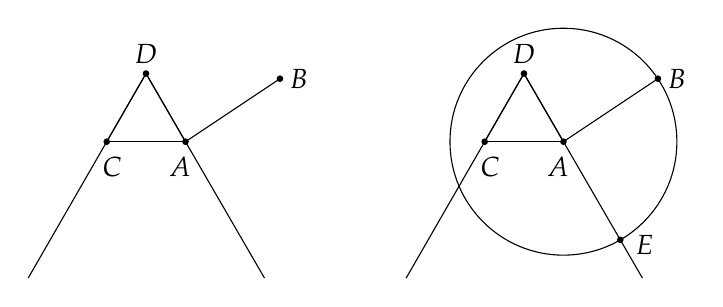
\begin{tikzpicture}[scale=0.4]
\begin{scope}
\coordinate (C) at (0,0);
\coordinate (A) at (2.5,0);
\coordinate (B) at (5.5,2);
\draw (A) node[below,xshift=-2pt,yshift=-2pt] {$A$} -- (B) node[right] {$B$};
\fill (A) circle[radius=3pt];
\fill (B) circle[radius=3pt];
\fill (C) node[below,xshift=2pt,yshift=-2pt] {$C$} circle[radius=3pt];
\draw (A) -- (C);
\path[name path=larc] (C) ++(-70:2.5cm) arc (-70:70:2.5cm);
\path[name path=rarc] (A) ++(-110:2.5cm) arc (-110:-250:2.5cm);
\path [name intersections={of=larc and rarc,by={d,D}}];
\fill (D) node[above] {$D$} circle[radius=3pt];
\draw (A) -- (D);
\draw (C) -- (D);
\draw[name path=ray2] (D) -- ($ (D) ! 3 ! (C) $);
\draw[name path=ray1] (D) -- ($ (D) ! 3 ! (A) $);
\end{scope}
\begin{scope}[xshift=12cm]
\coordinate (C) at (0,0);
\coordinate (A) at (2.5,0);
\coordinate (B) at (5.5,2);
\draw (A) node[below,xshift=-2pt,yshift=-2pt] {$A$} -- (B) node[right] {$B$};
\fill (A) circle[radius=3pt];
\fill (B) circle[radius=3pt];
\fill (C) node[below,xshift=2pt,yshift=-2pt] {$C$} circle[radius=3pt];
\draw (A) -- (C);
\path[name path=larc] (C) ++(-70:2.5cm) arc (-70:70:2.5cm);
\path[name path=rarc] (A) ++(-110:2.5cm) arc (-110:-250:2.5cm);
\path [name intersections={of=larc and rarc,by={d,D}}];
\fill (D) node[above] {$D$} circle[radius=3pt];
\draw (A) -- (D);
\draw (C) -- (D);
\draw[name path=ray2] (D) -- ($ (D) ! 3 ! (C) $);
\draw[name path=ray1] (D) -- ($ (D) ! 3 ! (A) $);
\node[draw,circle through=(B),name path=c1] at (A) {};
\path [name intersections={of=c1 and ray1,by={E,e}}];
\fill (E) node[right,xshift=2pt,yshift=-2pt] {$E$} circle[radius=3pt];
\end{scope}
\end{tikzpicture}
\end{center}

Construct a circle centered at $D$ with radius $DE$. Label the intersection of the circle and the ray $DC$ by $F$:

\vspace*{-2ex}

\begin{center}
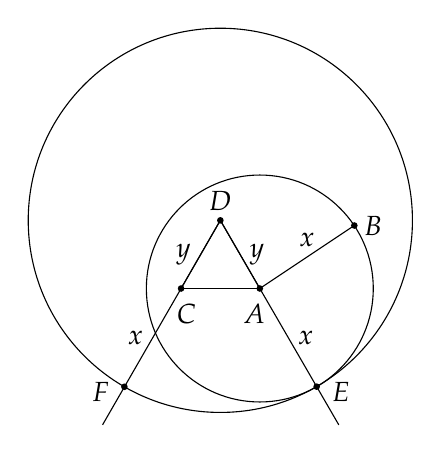
\begin{tikzpicture}[scale=0.4]
\coordinate (C) at (0,0);
\coordinate (A) at (2.5,0);
\coordinate (B) at (5.5,2);
\draw (A) node[below,xshift=-2pt,yshift=-2pt] {$A$} -- node[above] {$x$} (B) node[right] {$B$};
\fill (A) circle[radius=3pt];
\fill (B) circle[radius=3pt];
\fill (C) node[below,xshift=2pt,yshift=-2pt] {$C$} circle[radius=3pt];
\draw (A) -- (C);
\path[name path=larc] (C) ++(-70:2.5cm) arc (-70:70:2.5cm);
\path[name path=rarc] (A) ++(-110:2.5cm) arc (-110:-250:2.5cm);
\path [name intersections={of=larc and rarc,by={d,D}}];
\fill (D) node[above] {$D$} circle[radius=3pt];
\draw (A) -- node[right] {$y$} (D);
\draw (C) -- node[left] {$y$} (D);
\draw[name path=ray2] (D) -- ($ (D) ! 3 ! (C) $);
\draw[name path=ray1] (D) -- ($ (D) ! 3 ! (A) $);
\node[draw,circle through=(B),name path=c1] at (A) {};
\path [name intersections={of=c1 and ray1,by={E,e}}];
\fill (E) node[right,xshift=2pt,yshift=-2pt] {$E$} circle[radius=3pt];
\node[draw,circle through=(E),name path=c2] at (D) {};
\path [name intersections={of=c2 and ray2,by={F,f}}];
\fill (F) node[left,xshift=-2pt,yshift=-2pt] {$F$} circle[radius=3pt];
\path (A) -- node[right] {$x$} (E);
\path (C) -- node[left] {$x$} (F);
\end{tikzpicture}
\end{center}

\vspace*{-1ex}

\textbf{Claim:} The length of the line segment $CF$ is equal to the length of $AB$.

\textbf{Proof:} $DC=DA$ because $\triangle ACD$ is equilateral. $AE=AB$ because they are radii of the same circle centered at $A$. $DF=DE$ because they are radii of the same circle centered at $D$. Therefore, the length of the line segment $CF$ is:

\vspace*{-1ex}

\[
CF=DF-DC=DE-DC=DE-DA=AE=AB\,.
\]


\vspace*{-1ex}

%%%%%%%%%%%%%%%%%%%%%%%%%%%%%%%%%%%%%%%%%%%%%%%%%%%%%%%%%%%%%%%

\section{An incorrect construction for copying a line segment}\label{s.erroneous}

\textbf{Construction(\cite{rusty}):}

Construct a circle centered at $A$ with radius $AB$:

\begin{center}
\begin{tikzpicture}[scale=0.4]
\begin{scope}
\coordinate (C) at (-2,0);
\coordinate (A) at (2.5,0);
\coordinate (B) at (4.5,1.5);
\draw (A) node[below,xshift=-2pt,yshift=-2pt] {$A$} -- (B) node[right] {$B$};
\fill (A) circle[radius=3pt];
\fill (B) circle[radius=3pt];
\fill (C) node[below,xshift=2pt,yshift=-2pt] {$C$} circle[radius=3pt];
\end{scope}
\begin{scope}[xshift=12cm]
\coordinate (C) at (-2,0);
\coordinate (A) at (2.5,0);
\coordinate (B) at (4.5,1.5);
\draw (A) node[below,xshift=-2pt,yshift=-2pt] {$A$} -- (B) node[right] {$B$};
\fill (A) circle[radius=3pt];
\fill (B) circle[radius=3pt];
\fill (C) node[below,xshift=2pt,yshift=-2pt] {$C$} circle[radius=3pt];
\node[draw,circle through=(B),name path=c1] at (A) {};
\end{scope}
\end{tikzpicture}
\end{center}

Construct a circle centered at $A$ with radius $AC$ and a circle centered at $C$ with radius $AC=CA$. Label the intersections of the two circles $E,F$. Label the intersection of the circle centered at $C$ and the circle centered at $A$ with radius $AB$ by $D$:

\begin{center}
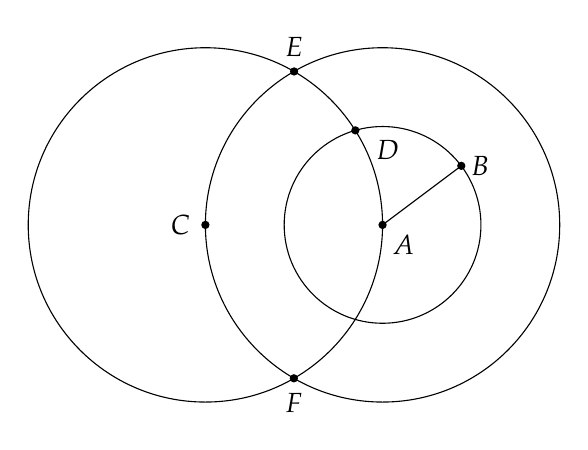
\begin{tikzpicture}[scale=0.5]
\coordinate (C) at (-2,0);
\coordinate (A) at (2.5,0);
\coordinate (B) at (4.5,1.5);
\draw (A) node[below right] {$A$} -- (B) node[right] {$B$};
\fill (A) circle[radius=3pt];
\fill (B) circle[radius=3pt];
\fill (C) node[left,xshift=-2pt] {$C$} circle[radius=3pt];
\node[draw,circle through=(B),name path=c1] at (A) {};
\node[draw,circle through=(C),name path=c2] at (A) {};
\node[draw,circle through=(A),name path=c3] at (C) {};
\path [name intersections={of=c1 and c3,by={D,f}}];
\path [name intersections={of=c2 and c3,by={E,F}}];
\fill (D) node[below right,xshift=4pt] {$D$} circle[radius=3pt];
\fill (E) node[above,yshift=2pt] {$E$} circle[radius=3pt];
\fill (F) node[below,yshift=-2pt] {$F$} circle[radius=3pt];
\end{tikzpicture}
\end{center}

Construct a circle centered at $E$ with radius $ED$. Label the intersection of this circle with the circle centered at $A$ with radius $AC$ by $G$:

\begin{center}
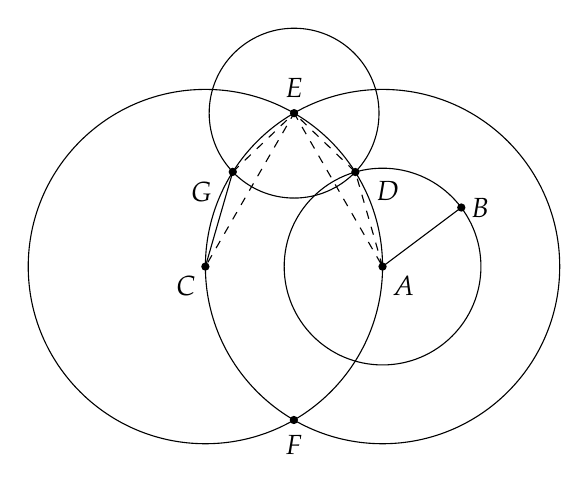
\begin{tikzpicture}[scale=0.5]
\coordinate (C) at (-2,0);
\coordinate (A) at (2.5,0);
\coordinate (B) at (4.5,1.5);
\draw (A) node[below right] {$A$} -- (B) node[right] {$B$};
\fill (A) circle[radius=3pt];
\fill (B) circle[radius=3pt];
\fill (C) node[below left] {$C$} circle[radius=3pt];
\node[draw,circle through=(B),name path=c1] at (A) {};
\node[draw,circle through=(C),name path=c2] at (A) {};
\node[draw,circle through=(A),name path=c3] at (C) {};
\path [name intersections={of=c1 and c3,by={D,f}}];
\path [name intersections={of=c2 and c3,by={E,F}}];
\fill (D) node[below right,xshift=4pt] {$D$} circle[radius=3pt];
\fill (E) node[above,yshift=2pt] {$E$} circle[radius=3pt];
\fill (F) node[below,yshift=-2pt] {$F$} circle[radius=3pt];
\node[draw,circle through=(D),name path=c4] at (E) {};
\path [name intersections={of=c2 and c4,by={g,G}}];
\fill (G) node[below left,xshift=-4pt] {$G$} circle[radius=3pt];
\draw (C) -- (G);
\draw[dashed] (G) -- (E) -- (C);
\draw[dashed] (A) -- (D) -- (E) -- cycle;
\end{tikzpicture}
\end{center}

\textbf{Claim:} The length of the line segment $GC$ is equal to the length of $AB$.

\textbf{Proof:} We shall show that $\triangle ADE\cong\triangle CGE$. If so, $CG=AD=AB$ because $AB,AD$ are radii of the smaller circle centered at $A$. The circle centered at $C$ has the same radius as the circle centered at $A$ that goes through $E$, so we can consider that they are the ``same'' circle.

$EG=ED$ because they are radii of the circle centered at $E$ and $EC=EA$ because they are radii of the ``same'' circle. $\angle GCE=\angle DAE$ because they are central angles that intercept the ``same'' chord and $\angle CGE=\angle ADE$ because they are inscribed angles intercepting the ``same'' chord. Therefore, $\angle GEC=\angle DEA$ and $\triangle GEC\cong \triangle DAE$ by SAS. 

The answer: there isn't any error in the proof! The problem arises from a different source: the equality $AB=GC$ holds only when the length of $AB$ is less that the length of $AC$. In contrast, Euclid's construction and proof are true, independent of the relative lengths of  $AB$ and $AC$, and of the position of the point $C$ relative to the line segment $AB$ (\cite{toussaint}).


%%%%%%%%%%%%%%%%%%%%%%%%%%%%%%%%%%%%%%%%%%%%%%%%%%%%%%%%%%%%%%%

\section{A ``simpler'' construction for copying a line segment}

Given a line segment $AB$ and a point $C$, if we can build a parallelogram with these three points as its vertices, we obtain a line segment with $C$ at one end whose length is equal to the length of $AB$ (left diagram left):
\begin{center}
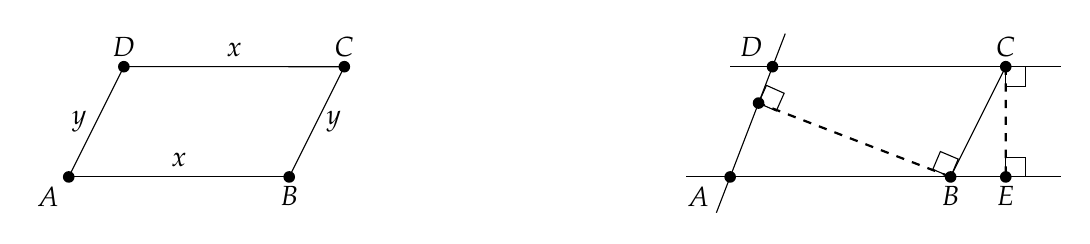
\begin{tikzpicture}[scale=0.7]
\coordinate (A) at (0,0);
\coordinate (B) at (4,0);
\coordinate (C) at (5,2);
\draw (A) -- (B);
\path (A) -- node[above] {$x$} (B);
\fill (A) node[below left] {$A$} circle[radius=3pt];
\fill (B) node[below] {$B$} circle[radius=3pt];
\fill (C) node[above] {$C$} circle[radius=3pt];
\draw (B) -- node[right] {$y$} (C);
\coordinate (D) at ($(C)+(-40mm,0cm)$);
\draw (D) -- node[above] {$x$} (C);
\draw (A) -- node[left] {$y$} (D);
\fill (D) node[above] {$D$} circle[radius=3pt];
\begin{scope}[xshift=12cm]
\coordinate (A) at (0,0);
\coordinate (B) at (4,0);
\coordinate (C) at (5,2);
\draw ($ (B) ! 1.2 ! (A) $) -- ($ (A) ! 1.5 ! (B) $);
\path (A) -- (B);
\fill (A) node[below left,xshift=-4pt] {$A$} circle[radius=3pt];
\fill (B) node[below] {$B$} circle[radius=3pt];
\fill (C) node[above] {$C$} circle[radius=3pt];
\draw (B) -- (C);
\draw[name path=ray1] ($(C)+(-5cm,0cm)$) -- ($(C)+(1cm,0cm)$);
\draw[name path=ray2] ($(A)+(-.25,-.65)$) -- ($(A)+(1,2.6)$);
\path [name intersections={of=ray1 and ray2,by={D}}];
\fill (D) node[above left] {$D$} circle[radius=3pt];
\coordinate (E) at (C |- B);
\draw[thick,dashed] (C) -- (E);
\fill (E) node[below] {$E$} circle[radius=3pt];
\draw[rotate=-90] (C) rectangle +(10pt,10pt);
\draw (E) rectangle +(10pt,10pt);
\coordinate (F) at ($(A)!(B)!(D)$);
\fill (F) circle[radius=3pt];
\draw[thick,dashed] (B) -- (F);
\draw[rotate=-24] (F) rectangle +(10pt,10pt);
\draw[rotate=67] (B) rectangle +(10pt,10pt);
\end{scope}
\end{tikzpicture}
\end{center}
This construction can be found in \cite[pp. 207--208]{roads}.

\textbf{Construction (right diagram):}

Construct the line segment from $B$ to $C$.

Construct an altitude from $C$ to the line containing the line segment $AB$. Label the intersection by $D$.

Construct an altitude to the line segment $CD$ at $C$. This line is parallel to $AB$.

Use a similar method to construct a line parallel to $BC$ through $A$. Label the intersection of the two lines by $D$.

$AD\|BC$, $AB\|DC$ and by definition $ABCD$ is a parallelogram, so $AB=CD$ as required.

\textbf{Construction with a collapsing compass:} We will show that it is possible to construct an altitude through a given point with a collapsing compass. Construct a circle centered at $C$ with a radius that is greater than the distance of $C$ from the line. Label the intersections with the line by $D,E$. Construct circles centered at $D,E$ with radii $DC=EC$:
\begin{center}
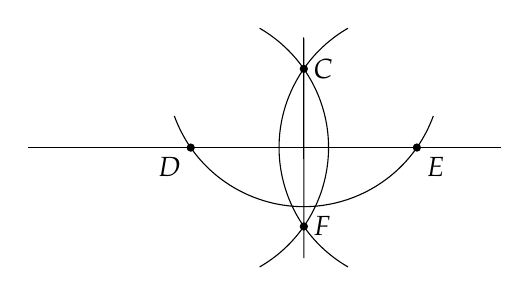
\begin{tikzpicture}[scale=0.5]
\coordinate (A) at (0,0);
\coordinate (B) at (4,0);
\coordinate (C) at (5,2);
\draw[name path=ray] ($ (B) ! 1.5 ! (A) $) -- ($ (A) ! 2.5 ! (B) $);
%\fill (A) node[below] {$A$} circle[radius=3pt];
%\fill (B) node[below] {$B$} circle[radius=3pt];
\fill (C) node[right] {$C$} circle[radius=3pt];
\draw[name path=arc] (C) ++(-160:3.5cm) arc (-160:-20:3.5cm);
\path [name intersections={of=arc and ray,by={D,E}}];
\fill (D) node[below left] {$D$} circle[radius=3pt];
\fill (E) node[below right] {$E$} circle[radius=3pt];
\draw[name path=larc] (D) ++(-60:3.5cm) arc (-60:60:3.5cm);
\draw[name path=rarc] (E) ++(-120:3.5cm) arc (-120:-240:3.5cm);
\path [name intersections={of=larc and rarc,by={b,t}}];
\fill (b) node[right] {$F$} circle[radius=3pt];
\draw ($ (b) ! 1.2 ! (t)$) -- ($ (t) ! 1.2 ! (b)$);
\end{tikzpicture}
\end{center}
The line connecting the intersections of the circles $C,F$ is an altitude through $C$.

The proof the correctness of this construction is much more difficult than Euclid's proof of his construction.

%%%%%%%%%%%%%%%%%%%%%%%%%%%%%%%%%%%%%%%%%%%%%%%%%%%%%%%%%%%%%%%

\section{Don't trust a diagram}

In Section~\ref{s.erroneous}, we saw that a diagram can lead us astray. Here is a proof that \emph{all} triangles are isosceles!
\begin{center}
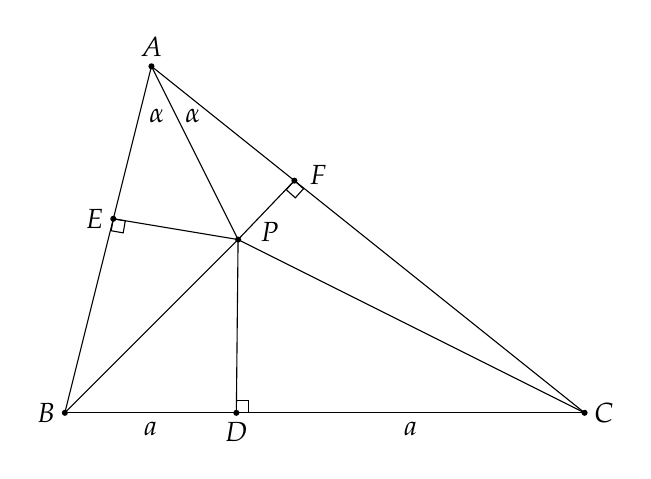
\begin{tikzpicture}[scale=1.1]
\coordinate (P) at (0,0);
\node[xshift=4mm,yshift=1mm] at (P) {$P$};
\coordinate [label=left:$B$] (B)  at (-2,-2);
\coordinate [label=right:$C$] (C)  at (4,-2);
\coordinate [label=above:$A$] (A)  at (-1,2);
\node[below,yshift=-12pt,xshift=2pt] at (A) {$\alpha$};
\node[below,yshift=-12pt,xshift=15pt] at (A) {$\alpha$};
\draw (A) -- (B);
\draw (A) -- (C);
\draw (B) -- (C);
\draw (A) -- (P);
\draw (B) -- (P);
\draw (C) -- (P);
\coordinate[label=left:$E$] (E) at ($ (A) ! .44 ! (B) $);
\draw[rotate=-100] (E) rectangle +(4pt,4pt);
\draw (P) -- (E);
\coordinate (F) at ($ (A) ! .33 ! (C) $);
\node[right,xshift=2pt,yshift=2pt] at (F) {$F$};
\draw[rotate=-132] (F) rectangle +(4pt,4pt);
\draw (P) -- (F);
\coordinate[label=below:$D$] (D) at ($ (B) ! .33 ! (C) $);
\draw (D) rectangle +(4pt,4pt);
\draw (P) -- (D);
\node[left] at ($ (A) ! .5 ! (E) $) {};
\node[left] at ($ (B) ! .5 ! (E) $) {};
\node[below] at ($ (B) ! .5 ! (D) $) {$a$};
\node[below] at ($ (C) ! .5 ! (D) $) {$a$};
\node[right,xshift=2pt] at ($ (A) ! .5 ! (F) $) {};
\node[right,xshift=2pt] at ($ (C) ! .5 ! (F) $) {};
\foreach \n in {A,B,C,D,E,F,P} {
  \fill (\n) circle[radius=1pt];
}
\end{tikzpicture}
\end{center}
Given an arbitrary triangle $\triangle ABC$, let $P$ be the intersection of the angle bisector of $\angle BAC$ and the perpendicular bisector $BC$. Label by $D,E,F$ the intersections of the altitudes from $P$ to the sides $BC, AB,AC$. $\triangle APF\cong \triangle APE$ because they are right triangles with equal angles $\alpha$ and a common side $AP$.

$\triangle DPC\cong \triangle DPB$ SAS because $PD$ is a common side, $\angle PDB=\angle PDC=90$ and $BD=DC=a$ because $PD$ is the perpendicular bisector of $BC$. $\triangle EPB\cong \triangle EPC$ because $EP=PF$ by the first congruence and $PB=PC$ by the second congruence. By combining the equations we get that $\triangle ABC$ is isoceles:
\[
AB= AE+EB=AF+FC =AC\,.
\]
The problem with the proof is that the diagram is incorrect because point $P$ is \emph{outside} the triangle, as can be seen from the following diagram constructed using GeoGebra:
\begin{center}
\includegraphics[width=.5\textwidth]{isoceles}
\end{center}



\tikzsetfigurename{trisect-an-angle}
% !TeX root = construct.tex

\chapter{How to Trisect an Angle (If You Are Willing to Cheat)}\label{c.trisect}

\vspace{-1ex}

It is well known that it is impossible to trisect an arbitrary angle using a compass and a straightedge. The reason is that trisection requires the construction of cube roots, but the compass and straightedge can only construct lengths that are expressions built from the four arithmetic operators and square roots.

Greek mathematicians discovered that if other instruments are allowed, angles can be trisected. Section~\ref{s.neusis} presents a construction of Archimedes using a simple instrument called a neusis. Section~\ref{s.q} shows a more complex construction of Hippias using the quadratrix. As a bonus, Section~\ref{s.square} shows that the quadratrix can square a circle.

References:\\
\url{https://en.wikipedia.org/wiki/Angle_trisection}\\
\url{https://en.wikipedia.org/wiki/Quadratrix_of_Hippias}\\
\url{https://en.wikipedia.org/wiki/Neusis_construction}

%%%%%%%%%%%%%%%%%%%%%%%%%%%%%%%%%%%%%%%%%%%%%%%%%%%%%%%%%%%%%

\vspace{-1ex}

\section{Trisection using the neusis}\label{s.neusis}

In geometry textbooks, constructions are performed using a ``straightedge'' and a compass. The term straightedge is used instead of ``ruler'' because a straightedge has no marks on it. The only operation it can perform is to construct a straight line between two points, while a ruler can measure distances. To trisect an angle all we need is a straightedge with two marks that are a fixed distance apart, called a \emph{neusis}. We define the distance between the marks as $1$:
\begin{center}
\begin{tikzpicture}[scale=3.5]
\draw (-1,1.05) rectangle +(3.2,.1);
\draw[thick] (1.89,1.05) -- +(0,.1);
\draw[thick] (.73,1.05) -- +(0,.1);
\draw[<->] (.73,1.25) -- node[fill=white] {$1$} (1.89,1.25);
\end{tikzpicture}
\end{center}

Let $\alpha$ be an arbitrary angle $\angle ABE$ within a circle with center $B$ and radius $1$. The circle can be constructed by setting the compass to the distance between the marks on the neusis. Extend the radius $EB$ beyond the circle. Place an edge of the neusis on $A$ and move it until it intersects the extension of $EB$ at $D$ and the circle at $C$, using the marks so that the length of the line segment $CD$ is $1$. Draw the line $AD$:

\begin{center}
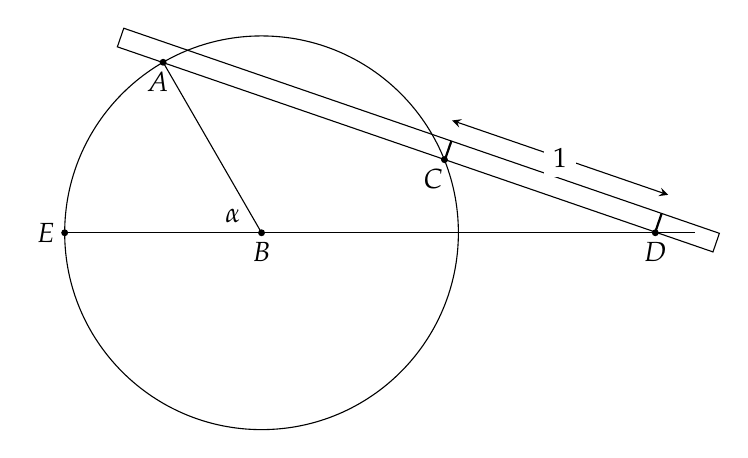
\begin{tikzpicture}[scale=2.5]
\coordinate (origin) at (0,0) node[below] {$B$} ;
\draw[name path=circle] (origin) circle [radius=1];
\draw (origin) node[above left,xshift=-4pt] {$\alpha$} -- (120:1) coordinate (a) node[below,xshift=-2pt] {$A$} ;
\draw (-1,0) -- (2.2,0);
\path[name path=ad] (a) -- (0,0 -| 2,0) coordinate (d) node[below] {$D$} ;
\path[name intersections={of=circle and ad,by={c,a1}}];
\fill (origin) circle [radius=.5pt];
\fill (a) circle [radius=.5pt];
\fill (c) circle [radius=.5pt] node [below,xshift=-4pt] {$C$};
\fill (d) circle [radius=.5pt];
\fill (-1,0) circle [radius=.5pt] node [left] {$E$};
\begin{scope}[rotate=-19,yshift=-11.25pt]
\draw (-1,1.05) rectangle +(3.2,.1);
\draw[thick] (1.89,1.05) -- +(0,.1);
\draw[thick] (.76,1.05) -- +(0,.1);
\draw[<->] (.73,1.25) -- node[fill=white] {$1$} (1.89,1.25);
\end{scope}
\end{tikzpicture}
\end{center}

Draw line $BC$ and label the angles and line segments as shown:

\begin{center}
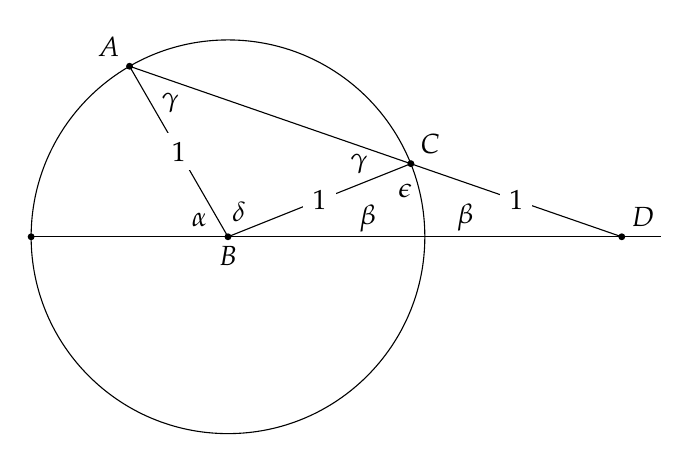
\begin{tikzpicture}[scale=2.5]
\coordinate (origin) at (0,0) node[below] {$B$} ;
\draw[name path=circle] (origin) circle [radius=1];
\draw (origin) node[above left,xshift=-4pt] {$\alpha$} node[above,xshift=4pt,yshift=2pt] {$\delta$} node[above right,xshift=44pt,yshift=-2pt] {$\beta$} -- node[fill=white] {$1$} (120:1) coordinate (a) node[above left] {$A$} ;
\draw (-1,0) -- (2.2,0);
\draw[name path=ad] (a) node[below right,xshift=8pt,yshift=-6pt] {$\gamma$} -- (0,0 -| 2,0) coordinate (d) node[left,xshift=-50pt,yshift=7pt] {$\beta$} node[above right] {$D$} ;
\path[name intersections={of=circle and ad,by={c,a1}}];
\draw (origin) -- node[fill=white] {$1$}(c) node[above right] {$C$} node[left,xshift=-12pt] {$\gamma$} node[below,xshift=-2pt,yshift=-4pt] {$\epsilon$};
\fill (origin) circle [radius=.5pt];
\fill (a) circle [radius=.5pt];
\fill (d) circle [radius=.5pt];
\fill (c) circle [radius=.5pt];
\fill (-1,0) circle [radius=.5pt];
\path (c) -- node[fill=white] {$1$} (d);
%\begin{scope}[rotate=-20]
%\draw (-1,1.05) rectangle +(3.2,.1);
%\draw[thick] (1.89,1.05) -- +(0,.1);
%\draw[thick] (.73,1.05) -- +(0,.1);
%\draw[<->] (.73,1.25) -- node[fill=white] {$1$} (1.89,1.25);
%\end{scope}
\end{tikzpicture}
\end{center}

Both $\triangle ABC$ and $\triangle BCD$ are isoceles: $AB=BC$ since both are radii and $BC=CD$ by construction using the neusis. A computation (using the facts that the angles of a triangle and supplementary angles add up to $\pi$ radians) shows that $\beta$ trisects $\alpha$:
\erh{1pt}
\begin{equationarray*}{rcl}
\epsilon &=& \pi - 2\beta\\
\gamma &=& \pi - \epsilon = 2\beta\\
\delta &=& \pi - 2\gamma = \pi - 4\beta\\
\alpha &=& \pi - \delta - \beta\\
&=& 4\beta -\beta\\
&=& 3\beta\,.
\end{equationarray*}

\vspace{-2ex}

%%%%%%%%%%%%%%%%%%%%%%%%%%%%%%%%%%%%%%%%%%%%%%%%%%%%%%%%%%%%%

\section{Trisection using the quadratrix}\label{s.q}

The following diagram shows a \emph{quadratrix compass}: two (unmarked) straightedges connected by a joint that constrains them to move together. One straightedge moves parallel to the $x$-axis from $DC$ to $AB$, while the second straightedge is allowed to rotate around the origin at $A$ until it lies horizontally along $AB$. The curve traced by the joint of the two straightedges is called the \emph{quadratrix curve} or simply the \emph{quadratrix}.

\begin{center}
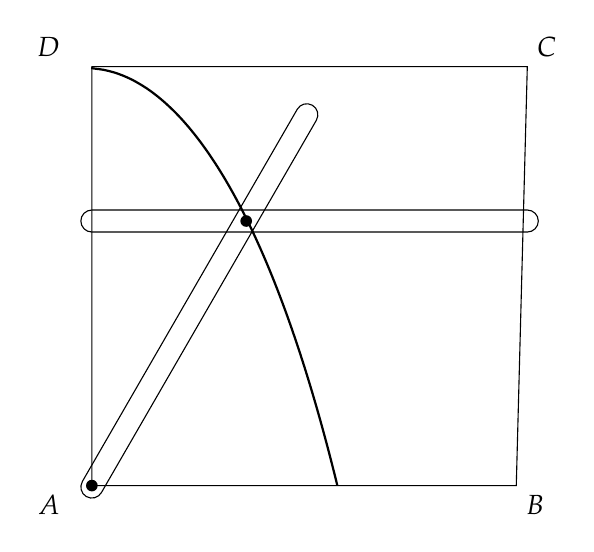
\begin{tikzpicture}[scale=.7,domain=.03:1.555,samples=100]
\draw (.1,.2) node[below left,xshift=-8pt] {$A$} -- (7.8,.2) node[below right] {$B$} -- (8,7.8) node[above right] {$C$} -- (.1,7.8) node[above left,xshift=-8pt] {$D$} -- cycle;
%\draw (.1,7.8) -- (.1,.2) -- (8,.1) -- (8,7.8);
\draw[rounded corners,rotate=60] (0,-.2) rectangle (8.2,.2);
\draw[rounded corners] (-.1,4.8) rectangle (8.2,5.2);
\fill (2.9,5) circle [radius=3pt];
\fill (.1,.2) circle [radius=3pt];
\draw[thick] plot (4.6*.637*\x,{12.2*.637*\x*cot(\x r)});
\end{tikzpicture}
\end{center}

\vspace{-2ex}

As the horizontal straightedge is moved down at a constant velocity, the other straightedge is constrained to move at a constant angular velocity. In fact, that is the definition of the quadratrix curve. As the $y$-coordinate of the horizontal straightedge decreases from $1$ to $0$, the angle of the other straightedge relative to the $x$-axis decreases from $90^\circ$ to $0^\circ$. The following diagram shows how this can be used to trisect an arbitrary angle $\alpha$:

\vspace{-2ex}

\begin{center}
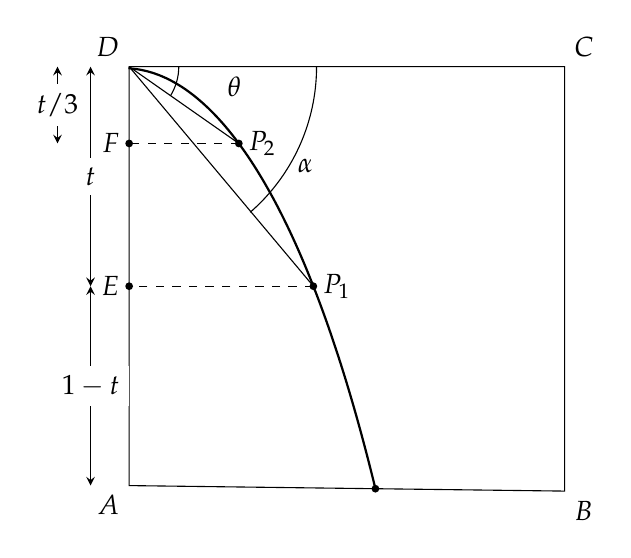
\begin{tikzpicture}[scale=.7,domain=.03:1.562,samples=100]
\draw (.1,7.8) coordinate (start) node[above left] {$D$} node[below right,xshift=32pt] {$\theta$} -- (.1,.2) node[below left] {$A$} -- (8,.1) node[below right] {$B$} -- (8,7.8) node[above right] {$C$} -- cycle;
\draw[name path=curve,thick] plot (4.6*.637*\x,{12.2*.637*\x*cot(\x r)});
% To ensure intersection at node D, path should extend to the upper left of D
\coordinate (twenty-a) at ($(start)+(-35:9)$);
\path[name path=twenty] ($(start)!-.1!(twenty-a)$) -- (twenty-a);
\path[name path=sixty] (start) -- +(-50:9);
\path[name path=xaxis] (.1,.2) -- (8,.1);
\path[name intersections={of=twenty and curve,by={x1,tri}}];
\draw (start) -- (tri);
\fill (tri) circle [radius=2pt] node[right] {$P_2$};
\path[name intersections={of=sixty and curve,by={x2,angle}}];
\fill (angle) circle [radius=2pt] node[right] {$P_1$};
\draw (start) -- (angle);
\path[name intersections={of=xaxis and curve,by=x}];
\fill (x) circle [radius=2pt];
%\path (.1,.2) -- node[below] {$2/\pi$} (x);
\draw[dashed] (tri) -- (tri -| .1,.2) coordinate (t3);
\fill (t3) circle [radius=2pt] node[left] {$F$};
\draw[dashed] (angle) -- (angle -| .1,.2) coordinate (t);
\fill (t) circle [radius=2pt] node[left] {$E$};
\draw[<->] (-1.2,7.8) -- node[fill=white] {$t/3$} (-1.2,7.8 |- t3);
\draw[<->] (-.6,7.8) -- node[fill=white] {$t$} (-.6,7.8 |- t);
\draw[<->] (-.6,7.8 |- t) -- node[fill=white] {$1-t$} (-.6,.2);
\draw (3.5,7.8) arc[start angle=0,delta angle=-49,radius=3.5];
\draw (1,7.8) arc[start angle=0,delta angle=-32,radius=1];
\node at (3.3,6) {$\alpha$}; 
\end{tikzpicture}
\end{center}

\vspace{-2ex}

$P_1$ is the intersection of the line defining the angle $\alpha$ with the quadratrix. This point has $y$-coordinate $1-t$, where $t$ is the distance that the horizontal straightedge has moved from its initial position $DC$. Now trisect the \emph{line segment} $DE$ to obtain point $F$. (It is easy to trisect a line segment using Thales theorem.) Let $P_2$ be the intersection of a line from $F$ parallel to $DC$ and the quadratrix. By the equality of the velocities, we have:

\vspace{-2ex}

\erh{0pt}
\begin{equationarray*}{rcl}
\frac{\theta}{\alpha} &=& \frac{t/3}{t}\\
&&\\
\theta &=& \alpha/3\,.
\end{equationarray*}

\vspace{-3ex}

%%%%%%%%%%%%%%%%%%%%%%%%%%%%%%%%%%%%%%%%%%%%%%%%%%%%%%%%%%%%%

\section{Squaring the circle using the quadratrix}\label{s.square}

\begin{center}
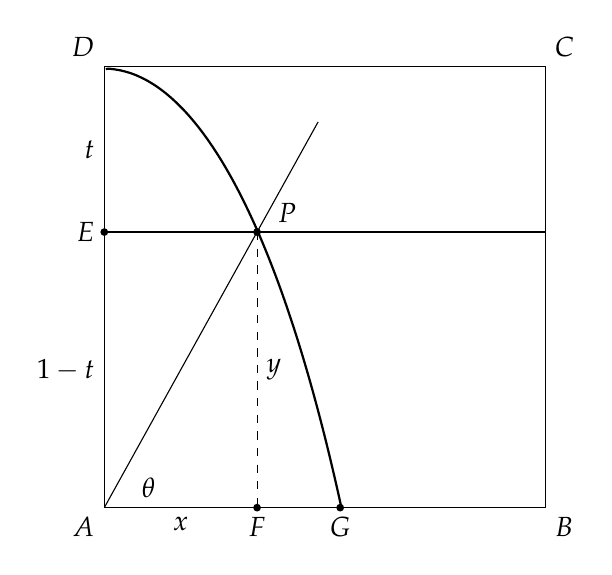
\begin{tikzpicture}[scale=.7,domain=.01:1.57,samples=100]
\draw (0,0) node[below left] {$A$} node [above right,xshift=10pt] {$\theta$} -- (8,0) node[below right] {$B$} -- (8,8) node[above right] {$C$} -- (0,8) node[above left] {$D$} -- cycle;
\draw[name path=horiz] (0,5) -- (8,5);
\draw[name path=slant] (0,0) -- (61:8);
\path[name intersections={of=horiz and slant,by=joint}];
\draw[dashed] (joint) -- node[right] {$y$} (joint |- 0,0) coordinate (f);
\path (0,0) -- node[below] {$x$} (0,0 -| joint) node[below] {$F$};
\path (0,5) node[left] {$E$} -- node[left] {$t$} (0,8);
\path (0,0) -- node[left] {$1-t$} (0,5);
\fill (joint) circle [radius=2pt] node[above right,xshift=4pt] {$P$};
\fill (f) circle [radius=2pt];
\fill (0,5) circle [radius=2pt];
\fill (4.28,0) circle [radius=2pt] node[below] {$G$};
\draw[name path=curve,thick] plot (4.3*.637*\x,{12.5*.637*\x*cot(\x r)});
\end{tikzpicture}
\end{center}

Suppose that the horizontal straightedge has moved $t$ down the $y$-axis to point $E$ and the rotating straightedge forms an angle of $\theta$ with the $x$-axis. $P$ is the intersection of the quadratrix with the horizontal straightedge, and $F$ is the projection of $P$ on the $x$-axis. What are the coordinates of quadratrix at $P$? Clearly, $y=PF=EA=1-t$. On the quadratrix, $\theta$ decreases at the same rate that $t$ increases:
\erh{0pt}
\begin{equationarray*}{rcl}
\frac{1-t}{1} &=& \frac{\theta}{\pi/2}\\
&&\\
\theta &=&\frac{\pi}{2}(1-t)\,.
\end{equationarray*}
Check if this makes sense: when $t=0$, $\theta=\pi/2$ and when $t=1$, $\theta=0$.

The $x$-coordinate of $P$ follows from trigonometry:
\[
\tan \theta = \frac{y}{x}\,.
\]
which gives:
\[
x = \frac{y}{\tan\theta}=y\cot\theta=y\cot \frac{\pi}{2}(1-t)=y\cot \frac{\pi}{2}y\,.
\]
We usually express a function as $y=f(x)$ but it can also be expressed as $x=f(y)$. Let us compute the $x$-coordinate of the point $G$, the intersection of the quadratrix with the $x$-axis. We can't simply plug in $y=0$ because $\cot 0$ is not defined, but we might get lucky by computing the limit of $x$ as $y$ goes to $0$:
\[
x = y\cot \frac{\pi}{2}y = \frac{2}{\pi}\cdot \frac{\pi}{2}y\cot \frac{\pi}{2}y\,.
\]
For convenience, perform a change of variable $z=\disfrac{\pi}{2}y$ and compute the limit:
\[
\lim_{z\rightarrow 0} z\cot z = \lim_{z\rightarrow 0} \frac{z\cos z}{\sin z} = \lim_{z\rightarrow 0} \frac{\cos z}{\disfrac{\sin z}{z}} = \frac{\cos 0}{1} = 1\,,
\]
using the well-known fact that $\displaystyle\lim_{z\rightarrow 0} \frac{\sin z}{z}=1$.
Therefore, as $y\rightarrow 0$:
\[
x \rightarrow \frac{2}{\pi}\cdot \lim_{y\rightarrow 0}\frac{\pi}{2}y\cot \frac{\pi}{2}y = \frac{2}{\pi}\cdot 1 = \frac{2}{\pi}\,.
\]
Using the quadratrix we have constructed a line segment $AG$ whose length is $x=\displaystyle\frac{2}{\pi}$. With an ordinary straightedge and compass it is easy to construct a line segment of length $\sqrt{\disfrac{2}{x}}=\sqrt{\pi}$ and then construct a square whose area is $\pi$.




\tikzsetfigurename{square-a-circle}
% !TeX root = construct.tex

\chapter{How to (Almost) Square a Circle}

\section{Approximations to $\pi$}\label{s.square-intro}

In the nineteenth century it was proved that three constructions are impossible with straightedge and compass: trisecting an angle, duplicating a cube and squaring a circle. Given a line segment defined to have length $1$, the constructible numbers (lengths) are those obtainable from that line segment using the operators $+,-,\times,/,\surd$.

In the constructions in this chapter we need to divide a line segment into three parts; here we show how the division of two lengths can be constructed. Given a line segment of length $1$ and line segments of lengths $a,b$, by similar triangles $1/b=\overline{OD}/a$ so $\overline{OD}=a/b$.

\begin{center}
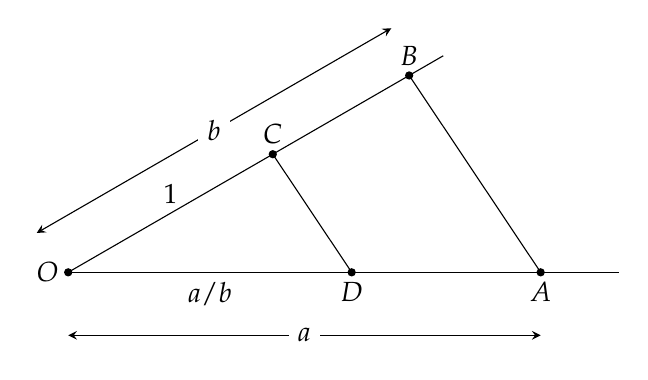
\begin{tikzpicture}
%\clip (-.6,-1) rectangle (4,3);
\draw[name path=horz] (0,0) coordinate (o) -- (7,0);
\fill (o) circle(1.5pt) node[left] {$O$};
\fill (6,0) circle(1.5pt) coordinate (a) node[below] {$A$};
\draw (0,0) -- (30:5.5);
\fill (30:3) circle(1.5pt) coordinate (c) node[above] {$C$};
\fill (30:5) circle(1.5pt) coordinate (b) node[above] {$B$};
\draw (a) -- (b);
\path[name path=par] (c) -- +($(a)-(b)$);
\path[name intersections={of=par and horz,by=d}];
\fill (d) circle(1.5pt) node[below] {$D$};
\draw (c) -- (d);
\draw[<->] (-.4,.5) -- node[fill=white] {$b$} +(30:5.2);
\path (o) -- node[above] {$1$} (c);
\draw[<->] (0,-.8) -- node[fill=white] {$a$} +(6,0);
\path (o) -- node[below] {$a/b$} (d);
\end{tikzpicture}
\end{center}

To square a circle the length $\sqrt{\pi}$ must be constructed, however, $\pi$ is \emph{transcendental}, meaning that it is not the solution of any algebraic equation.

This chapter brings three constructions of approximations to $\pi$. The following table shows the formulas of the lengths that are constructed, their approximate values, the difference between these values and the value of $\pi$, and the error in meters that results if the approximation is used to compute the circumference of the earth given that its radius is $6378$ km.
\[
\renewcommand{\arraystretch}{2.2}
\begin{array}{|l|c|c|c|c|}
\hline
\textrm{Construction} & \textrm{Formula} &\textrm{Value} & \textrm{Difference} & \textrm{Error (m)}\\\hline
\pi & & 3.14159265359 & - & -\\\hline
\textrm{Kochansky} & \sqrt{\disfrac{40}{3}-2\sqrt{3}}&
  3.14153338705 & 5.932 \times 10^{-5} & 756\\\hline
\textrm{Ramanujan}\; 1 & \disfrac{355}{113} &
  3.14159292035 &2.667  \times 10^{-7}&3.4\\\hline
\textrm{Ramanujan}\; 2 &\left(9^2+\disfrac{19^2}{22}\right)^{1/4}&
  3.14159265258 & 1.007 \times 10^{-9}& 0.013\\\hline
\end{array}
\]
Kochansky's construction from $1685$ can be found in \cite{bold}.

Ramanujan's constructions from $1913$ can be found in \cite{ramanujan1,ramanujan2}.

\newpage


%%%%%%%%%%%%%%%%%%%%%%%%%%%%%%%%%%%%%%%%%%%%%%%%%%%%%%%%%%%%%%%%%%%

\section{Kochansky's construction}

Construct three circles:
\begin{enumerate}
\item Construct a unit circle centered at $O$, let $\overline{AB}$ be a diameter and construct a tangent to the circle at $A$.
\item Construct a unit circle centered at $A$. Its intersection with the first circle is $C$.\footnote{For the second and third circles, the diagram only shows the arc that intersects the previous circle.}
\item Construct a unit circle centered at $C$. Its intersection with the second circle is $D$. 
\end{enumerate}
Construct $\overline{OD}$ and denote its intersection with the tangent by $E$.

From $E$ construct $F,G,H$, each at distance $1$ from the previous point; then $\overline{AH}=3-\overline{EA}$.

Construct $\overline{BH}$.

Claim: $\overline{BH}=\sqrt{\disfrac{40}{3}-2\sqrt{3}}\approx \pi$.
\begin{center}
\begin{tikzpicture}[scale=1]
% Scale at 4

% Coordinates of circle
\coordinate (O) at (0,0);
\coordinate (A) at (0,-4);
\coordinate (B) at (0,4);
\fill (O) circle(2pt) node[above right] {$O$};
\fill (A) circle(2pt) node[below right] {$A$};
\fill (B) circle(2pt) node[above right] {$B$};
\draw (A) rectangle +(12pt,12pt);

% Draw circle and diameter
\node [thick,draw,circle through=(A),name path=circle] at (O) {};
\draw [thick] (A) -- (B);

% Draw tangent at A
\draw[thick,name path=tangent] ($(A)+(-4.5,0)$) -- ($(A)+(10.5,0)$);

% Draw arc centered at A which intersects circle at C
\draw[thick,name path=Aarc] (O)
   arc [start angle=90,end angle=220,radius=4];
\path[name intersections={of=circle and Aarc,by=C}];
\fill (C) circle(2pt) node[left,xshift=-4pt] {$C$};

% Draw arc centered at C which intersects the first arc at D
\draw[thick,name path=Carc] ($(C)+(260:4)$)
   arc [start angle=260,end angle=280,radius=4];
\path[name intersections={of=Carc and Aarc,by=D}];
\fill (D) circle(2pt) node[below left] {$D$};

% Draw O--D which intersects the tangent at E
\draw[thick,name path=OD] (O) -- (D);
\path[name intersections={of=tangent and OD,by=E}];
\fill (E) circle(2pt) node[above left] {$E$};

% Find point H at length 3 from E
\coordinate (F) at ($(E)+(4,0)$);
\fill (F) circle(2pt) node[above right,xshift=4pt] {$F$};
\coordinate (G) at ($(F)+(4,0)$);
\fill (G) circle(2pt) node[above] {$G$};
\coordinate (H) at ($(G)+(4,0)$);
\fill (H) circle(2pt) node[above] {$H$};

% Draw BH of length approximately pi
\draw[thick] (B) -- (H);
\end{tikzpicture}
\end{center}

\newpage

To prove the claim extract the following diagram from the first one. Dashed line segments have been added. Since all the circles are unit circles, it is easy to see that the length of each dashed line segment is $1$. It follows that  $\overline{AOCD}$ is a rhombus so its diagonals are perpendicular to and bisect each other at $K$, so $\overline{AK}=\frac{1}{2}$.
\begin{center}
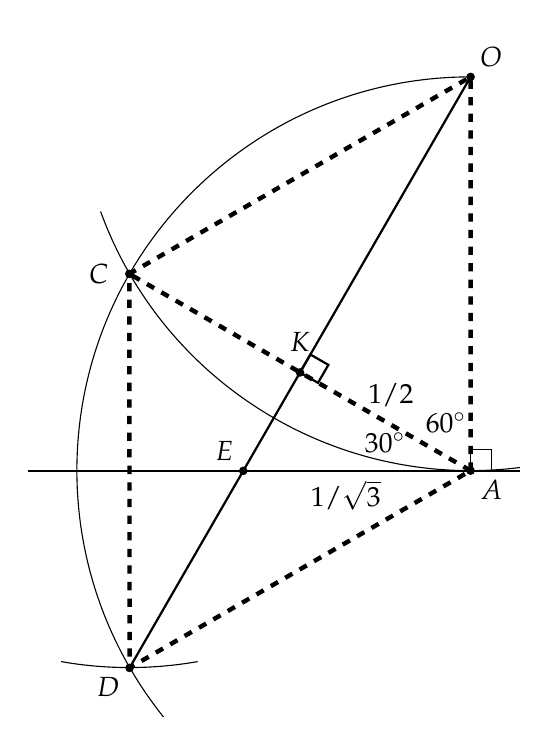
\begin{tikzpicture}[scale=1.25]
% Scale at 4

\clip (-4.5,-6.5) rectangle +(5,7);
% Coordinates of circle
\coordinate (O) at (0,0);
\coordinate (A) at (0,-4);
\coordinate (B) at (0,4);

% Draw circle
\node [circle through=(A),name path=circle] at (O) {};
\draw ($(O)+(200:4)$) arc [start angle=200,end angle=280,radius=4];

% Draw tangent at A
\draw[thick,name path=tangent] ($(A)+(-4.5,0)$) -- ($(A)+(10.5,0)$);
\draw (A) rectangle +(6pt,6pt);

% Draw arc centered at O which intersects circle at C
\draw[thin,name path=Aarc] (O)
   arc [start angle=90,end angle=220,radius=4];
\path[name intersections={of=circle and Aarc,by=C}];

% Draw arc centered at C which intersects the first arc at D
\draw[thin,name path=Carc] ($(C)+(260:4)$)
   arc [start angle=260,end angle=280,radius=4];
\path[name intersections={of=Carc and Aarc,by=D}];

% Draw O--D which intersects the tangent at E
\draw[thick,name path=OD] (O) -- (D);
\path[name intersections={of=tangent and OD,by=E}];

% Find point H at length 3 from E
\coordinate (F) at ($(E)+(4,0)$);
\coordinate (G) at ($(F)+(4,0)$);
\coordinate (H) at ($(G)+(4,0)$);

% Draw BH of length approximately pi
\draw[thick] (B) -- (H);

\draw[ultra thick,dashed] (A) -- (O) -- (C) -- (D) -- cycle;
\draw[ultra thick,dashed,name path=AC] (A) -- (C);

\node[above left,yshift=10pt,xshift=2pt] at (A) {$60^\circ$};
\node[left,yshift=10pt,xshift=-20pt] at (A) {$30^\circ$};

\path[name intersections={of=AC and OD,by=K}];
\draw[thick,rotate=-30] (K) rectangle +(6pt,6pt);

\path (A) -- node[above,xshift=2pt,yshift=2pt] {$1/2$} (K);
\path (A) -- node[below,xshift=-4pt] {$1/\sqrt{3}$} (E);

\fill (O) circle(1.25pt) node[above right] {$O$};
\fill (A) circle(1.25pt) node[below right] {$A$};
\fill (B) circle(1.25pt) node[above right] {$B$};
\fill (C) circle(1.25pt) node[left,xshift=-4pt] {$C$};
\fill (D) circle(1.25pt) node[below left] {$D$};
\fill (E) circle(1.25pt) node[above left] {$E$};
\fill (F) circle(1.25pt) node[above right,xshift=4pt] {$F$};
\fill (G) circle(1.25pt) node[above] {$G$};
\fill (H) circle(1.25pt) node[above] {$H$};
\fill (K) circle(1.25pt) node[above,yshift=4pt] {$K$};
\end{tikzpicture}
\end{center}
The diagonal $\overline{AC}$ forms two equilateral triangles $\triangle OAC, \triangle DAC$ so $\angle OAC=60^\circ$. Since tangent forms a right angle with the radius $\overline{OA}$, $\angle KAE=30^\circ$. Now:
\begin{displaymath}
\renewcommand{\arraystretch}{1.5}
\begin{array}{lcl}
\disfrac{1/2}{\overline{EA}}&=&
\cos 30^\circ=\disfrac{\sqrt{3}}{2}\\
\overline{EA}&=&\disfrac{1}{\sqrt{3}}\\
\overline{AH}&=&3-\overline{EA}=\left(3-\disfrac{1}{\sqrt{3}}\right)
=\disfrac{3\sqrt{3}-1}{\sqrt{3}}\\
\end{array}
\end{displaymath}

Returning to the first diagram, we see that $\triangle ABH$ is a right triangle:
\begin{displaymath}
\renewcommand{\arraystretch}{2}
\begin{array}{lcl}
\overline{BH}^2&=&\overline{OB}^2+\overline{AH}^2\\
&=&4+\disfrac{9\cdot 3 -6\sqrt{3}+1}{3}=\disfrac{40}{3}-2\sqrt{3}\\
\overline{BH}&=&\sqrt{\disfrac{40}{3}-2\sqrt{3}}\approx 3.141533387=\approx \pi\,.
\end{array}
\end{displaymath}

\newpage


%%%%%%%%%%%%%%%%%%%%%%%%%%%%%%%%%%%%%%%%%%%%%%%%%%%%%%%%%%%%%%%%%%%



\section{Ramanujan's first construction}


\subsection{The construction}

Construct a unit circle centered at $O$ and let $\overline{PR}$ be a diameter. 

$H$ bisects $\overline{PO}$ and $T$ trisects $\overline{RO}$. 

Construct a perpendicular at $T$ that intersects the circle at $Q$.

Construct a chord $\overline{RS}=\overline{QT}$.

Construct $\overline{PS}$.

Construct a line parallel to $RS$ from $T$ that intersects $\overline{PS}$ at $N$.

Construct a line parallel to $\overline{RS}$ from $O$ that intersects $\overline{PS}$ at $M$.

Construct the chord $\overline{PK}=\overline{PM}$.

Construct the tangent at $P$ of length $\overline{PL}=\overline{MN}$.

Connect the points $K,L,R$.

Find point $C$ such that $\overline{RC}$ is equal to $\overline{RH}$.

Construct $\overline{CD}$ parallel to $\overline{KL}$ that intersects $\overline{LR}$ at $D$. 

Claim: $\overline{RD}^2=\disfrac{355}{113}\approx pi$.


\begin{center}
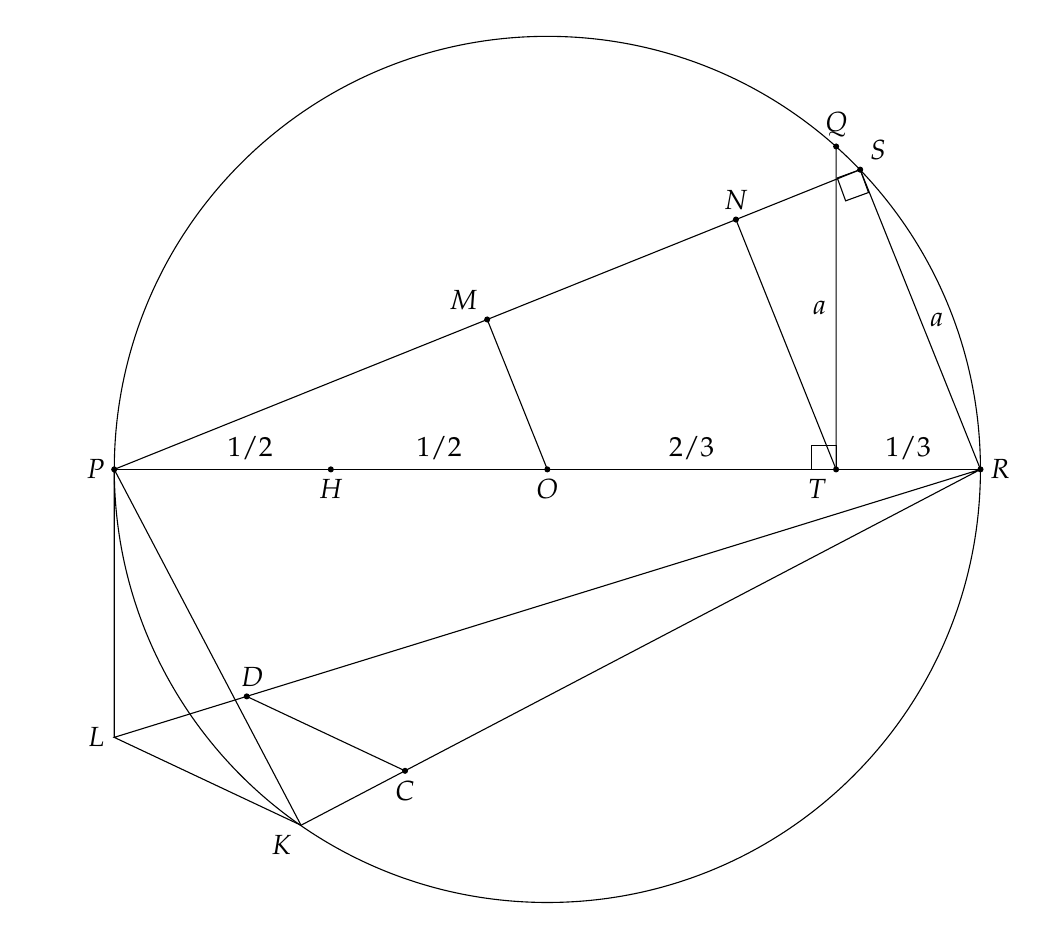
\begin{tikzpicture}[scale=1.1,align=left]
\clip (-6,-5.1) rectangle +(11.5,10.2);
% Draw circle and horizontal diameter
\draw[name path=circle] (0,0)  coordinate (o) node[below] {$O$} circle[radius=5cm];
\draw (-5,0) coordinate (p) node[left] {$P$} -- (5,0) coordinate (r) node[right] {$R$};
\fill (o) circle (1pt);
\fill (p) circle (1pt);
\fill (r) circle (1pt);
\fill (-2.5,0) coordinate (h) node[below] {$H$} circle (1pt);
\fill (10/3,0) coordinate (t) node[below left] {$T$} circle (1pt);
\path (p) -- node[above,xshift=10pt] {$1/2$} (h) -- node[above] {$1/2$} (o) -- node[above] {$2/3$} (t) -- node[above] {$1/3$} (r);

% Draw perpendicular TQ
\path[name path=tq] (t) -- +(0,5);
\path[name intersections={of=tq and circle,by=q}];
\draw (t) -- node[left] {$a$} (q) node[above] {$Q$};
\fill (q) circle (1pt);

% Draw chord RS and line PS
\path[name path=tq] (t) -- +(0,5);
\path[name intersections={of=tq and circle,by=q}];
\path[name path=rcirc] (r) let \p1 = ($ (t) - (q) $) in circle ({veclen(\x1,\y1)});
\path[name intersections={of=rcirc and circle,by=s}];
\draw (r) -- node[right] {$a$} (s);
\fill (s) node[above right] {$S$} circle (1pt);
\draw[name path=ps] (p) -- (s);

% Draw TN
\path[name path=tn] (t) -- +($(s)-(r)$);
\path[name intersections={of=ps and tn,by=n}];
\draw (t) -- (n);
\fill (n) node[above] {$N$} circle (1pt);

% Draw OM
\path[name path=om] (o) -- +($(s)-(r)$);
\path[name intersections={of=ps and om,by=m}];
\draw (o) -- (m);
\fill (m) node[above left] {$M$} circle (1pt);
\path (p) -- (m);
\path (m) -- (n);

% Draw chord PK
\draw (p) -- +(-62.3:4.64) coordinate (k) node[below left] {$K$};

% Draw tangent PL
\draw let \p1 = ($ (m) - (n) $), \n1 = {veclen(\x1,\y1)} in (p) -- (-5,-\n1) coordinate (l) node[left] {$L$};

% Connect L and K to R
\draw (r) -- (l) -- (k) -- cycle;

% Find point C on RK
\coordinate (c) at ($(r)!7.5cm!(k)$);
\path (r) -- (c);
\fill (c) node[below] {$C$} circle (1pt);

% Draw CD
\path[name path=cd] (c) -- +($(l)-(k)$);
\path[name path=lr] (l) -- (r);
\path[name intersections={of=cd and lr,by=d}];
\draw (c) -- (d);
\fill (d) node[above,xshift=2pt] {$D$} circle (1pt);
\path (r) -- (d);

\draw[rotate=90] (t) rectangle +(8pt,8pt);
\draw[rotate=-160] (s) rectangle +(8pt,8pt);
\end{tikzpicture}
\end{center}

\newpage

\subsection{The computation}

By Pythagoras' theorem on $\triangle QOT$:
\[
\overline{QT} = \sqrt{1^2-\left(\frac{2}{3}\right)^2}=\frac{\sqrt{5}}{3}\,.
\]
$\triangle PSR$ is a right triangle because it subtends a diameter. By Pythagoras theorem:
\[
\overline{PS} = \sqrt{2^2-\left(\frac{\sqrt{5}}{3}\right)^2}=\sqrt{4-\frac{5}{9}}=\frac{\sqrt{31}}{3}\,.
\]
$\triangle MPO\sim \triangle SPR$ so:
\begin{form}{2.2}
\disfrac{\overline{PM}}{\overline{PO}}&=&\disfrac{\overline{PS}}{\overline{PR}}\\
\disfrac{\overline{PM}}{1}&=&\disfrac{\sqrt{31}/3}{2}\\
\overline{PM}&=&\disfrac{\sqrt{31}}{6}\,.
\end{form}
$\triangle NPT\sim \triangle SPR$ so:

\begin{form}{2.2}
\disfrac{\overline{PN}}{\overline{PT}}&=&\disfrac{\overline{PS}}{\overline{PR}}\\
\disfrac{\overline{PN}}{5/3}&=&\disfrac{\sqrt{31}/3}{2}\\
\overline{PN}&=&\disfrac{5\sqrt{31}}{18}\\
\overline{MN}&=&\overline{PN}-\overline{PM}\\
&=&\sqrt{31}\left(\disfrac{5}{18}-\disfrac{1}{6}\right) = \disfrac{\sqrt{31}}{9}\,.
\end{form}

$\triangle PKR$ is a right triangle because it subtends a diameter. By Pythagoras's theorem:
\[
\overline{RK}=\sqrt{2^2-\left(\frac{\sqrt{31}}{6}\right)^2} = \frac{\sqrt{113}}{6}\,.
\]

$\triangle PLR$ is a right triangle because it $\overline{PL}$ is a tangent. By Pythagoras's theorem:
\[
\overline{RL}=\sqrt{2^2+\left(\frac{\sqrt{31}}{9}\right)^2} = \frac{\sqrt{355}}{9}\,.
\]

\newpage

$\overline{RC}=\overline{RH}=\displaystyle\frac{1}{3}+\frac{2}{3}+\frac{1}{2}=\frac{3}{2}$. Since $\overline{CD}$ is parallel to $\overline{LK}$, by similar triangles:
\begin{form}{2.2}
\disfrac{\overline{RD}}{\overline{RC}}&=&\disfrac{\overline{RL}}{\overline{RK}}\\
\disfrac{\overline{RD}}{3/2}&=&\disfrac{\sqrt{355}/9}{\sqrt{113}/6}\\
\overline{RD}&=&\sqrt{\disfrac{355}{113}}\,.
\end{form}

Here is the construction with line segments labeled with their lengths:

\begin{center}
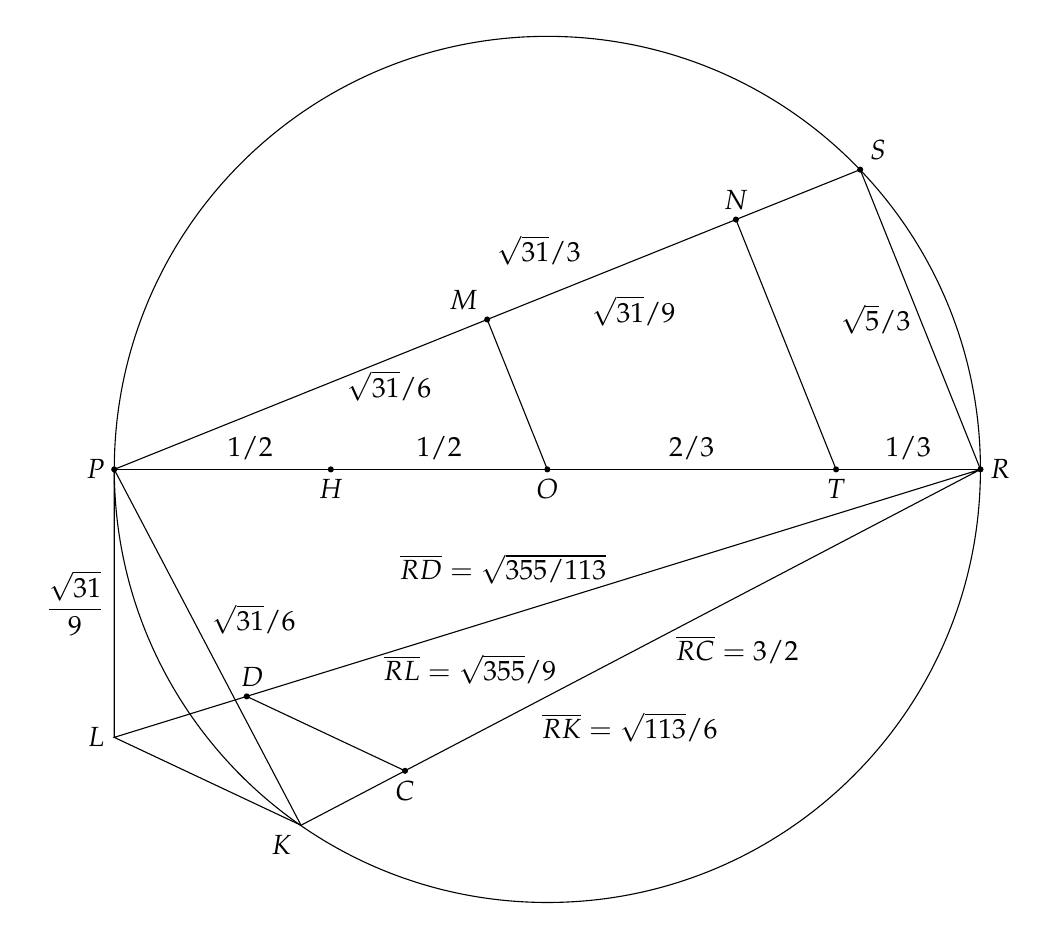
\begin{tikzpicture}[scale=1.1,align=left]
\clip (-6,-5.1) rectangle +(11.5,10.2);
% Draw circle and horizontal diameter
\draw[name path=circle] (0,0)  coordinate (o) node[below] {$O$} circle[radius=5cm];
\draw (-5,0) coordinate (p) node[left] {$P$} -- (5,0) coordinate (r) node[right] {$R$};
\fill (o) circle (1pt);
\fill (p) circle (1pt);
\fill (r) circle (1pt);
\fill (-2.5,0) coordinate (h) node[below] {$H$} circle (1pt);
\fill (10/3,0) coordinate (t) node[below] {$T$} circle (1pt);
\path (p) -- node[above,xshift=10pt] {$1/2$} (h) -- node[above] {$1/2$} (o) -- node[above] {$2/3$} (t) -- node[above] {$1/3$} (r);
% Draw chord RS and line PS
\path[name path=tq] (t) -- +(0,5);
\path[name intersections={of=tq and circle,by=q}];
\path[name path=rcirc] (r) let \p1 = ($ (t) - (q) $) in circle ({veclen(\x1,\y1)});
\path[name intersections={of=rcirc and circle,by=s}];
\draw (r) -- node[left] {$\sqrt{5}/3$} (s);
\fill (s) node[above right] {$S$} circle (1pt);
\draw[name path=ps] (p) -- node[above right,yshift=16pt] {$\sqrt{31}/3$} (s);
% Draw TN
\path[name path=tn] (t) -- +($(s)-(r)$);
\path[name intersections={of=ps and tn,by=n}];
\draw (t) -- (n);
\fill (n) node[above] {$N$} circle (1pt);
% Draw OM
\path[name path=om] (o) -- +($(s)-(r)$);
\path[name intersections={of=ps and om,by=m}];
\draw (o) -- (m);
\fill (m) node[above left] {$M$} circle (1pt);
\path (p) -- node[below,xshift=32pt,yshift=12pt] {$\sqrt{31}/6$} (m);
\path (m) -- node[below,xshift=8pt,yshift=-6pt] {$\sqrt{31}/9$} (n);
% Draw chord PK
\draw (p) -- node[right,xshift=-2pt,yshift=10pt] {$\sqrt{31}/6$} +(-62.3:4.64) coordinate (k) node[below left] {$K$};
% Draw tangent PL
\draw let \p1 = ($ (m) - (n) $), \n1 = {veclen(\x1,\y1)} in (p) -- node[left] {$\disfrac{\sqrt{31}}{9}$} (-5,-\n1) coordinate (l) node[left] {$L$};
% Connect L and K to R
\draw (r) -- (l) -- (k) -- cycle;
% Find point C on RK
\coordinate (c) at ($(r)!7.5cm!(k)$);
%\path (r) -- node[below,yshift=-16pt] {$RC=3/2$\\$RK=\sqrt{113}/6$} (c);
\path (r) -- node[below,xshift=16pt,yshift=-2pt] {$\overline{RC}=3/2$} (c);
\path (r) -- node[below,xshift=-4pt,yshift=-20pt] {$\overline{RK}=\sqrt{113}/6$} (k);
\fill (c) node[below] {$C$} circle (1pt);
% Draw CD
\path[name path=cd] (c) -- +($(l)-(k)$);
\path[name path=lr] (l) -- (r);
\path[name intersections={of=cd and lr,by=d}];
\draw (c) -- (d);
\fill (d) node[above,xshift=2pt] {$D$} circle (1pt);
%\path (r) -- node[above,xshift=-40pt,yshift=-8pt] {$RD=\sqrt{355/113}$\\$RL=\sqrt{355}/9$} (d);
\path (r) -- node[above,xshift=-40pt,yshift=-4pt] {$\overline{RD}=\sqrt{355/113}$} (d);
\path (r) -- node[below,xshift=-28pt,yshift=-15pt] {$\overline{RL}=\sqrt{355}/9$} (l);
\end{tikzpicture}
\end{center}

\bigskip

The value $\disfrac{355}{113}$ could be constructed by constructing two line segments of length $355$ and $113$ and then using the division construction shown in Section~\ref{s.square-intro}, but that is rather tedious!

\newpage

%%%%%%%%%%%%%%%%%%%%%%%%%%%%%%%%%%%%%%%%%%%%%%%%%%%%%%%%%%%%

\section{Ramanujan's second approximation}

\subsection{The construction}

Construct a unit circle centered at $O$ with diameter $\overline{AB}$, and let $C$ be the intersection of the perpendicular at $O$ with the circle.

Trisect $\overline{AO}$ so that $\overline{AT}=1/3$ and $\overline{TO}=2/3$.

Construct $\overline{BC}$ and find points $M,N$ such that $\overline{CM}=\overline{MN}=\overline{AT}=1/3$.

Construct $\overline{AM}$ and $\overline{AN}$ and let $P$ be the point on $\overline{AN}$ such that $\overline{AP}=\overline{AM}$.

From $P$ construct a line parallel to $\overline{MN}$ that intersects $\overline{AM}$ at $Q$.

Construct $\overline{OQ}$ and then from $T$ construct a line parallel to $\overline{OQ}$ that intersects $\overline{AM}$ at $R$.

Construct a line segment $\overline{AS}$ tangent to $A$ of length $\overline{AR}$.

Construct $\overline{SO}$.

Claim: $3\sqrt{\overline{SO}}=\left(9^2+\disfrac{19^2}{22}\right)^{\frac{1}{4}}\approx \pi$.

\begin{center}
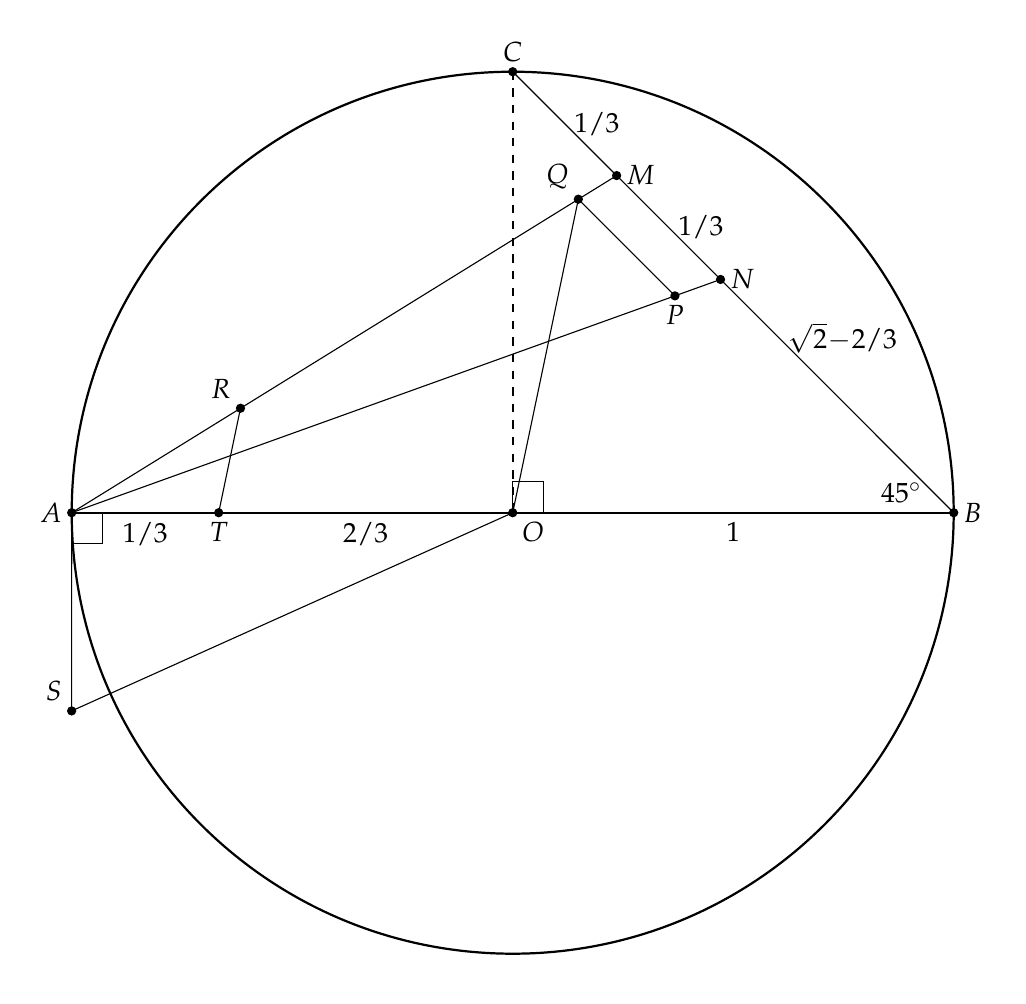
\begin{tikzpicture}[scale=1.4]
\clip (-4.4,-4.2) rectangle +(8.8,8.6);
% Scale at 4

% Coordinates of circle
\coordinate (O) at (0,0);
\coordinate (A) at (-4,0);
\coordinate (B) at (4,0);
\coordinate (C) at (0,4);

% Draw circle and diameter
\node [thick,draw,circle through=(A),name path=circle] at (O) {};
\draw [thick] (A) -- (B);
\draw [thick,dashed] (C) -- (O);
\draw (O) rectangle +(8pt,8pt);
\draw[rotate=-90] (A) rectangle +(8pt,8pt);

\coordinate (T) at (-2.667,0);
\path (A) -- node[below] {$1/3$} (T);
\path (T) -- node[below] {$2/3$} (O);
\path (O) -- node[below] {$1$} (B);

\draw (C) -- node[right] {$1/3$} +(-45:1.333) coordinate (M);
\draw (M) -- node[right] {$1/3$} +(-45:1.333) coordinate (N);
\draw (N) -- node[near start,right] {$\sqrt{2}\!-\!2/3$}(B);

\draw[name path=AM] (A) -- (M);
\draw[name path=AN] (A) -- (N);

\node [circle through=(M),name path=AMcircle] at (A) {};

\path[name intersections={of=AMcircle and AN,by=P}];

\path[name path=PQ] (P) -- +(135:2);
\path[name intersections={of=PQ and AM,by=Q}];
\draw (P) -- (Q) -- (O);

\path[name path=QT] (T) -- ($(Q)+(-2.667,0)$) -- (Q);
\path[name intersections={of=QT and AM,by=R}];
\draw (T) -- (R);

\node [circle through=(R),name path=ARcircle] at (A) {};
\path[name path=AS] (A) -- ($(A)+(0,-2.5)$);
\path[name intersections={of=ARcircle and AS,by=S}];
\draw (A) -- (S);

\draw (S) -- (O);

\fill (O) circle(1.2pt) node[below right] {$O$};
\fill (A) circle(1.2pt) node[left] {$A$};
\fill (B) circle(1.2pt) node[right] {$B$} node[above left,xshift=-8pt] {$45^\circ$};
\fill (C) circle(1.2pt) node[above] {$C$};
\fill (T) circle(1.2pt) node[below] {$T$};
\fill (M) circle(1.2pt) node[right] {$M$};
\fill (N) circle(1.2pt) node[right] {$N$};
\fill (P) circle(1.2pt) node[below] {$P$};
\fill (Q) circle(1.2pt) node[above left] {$Q$};
\fill (R) circle(1.2pt) node[above left] {$R$};
\fill (S) circle(1.2pt) node[above left] {$S$};

\end{tikzpicture}
\end{center}

\newpage

\subsection{Proof}

$\triangle COB$ is a right triangle, $\overline{OB}=\overline{OC}=1$, 	so by Pythagoras' theorem $\overline{CB}=\sqrt{2}$ and $\overline{NB}=\sqrt{2}-2/3$. The triangle is isoceles so $\angle NBA =\angle MBA=45^\circ$.

We use the law of cosines on $\triangle NBA$ to compute $\overline{AN}$:
\begin{form}{2}
\overline{AN}^2&=&\overline{BA}^2 + \overline{BN}^2-2\cdot\overline{BA}\cdot\overline{BN}\cdot\cos \angle NBA\\
&=&2^2+\left(\sqrt{2}-\disfrac{2}{3}\right)^2-2\cdot 2 \cdot \left(\sqrt{2}-\disfrac{2}{3}\right)\cdot \disfrac{\sqrt{2}}{2}\\
&=&\left(4+2+\disfrac{4}{9}-4\right) + \sqrt{2}\cdot \left(-\disfrac{4}{3}+\disfrac{4}{3}\right)=\disfrac{22}{9}\\
\overline{AN}&=&\sqrt{\disfrac{22}{9}}\,.
\end{form}

Similarly, we use the law of cosines on $\triangle MBA$ to compute $\overline{AM}$:
\begin{form}{2}
\overline{AM}^2&=&\overline{BA}^2 + \overline{BM}^2-2\cdot\overline{BA}\cdot\overline{BM}\cdot\cos \angle MBA\\
&=&2^2+\left(\sqrt{2}-\disfrac{1}{3}\right)^2-2\cdot 2 \cdot \left(\sqrt{2}-\disfrac{1}{3}\right)\cdot \disfrac{\sqrt{2}}{2}\\
&=&\left(4+2+\disfrac{1}{9}-4\right) + \sqrt{2}\cdot \left(-\disfrac{2}{3}+\disfrac{2}{3}\right)=\disfrac{19}{9}\\
\overline{AM}&=&\sqrt{\disfrac{19}{9}}\,.
\end{form}

By construction $\overline{QP}\parallel \overline{MN}$ so
$\triangle MAN\sim \triangle QAP$, and by construction $\overline{AP}=\overline{AM}$ giving:
\begin{form}{2.4}
\disfrac{\overline{AQ}}{\overline{AM}}&=&\disfrac{\overline{AP}}{\overline{AN}}=\disfrac{\overline{AM}}{\overline{AN}}\\
\overline{AQ}&=&\disfrac{\overline{AM}^2}{\overline{AN}}=\disfrac{19/9}{\sqrt{22/9}}=\disfrac{19}{3\sqrt{22}}\,.
\end{form}

By construction $\overline{TR}\parallel \overline{OQ}$ so
$\triangle RAT\sim \triangle QAO$ giving:
\begin{form}{2.4}
\disfrac{\overline{AR}}{\overline{AQ}}&=&\disfrac{\overline{AT}}{\overline{AO}}\\
\overline{AR}&=&\overline{AQ}\cdot\disfrac{\overline{AT}}{\overline{AO}}=\disfrac{19}{3\sqrt{22}}\cdot\disfrac{1/3}{1}=\disfrac{19}{9\sqrt{22}}\,.
\end{form}

\newpage

By construction $\overline{AS}=\overline{AR}$ and $\triangle OAS$ is a right triangle. By Pythagoras' theorem:
\begin{form}{3}
\overline{SO}&=&\sqrt{1^2+\left(\disfrac{19}{9\sqrt{22}}\right)^2}\\
3\sqrt{\overline{SO}}&=&3\left(1+\disfrac{19^2}{9^2\cdot 22}\right)^\frac{1}{4}\\
&=&\left(3^4+\disfrac{3^4\cdot 19^2}{9^2\cdot 22}\right)^\frac{1}{4}\\
&=&\left(9^2+\disfrac{19^2}{22}\right)^\frac{1}{4}\approx 3.14159265262\approx \pi\,.
\end{form}

Here is the construction with line segments labeled with their lengths:


\begin{center}
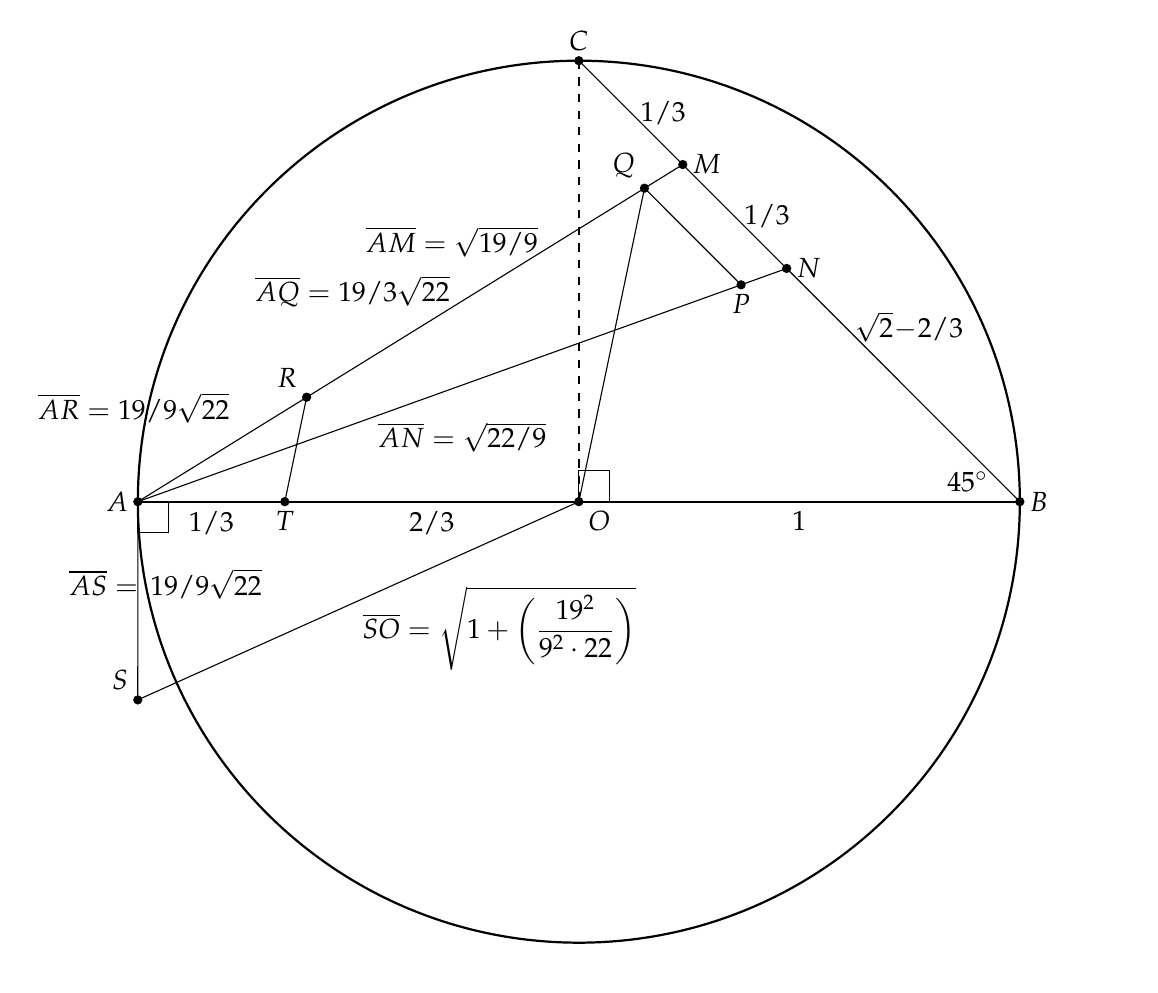
\begin{tikzpicture}[scale=1.4]
\clip (-5,-4.2) rectangle +(10,8.5);
% Scale at 4

% Coordinates of circle
\coordinate (O) at (0,0);
\coordinate (A) at (-4,0);
\coordinate (B) at (4,0);
\coordinate (C) at (0,4);

% Draw circle and diameter
\node [thick,draw,circle through=(A),name path=circle] at (O) {};
\draw [thick] (A) -- (B);
\draw [thick,dashed] (C) -- (O);
\draw (O) rectangle +(8pt,8pt);
\draw[rotate=-90] (A) rectangle +(8pt,8pt);

\coordinate (T) at (-2.667,0);
\path (A) -- node[below] {$1/3$} (T);
\path (T) -- node[below] {$2/3$} (O);
\path (O) -- node[below] {$1$} (B);

\draw (C) -- node[right] {$1/3$} +(-45:1.333) coordinate (M);
\draw (M) -- node[right] {$1/3$} +(-45:1.333) coordinate (N);
\draw (N) -- node[near start,right] {$\sqrt{2}\!-\!2/3$}(B);

\draw[name path=AM] (A) -- node[above,xshift=15pt,yshift=24pt] {$\overline{AM}=\sqrt{19/9}$} (M);
\draw[name path=AN] (A) -- node[below,yshift=-10pt] {$\overline{AN}=\sqrt{22/9}$} (N);

\node [circle through=(M),name path=AMcircle] at (A) {};

\path[name intersections={of=AMcircle and AN,by=P}];

\path[name path=PQ] (P) -- +(135:2);
\path[name intersections={of=PQ and AM,by=Q}];
\draw (P) -- (Q) -- (O);
\path (A) -- node[above,xshift=-14pt,yshift=10pt] {$\overline{AQ}=19/3\sqrt{22}$} (Q);

\path[name path=QT] (T) -- ($(Q)+(-2.667,0)$) -- (Q);
\path[name intersections={of=QT and AM,by=R}];
\draw (T) -- (R);
\path (A) -- node[above,xshift=-32pt,yshift=6pt] {$\overline{AR}=19/9\sqrt{22}$} (R);

\node [circle through=(R),name path=ARcircle] at (A) {};
\path[name path=AS] (A) -- ($(A)+(0,-2.5)$);
\path[name intersections={of=ARcircle and AS,by=S}];
\draw (A) -- node[xshift=10pt,yshift=6pt] {$\overline{AS}=\,19/9\sqrt{22}$} (S);

\draw (S) -- node[right,xshift=-2pt,yshift=-10pt] {$\overline{SO}=\sqrt{1+
  \left(\disfrac{19^2}{9^2\cdot 22}\right)}$} (O);

\fill (O) circle(1.2pt) node[below right] {$O$};
\fill (A) circle(1.2pt) node[left] {$A$};
\fill (B) circle(1.2pt) node[right] {$B$} node[above left,xshift=-8pt] {$45^\circ$};
\fill (C) circle(1.2pt) node[above] {$C$};
\fill (T) circle(1.2pt) node[below] {$T$};
\fill (M) circle(1.2pt) node[right] {$M$};
\fill (N) circle(1.2pt) node[right] {$N$};
\fill (P) circle(1.2pt) node[below] {$P$};
\fill (Q) circle(1.2pt) node[above left] {$Q$};
\fill (R) circle(1.2pt) node[above left] {$R$};
\fill (S) circle(1.2pt) node[above left] {$S$};

\end{tikzpicture}
\end{center}


\tikzsetfigurename{compass-only}
% !TeX root = construct.tex
\chapter{A Compass is Sufficient}\label{c.compass-only}

In 1797 the Italian mathematician Lorenzo Mascheroni proved that any construction carried out with a compass and straightedge can be carried out with the compass alone! In the twentieth century it was discovered that this theorem had been proved by the Danish mathematician Georg Mohr. The theorem is now called the Mohr-Mascheroni Theorem.

In this chapter I present a proof of the theorem based on a proof that appeared as problem 33 in \cite{dorrie1} and reworked by  Michael Woltermann \cite{dorrie2}.\footnote{I would like to thank him for giving me permission to use his work.} Additional proofs can be found in \cite{mm}, \cite{stopel}.

What does it mean to perform a construction with only a compass? The right diagram below shows the construction of an equilateral triangle using a straightedge and compass. How can we construct a triangle without the line segments $AB, AC,BC$? In fact, there is no need to \emph{see} the lines. A line is defined by two points, so it is sufficient to construct the points in order to obtain a construction equivalent to the one with a straightedge (left diagram):
\begin{center}
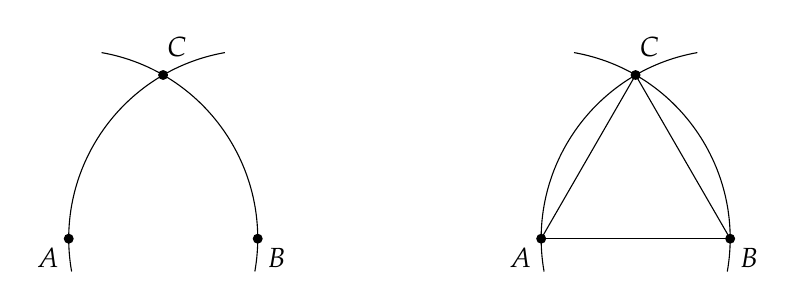
\begin{tikzpicture}[scale=0.6]
\coordinate (A) at (0,0);
\coordinate (B) at (4,0);
\path (A) node[below left] {$A$} -- (B) node[below right] {$B$};
\fill (A) circle[radius=3pt];
\fill (B) circle[radius=3pt];
\draw[name path=larc] (A) ++(-10:4cm) arc (-10:80:4cm);
\draw[name path=rarc] (B) ++(-170:4cm) arc (-170:-260:4cm);
\path [name intersections={of=larc and rarc,by={t}}];
\fill (t) node[above right,xshift=-2pt,yshift=3pt] {$C$} circle[radius=3pt];
\begin{scope}[xshift=10cm]
\coordinate (A) at (0,0);
\coordinate (B) at (4,0);
\draw (A) node[below left] {$A$} -- (B) node[below right] {$B$};
\fill (A) circle[radius=3pt];
\fill (B) circle[radius=3pt];
\draw[name path=larc] (A) ++(-10:4cm) arc (-10:80:4cm);
\draw[name path=rarc] (B) ++(-170:4cm) arc (-170:-260:4cm);
\path [name intersections={of=larc and rarc,by={t}}];
\fill (t) node[above right,xshift=-2pt,yshift=3pt] {$C$} circle[radius=3pt];
\draw (A) -- (t);
\draw (B) -- (t);
\end{scope}
\end{tikzpicture}
\end{center}
In the diagrams we will draw lines, but they are used only to understand the construction and the proof of its correctness. It is important that you convince yourself that the construction itself uses only a compass.

Every step of a construction with straightedge and compass consists of one of the following three operations:
\begin{itemize}
\item Finding the point of intersection of two straight lines.
\item Finding the point of intersection of a straight line and a circle.
\item Finding the point(s) of intersection of two circles.
\end{itemize}
It is clear that the third operation can be done with only a compass. We need to show that the first two operations can be done with a compass alone.

Notation:
\begin{itemize}
\item $C(O,A)$: the circle with center $O$ through point $A$.
\item $C(O,r)$: the circle with center $O$ and radius $r$.
\item $C(O,AB)$: the circle with center $O$ and radius the length of line segment $AB$.
\end{itemize}

First we will solve four preliminary problems (Sections~\ref{s.reflection}--\ref{s.three}) and then we show the construction for finding the intersection of two lines (Section~\ref{s.two-lines}) and that of a line and a circle (Section~\ref{s.line-circle}).

%%%%%%%%%%%%%%%%%%%%%%%%%%%%%%%%%%%%%%%%%%%%%%%%%%%%%%%%%%%%%%%

\section{Reflection of a point}\label{s.reflection}

\textbf{Given a line $AB$ and a point $C$ not on $AB$, it is possible to build a point $C'$ which is a reflection of $C$ about $AB$.} $C'$ is a \emph{reflection} about a line segment $AB$ if $AB$ (or the line containing $AB$ is the perpendicular bisector of the line $CC'$.

We build a circle centered on $A$ passing through $C$ and circle centered on $B$ passing through $C$. The intersection of the two circles is the point $C'$ which is the reflection of $C$.
\begin{center}
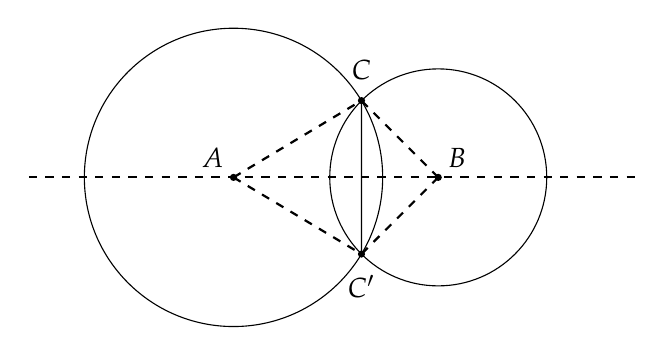
\begin{tikzpicture}[scale=.65]
\coordinate (A) at (0,0);
\coordinate (B) at (4,0);
\coordinate (C) at (2.5,1.5);
\draw[thick,dashed] ($(B)!2!(A)$) -- ($(A)!2!(B)$);
\fill (A) node[above left] {$A$} circle[radius=2pt];
\fill (B) node[above right] {$B$} circle[radius=2pt];
\fill (C) node[above,yshift=4pt] {$C$} circle[radius=2pt];
\node[draw,circle through=(C),name path=ac] at (A) {};
\node[draw,circle through=(C),name path=bc] at (B) {};
\path [name intersections={of=ac and bc,by={x1,Cp}}];
\fill (Cp) node[below,yshift=-4pt] {$C'$} circle[radius=2pt];
\draw (C) -- (Cp);
\draw[thick,dashed] (A) -- (C);
\draw[thick,dashed] (B) -- (C);
\draw[thick,dashed] (A) -- (Cp);
\draw[thick,dashed] (B) -- (Cp);
\end{tikzpicture}
\end{center}
\textbf{Proof:} $\triangle ABC \cong \triangle ABC'$ by SSS since $AC,AC'$ are radii of the same circle as are $BC,BC'$, and $AB$ is a common side. Therefore, $\angle CAB = \angle C'AB$ so $AB$ is the angle bisector of $\angle CAC'$. But $\triangle CAC'$ is an isosceles triangle and the angle bisector $AB$ is also the perpendicular bisector of the base of the triangle $CC'$. By definition $C'$ is the reflection of $C$ around $AB$.

%%%%%%%%%%%%%%%%%%%%%%%%%%%%%%%%%%%%%%%%%%%%%%%%%%%%%%%%%%%%%%%

\section{Construct a circle with a given radius}\label{s.circle}

\textbf{Given points $A,B,C$, construct$c(A,BC)$.}

Construct $c(A,B)$ and $c(B,A)$ and let $X$ and $Y$ be their points of intersection.

\begin{center}
\begin{tikzpicture}[scale=.55]
\coordinate (A) at (0,1.5);
\coordinate (B) at (0,-1.5);
\coordinate (C) at (1.5,-3);
\coordinate (Cp) at (1.5,3);
\fill (A) node[above] {$A$} circle[radius=3pt];
\fill (B) node[below] {$B$} circle[radius=3pt];
\fill (C) node[below] {$C$} circle[radius=3pt];
%\fill (Cp) node[above] {$C'$} circle[radius=3pt];
\node[draw,circle through=(B),name path=ab] at (A) {};
\node[draw,circle through=(A),name path=ba] at (B) {};
\path [name intersections={of=ab and ba,by={Y,X}}];
\fill (X) node[above right,xshift=4pt] {$X$} circle[radius=3pt];
\fill (Y) node[above left,xshift=-4pt] {$Y$} circle[radius=3pt];
\draw[thick,dashed] ($(X)!2.3!(Y)$) -- ($(Y)!2!(X)$);
\end{tikzpicture}
\vspace*{-6pt}
\end{center}
Construct $C'$, the reflection of $C$ about line $XY$ as described in Section~\ref{s.reflection}.

\begin{center}
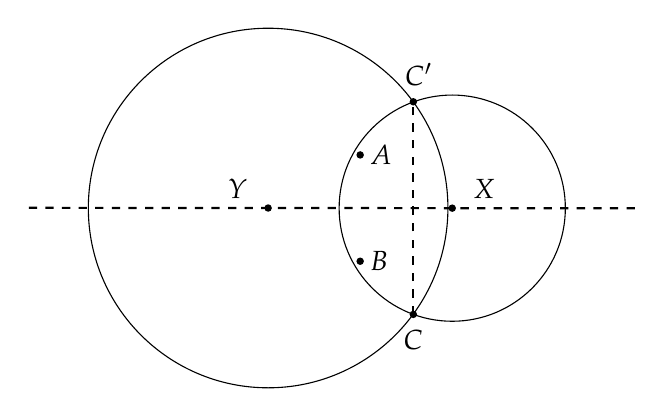
\begin{tikzpicture}[scale=.45]
\coordinate (A) at (0,1.5);
\coordinate (B) at (0,-1.5);
\coordinate (C) at (1.5,-3);
\coordinate (Cp) at (1.5,3);
\fill (A) node[right] {$A$} circle[radius=3pt];
\fill (B) node[right] {$B$} circle[radius=3pt];
\fill (C) node[below,yshift=-2pt] {$C$} circle[radius=3pt];
\fill (Cp) node[above,xshift=2pt,yshift=2pt] {$C'$} circle[radius=3pt];
\node[circle through=(B),name path=ab] at (A) {};
\node[circle through=(A),name path=ba] at (B) {};
\path [name intersections={of=ab and ba,by={Y,X}}];
\fill (X) node[above right,xshift=4pt] {$X$} circle[radius=3pt];
\fill (Y) node[above left,xshift=-4pt] {$Y$} circle[radius=3pt];
\node[draw,circle through=(C)] at (X) {};
\node[draw,circle through=(C)] at (Y) {};
\draw[thick,dashed] ($(X)!2.3!(Y)$) -- ($(Y)!2!(X)$);
%\draw (X) -- (Y) -- (C) -- (X) -- (Cp) -- (Y);
\draw[thick,dashed] (C) -- (Cp);
\end{tikzpicture}
\vspace*{-6pt}
\end{center}

$c(A,C')$ is the desired circle.

\begin{center}
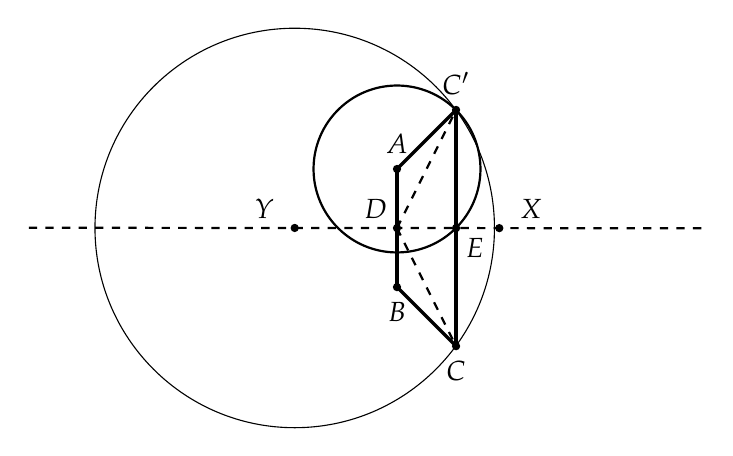
\begin{tikzpicture}[scale=.5]
\coordinate (A) at (0,1.5);
\coordinate (B) at (0,-1.5);
\coordinate (C) at (1.5,-3);
\coordinate (Cp) at (1.5,3);
\fill (A) node[above,yshift=2pt] {$A$} circle[radius=3pt];
\fill (B) node[below,yshift=-2pt] {$B$} circle[radius=3pt];
\fill (C) node[below,yshift=-2pt] {$C$} circle[radius=3pt];
\fill (Cp) node[above,yshift=2pt] {$C'$} circle[radius=3pt];
\node[circle through=(B),name path=ab] at (A) {};
\node[circle through=(A),name path=ba] at (B) {};
\path [name intersections={of=ab and ba,by={Y,X}}];
\fill (X) node[above right,xshift=4pt] {$X$} circle[radius=3pt];
\fill (Y) node[above left,xshift=-4pt] {$Y$} circle[radius=3pt];
\node[circle through=(C)] at (X) {};
\node[draw,circle through=(C)] at (Y) {};
\draw[thick,dashed] ($(X)!2.3!(Y)$) -- ($(Y)!2!(X)$);
\path[name path=xy] (X) -- (Y);
\node[draw,thick,circle through=(Cp)] at (A) {};
\draw[very thick] (A) -- (Cp);
\draw[very thick] (B) -- (C);
\draw[very thick,name path=abline] (A) -- (B);
\draw[very thick,name path=ccp] (C) -- (Cp);
\path [name intersections={of=xy and abline,by={D}}];
\path [name intersections={of=xy and ccp,by={E}}];
\fill (D) node[above left] {$D$} circle[radius=3pt];
\fill (E) node[below right] {$E$} circle[radius=3pt];
\draw[thick,dashed] (D) -- (Cp);
\draw[thick,dashed] (D) -- (C);
\end{tikzpicture}
\vspace*{-4pt}
\end{center}

\textbf{Proof:} $A$ is the reflection of $B$ around $XY$ (since $\triangle YAX\cong \triangle YBX$) and $C'$ is the reflection of $C$ around the $XY$. By definition, $XY$ is the perpendicular bisector of $CC'$ and $AB$, so $C'E=EC$, $AD=DB$ and $\angle DEC=\angle DEC'(=90^\circ)$. $\triangle DEC\cong\triangle DEC'$ by SAS, so $DC=DC'$ and $\angle ADC'=\angle BDC$ (they are complementary to $\angle EDC'$, $\angle EDC$). Therefore, $\triangle ADC'\cong\triangle BDC$ by ASA, so $AC'=BC$.

%%%%%%%%%%%%%%%%%%%%%%%%%%%%%%%%%%%%%%%%%%%%%%%%%%%%%%%%%%%%%%%

\section{Addition and subtraction of line segments}\label{s.add-subtract}

\textbf{Given line segment $PQ$ of length $a$ and line segment $RS$ of length $b$, it is possible to construct line segments $QT,QU$ such that $PUQT$ is a line segment, where the length of $PU$ is $a-b$ and the length of $PT$ is $a+b$.}
\begin{center}
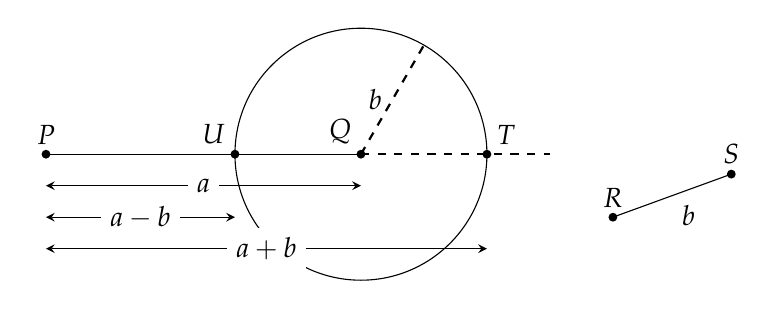
\begin{tikzpicture}[scale=.8]
\draw (0,0) -- (5,0);
\fill (0,0) node[above] {$P$} circle[radius=2pt];
\fill (5,0) node[above left] {$Q$} circle[radius=2pt];
\fill (3,0) node[above left] {$U$} circle[radius=2pt];
\fill (7,0) node[above right] {$T$} circle[radius=2pt];
\draw[thick,dashed] (5,0) -- (8,0);
\draw (5,0) circle[radius=2cm];
\draw[thick,dashed] (5,0) -- node[left] {$b$} ++(60:2cm);
\draw (9,-1) node[above] {$R$} -- node[below right] {$b$} ++(20:2cm) node[above] {$S$};
\fill (9,-1) circle[radius=2pt];
\fill (9,-1) ++(20:2cm) circle[radius=2pt];
\draw[<->] (0,-.5) -- node[fill=white] {$a$} (5,-.5);
\draw[<->] (0,-1) -- node[fill=white] {$a-b$} (3,-1);
\draw[<->] (0,-1.5) -- node[fill=white] {$a+b$} (7,-1.5);
\end{tikzpicture}
\end{center}

\newpage

\subsection*{Constructing an isosceles trapezoid}

Let $H$ be any point on $c(Q,b)$. Construct $H'$, its reflection about $PQ$. $h$ is the length of $HH'$:

\vspace{-1ex}

\begin{center}
\begin{tikzpicture}[scale=.6]
\coordinate (Q) at (0,0);
\coordinate (P) at (-6.8,0);
\coordinate (B) at (-3,-2);
\draw[thick,dashed] ($(Q)!1.3!(P)$) -- node[above,near start] {$a$} ($(P)!2.3!(Q)$);
\fill (Q) node[above left] {$Q$} circle[radius=2pt];
\fill (P) node[above] {$P$} circle[radius=2pt];
\fill (B) circle[radius=2pt];
\node[draw,circle through=(B),name path=qb] at (Q) {};
\draw[thick,dashed] (Q) -- node[left,xshift=-1pt,yshift=2pt] {$b$} (B);
\path[name path=qh] (Q) -- (-40:5cm);
\path[name path=qhp] (Q) -- (40:5cm);
\path [name intersections={of=qb and qh,by={H}}];
\path [name intersections={of=qb and qhp,by={Hp}}];
\fill[below right] (H) node[right,xshift=2pt] {$H$} circle[radius=2pt];
\fill[above right] (Hp) node[right,xshift=2pt] {$H'$} circle[radius=2pt];
\draw[thick,dashed] (H) -- node[below left,yshift=-2pt] {$h$} (Hp);
\end{tikzpicture}
\end{center}

\vspace{-2ex}

Construct the circles $C(H,b)$, $c(Q,h)$. $K$ is the intersection of the circles and $K'$ be the reflection of $K$ about line $PQ$:

\begin{center}
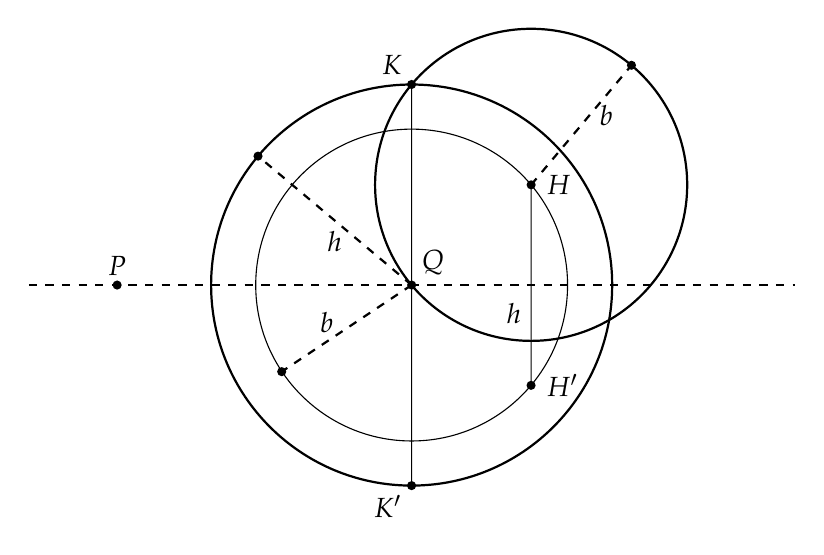
\begin{tikzpicture}[scale=.55]
\coordinate (Q) at (0,0);
\coordinate (P) at (-6.8,0);
\coordinate (B) at (-3,-2);
\draw[thick,dashed] ($(Q)!1.3!(P)$) -- ($(P)!2.3!(Q)$);
\fill (Q) node[above right] {$Q$} circle[radius=3pt];
\fill (P) node[above] {$P$} circle[radius=3pt];
\fill (B) circle[radius=3pt];
\node[draw,circle through=(B),name path=qb] at (Q) {};
\draw[thick,dashed] (Q) -- node[left,xshift=-1pt,yshift=2pt] {$b$} (B);
\path[name path=qh] (Q) -- (-40:5cm);
\path[name path=qhp] (Q) -- (40:5cm);
\path [name intersections={of=qb and qh,by={Hp}}];
\path [name intersections={of=qb and qhp,by={H}}];
\fill (H) node[right,xshift=2pt] {$H$} circle[radius=3pt];
\fill (Hp) node[right,xshift=2pt] {$H'$} circle[radius=3pt];
\draw (H) -- node[below left,yshift=-3pt] {$h$} (Hp);
\draw[thick,name path=circleqh] (Q) let
  \p1 = ($ (H) - (Hp) $),
  \n2 = {veclen(\x1,\y1)}
in
  circle (\n2)
  (Q) edge [dashed] node[below] {$h$} +(140:\n2) ++(140:\n2) coordinate (q);
\fill (q) circle[radius=3pt];
\draw[thick,name path=circlehb] (H) let
  \p1 = ($ (Q) - (B) $),
  \n2 = {veclen(\x1,\y1)}
in
  circle (\n2)
  (H) edge [dashed] node[below,near end] {$b$} +(50:\n2) ++(50:\n2)  coordinate (h);
\fill (h) circle[radius=3pt];
\path [name intersections={of=circleqh and circlehb,by={K}}];
\fill (K) node[above left] {$K$} circle[radius=3pt];
%\draw[thick] (H) -- (K);
\draw let
  \p1 = ($ (K) - (Q) $)
in
  coordinate (Kp) at (\x1,-\y1);
\fill (Kp) node[below left] {$K'$} circle[radius=3pt];
\draw (K) -- (Kp);
\end{tikzpicture}
\vspace*{-8pt}
\end{center}

$PQ$ is the perpendicular bisector of both $HH'$ and $KK'$, so these line segments are parallel. $KH=K'H'=b$ since both are radii of the circle centered on $H$. $K',H'$ are reflections of $K,H$. Therefore, $KHH'K'$ is an isosceles trapezoid whose bases are $HH'=h$, $KK'=2h$. Label $d$, the length of the diagonals $K'H=KH'$:


\begin{center}
\vspace*{-8pt}
\begin{tikzpicture}[scale=.6]
\coordinate (Q) at (0,0);
\coordinate (P) at (-6.8,0);
\coordinate (B) at (-3,-2);
\draw[thick,dashed] ($(Q)!1.3!(P)$) -- ($(P)!2.3!(Q)$);
\fill (Q) node[above left] {$Q$} circle[radius=3pt];
\fill (P) node[above] {$P$} circle[radius=3pt];
%\fill (B) circle[radius=3pt];
\node[draw,circle through=(B),name path=qb] at (Q) {};
%\draw[thick,dashed] (Q) -- node[left,xshift=-1pt,yshift=2pt] {$b$} (B);
\path[name path=qh] (Q) -- (-40:5cm);
\path[name path=qhp] (Q) -- (40:5cm);
\path [name intersections={of=qb and qh,by={Hp}}];
\path [name intersections={of=qb and qhp,by={H}}];
\fill (H) node[right,xshift=2pt] {$H$} circle[radius=3pt];
\fill (Hp) node[right,xshift=2pt] {$H'$} circle[radius=3pt];
\draw (H) -- node[below right,yshift=-2pt] {$h$} (Hp);
\path[name path=circleqh] (Q) let
  \p1 = ($ (H) - (Hp) $)
in
  circle ({veclen(\x1,\y1)});
\path[name path=circlehb] (H) let
  \p1 = ($ (Q) - (B) $)
in
  circle ({veclen(\x1,\y1)});
\path [name intersections={of=circleqh and circlehb,by={K,k2}}];
\fill (K) node[above left] {$K$} circle[radius=3pt];
\draw (Q) -- node[left] {$h$} (K);
\draw (H) -- node[right,xshift=4pt] {$b$} (K);
\draw let
  \p1 = ($ (K) - (Q) $)
in
  coordinate (Kp) at (\x1,-\y1);
\fill (Kp) node[below left] {$K'$} circle[radius=3pt];
\draw (Q) -- node[left] {$h$} (Kp) -- node[right,xshift=2pt,yshift=-2pt] {$b$} (Hp);
\draw (K) -- node[above right] {$d$} (Hp);
\draw (Kp) -- node[left] {$d$} (H);
\end{tikzpicture}
\label{ptolemy}
\vspace*{-8pt}
\end{center}

\subsection*{Circumscribing the trapezoid by a circle}

We want to proof that it is possible to circumscribe $KHH'K'$ by a circle. We prove that is the opposite angles of a quadrilateral are supplementary, then the trapezoid can be circumscribed by a circle, and we proof that in an isosceles trapezoid the opposite angles are supplementary.

Geometry textbooks give the simple proof that the opposite angles of a quadrilateral circumscribed by a circle are supplementary, but it is hard to find a proof of the converse, so I present both proofs here.

\textbf{If a quadrilateral can be circumscribed by a circle then the opposite angles are supplementary:} An inscribed angle equals half the subtended arc, so $\angle DAB$ is half of the arc $DCB$ and $\angle DCB$ is half of the arc $DAB$. The two arcs subtend the entire circumference of the circle, so their sum is $360^\circ$. Therefore, $\angle DAB + \angle DCB = \disfrac{1}{2} \cdot 360^\circ =  180^\circ$, and similarly $\angle ADC + \angle AABC = 180^\circ$

\vspace*{-2ex}

\begin{center}
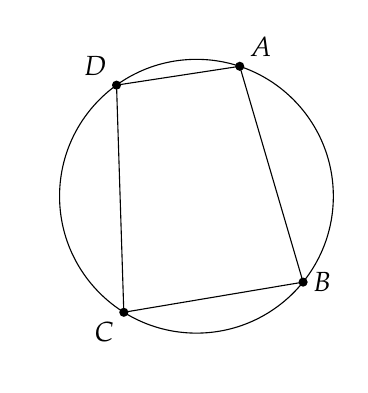
\begin{tikzpicture}[scale=.55]
\coordinate (origin) at (0,0);
\coordinate (A) at (1,3);
\node[draw,circle through=(A),name path=circle] at (origin) {};
\fill (A) node[above right] {$A$} circle[radius=3pt];
\path[name path=b] (A) -- (-50:4.5cm);
\path[name path=c] (A) -- (-120:4.5cm);
\path[name path=d] (A) -- (150:4.5cm);
\path [name intersections={of=circle and b,by={b1,B}}];
\fill (B) node[right] {$B$} circle[radius=3pt];
\path [name intersections={of=circle and c,by={c1,C}}];
\fill (C) node[below left] {$C$} circle[radius=3pt];
\path [name intersections={of=circle and d,by={d1,D}}];
\fill (D) node[above left] {$D$} circle[radius=3pt];
\draw (A) -- (B) -- (C) -- (D) -- cycle;
\end{tikzpicture}
\end{center}

\vspace*{-2ex}

\textbf{Quadrilateral whose opposite angles are supplementary can be circumscribed by a circle:} Any triangle can be circumscribed by a circle. Circumscribed $\triangle DAB$ by a circle and suppose that $C'$ is a point such that $\angle DAB + \angle DC'B = 180^\circ$, but $C'$ is \emph{not} on the circumference of the circle. Without loss of generality, let $C'$ be within the circle:

\vspace*{-1ex}

\begin{center}
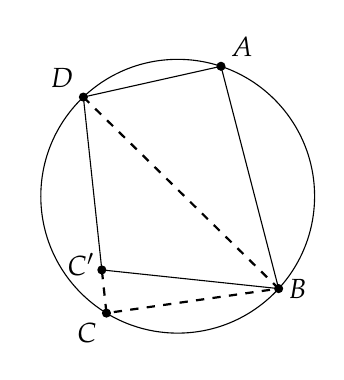
\begin{tikzpicture}[scale=.55]
\coordinate (origin) at (0,0);
\coordinate (A) at (1,3);
\node[draw,circle through=(A),name path=circle] at (origin) {};
\fill (A) node[above right] {$A$} circle[radius=3pt];
\path[name path=b] (A) -- (-50:4cm);
\path[name path=c] (A) -- (-120:4cm);
\path[name path=d] (A) -- (150:4cm);
\path [name intersections={of=circle and b,by={b1,B}}];
\fill (B) node[right] {$B$} circle[radius=3pt];
\path [name intersections={of=circle and c,by={c1,C}}];
\fill (C) node[below left] {$C$} circle[radius=3pt];
\path [name intersections={of=circle and d,by={d2,D}}];
\fill (D) node[above left] {$D$} circle[radius=3pt];
\coordinate (Cp) at ($(C)!.2!(D)$);
\draw (A) -- (B) -- (Cp) -- (D) -- cycle;
\fill (Cp) node[left,xshift=1pt,yshift=2pt] {$C'$} circle[radius=3pt];
\draw[thick,dashed] (D) -- (B) -- (C) -- (Cp);
\end{tikzpicture}
\end{center}

\vspace*{-1ex}

Construct a ray that extends $DC'$ and let $C$ be its intersection with the circle. $ABCD$ is circumscribed by a circle so:
\begin{eqnarray*}
\angle DAB + \angle DCB &=& 180^\circ\\
\angle DAB + \angle DCB &=& \angle DAB + \angle DC'B\\
\angle DCB &=& \angle DC'B\,,
\end{eqnarray*}
which is impossible if $C$ is on the circle and $C'$ is inside the circle.

Finally, we show that the opposite angles of an isosceles trapezoid are supplementary.

\begin{center}
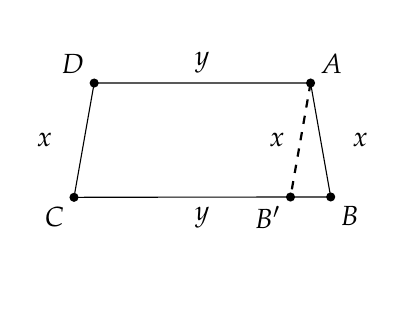
\begin{tikzpicture}[scale=.55]
\coordinate (origin) at (0,0);
\coordinate (A) at (2.5,1.8);
\node[circle through=(A),name path=circle] at (origin) {};
\fill (A) node[above right] {$A$} circle[radius=3pt];
\path[name path=b] (A) -- ++(-80:4cm);
\path[name path=d] (A) -- ++(180:6cm);
\path [name intersections={of=circle and b,by={b1,B}}];
\fill (B) node[below right] {$B$} circle[radius=3pt];
\path [name intersections={of=circle and d,by={d1,D}}];
\fill (D) node[above left] {$D$} circle[radius=3pt];
\path[name path=c] (D) -- ++(-100:4cm);
\path [name intersections={of=circle and c,by={c1,C}}];
\fill (C) node[below left] {$C$} circle[radius=3pt];
\draw (A) -- node[right,xshift=8pt] {$x$} (B);
\draw[name path=bc] (B) -- node[below] {$y$} (C);
\draw (C) -- node[left,xshift=-8pt] {$x$} (D) -- node[above] {$y$} (A);
\path[name path=para] (A) -- ++(-100:4cm);
\path [name intersections={of=para and bc,by={Bp}}];
\fill (Bp) node[below left] {$B'$} circle[radius=3pt];
\draw[thick,dashed] (A) -- node[left,xshift=-2pt] {$x$} (Bp);
\end{tikzpicture}
\end{center}

\vspace{-4ex}

Construct the line $AB'$ parallel to $CD$. $AB'CD$ is a parallelogram and $\triangle ABB'$ is an isosceles triangle, so $\angle C= \angle ABB' = \angle AB'B = \angle B$. Similarly, $\angle A = \angle D$. Since the sum of the internal angles of any quadrilateral is equal to $360^\circ$:
\begin{eqnarray*}
\angle A + \angle B + \angle C + \angle D &=& 360^\circ\\
2\angle A + 2 \angle C &=& 360^\circ\\
\angle A +  \angle C &=& 180^\circ\,.
\end{eqnarray*}
and similarly $\angle B +  \angle D = 180^\circ$.

\subsection*{Ptolemy's theorem}

We will use Ptolemy's theorem, an equation which relates the lengths of the diagonals and the lengths of the sides of a quadrilateral that is circumscribed by a circle:
\[
ef = ac + bd\,.
\]
\begin{center}
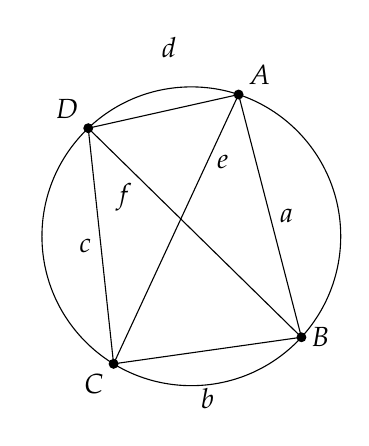
\begin{tikzpicture}[scale=.6]
\coordinate (origin) at (0,0);
\coordinate (A) at (1,3);
\node[draw,circle through=(A),name path=circle] at (origin) {};
\fill (A) node[above right] {$A$} circle[radius=3pt];
\path[name path=b] (A) -- (-50:4cm);
\path[name path=c] (A) -- (-120:4cm);
\path[name path=d] (A) -- (150:4cm);
\path [name intersections={of=circle and b,by={b1,B}}];
\fill (B) node[right] {$B$} circle[radius=3pt];
\path [name intersections={of=circle and c,by={C,c2}}];
\fill (C) node[below left] {$C$} circle[radius=3pt];
\path [name intersections={of=circle and d,by={D,d2}}];
\fill (D) node[above left] {$D$} circle[radius=3pt];
\draw (A) -- node[right] {$a$} (B) -- node[below,yshift=-10pt] {$b$} (C) -- node[left] {$c$} (D) -- node[above,xshift=2pt,yshift=16pt] {$d$}  cycle;
\draw (A) -- node[right,near start] {$e$} (C);
\draw (B) -- node[left,near end,yshift=-6pt] {$f$} (D);
\end{tikzpicture}
\end{center}
There is a geometric proof of the theorem (see Wikipedia), but I will present a simple trigonometric proof. The law of cosines for the four triangles $\triangle ABC$, $\triangle ADC$, $\triangle DAB$, $\triangle DCB$ gives the following equations:
\begin{eqnarray*}
e^2 &=& a^2 + b^2 - 2ab \cos \angle B\\
e^2 &=& c^2 + d^2 - 2cd \cos \angle D\\
f^2 &=& a^2 + d^2 - 2ad \cos \angle A\\
f^2 &=& b^2 + c^2 - 2bc \cos \angle C\,.
\end{eqnarray*}
$\angle C = 180^\circ - \angle A$ and $\angle D = 180^\circ - \angle B$ because they are opposite angles of a quadrilateral circumscribed by a circle, so:
\begin{eqnarray*}
\cos \angle D &=& - \cos \angle B\\
\cos \angle C &=& -\cos \angle A\,.
\end{eqnarray*}
We can eliminate the cosine term from the first two equations and from the last two equations. After some messy arithmetic, we get:
\begin{eqnarray*}
e^2 &=& \frac{(ac+bd)(ad+bc)}{(ab+cd)}\\
f^2 &=& \frac{(ab+cd)(ac+bd)}{(ad+bc)}\,.
\end{eqnarray*}
Multiply the two equations and simplify to get Ptolemy's theorem:
\begin{eqnarray*}
e^2\cdot f^2 &=& (ac+bd)^2\\
ef &=& (ac+bd)\,. 
\end{eqnarray*}
\subsection*{Using Ptolemy's theorem}

For the construction on page~\pageref{ptolemy}, the diagonals are of length $d$, the legs are of length $b$, and the bases are of lengths $h$ and $2h$, so Ptolemy's theorem gives $d\cdot d = b\cdot b + h\cdot 2h$ or $d^2=b^2+2h^2$.

Let $X$ be the point on line $PQ$ that extends $PQ$ by $b$. (We will eventually construct $X$; now we're just imagining it.) Define  $x = K'X$. Since $\triangle QK'X$ is a right triangle, $x^2 = b^2 + h^2$:
\begin{center}
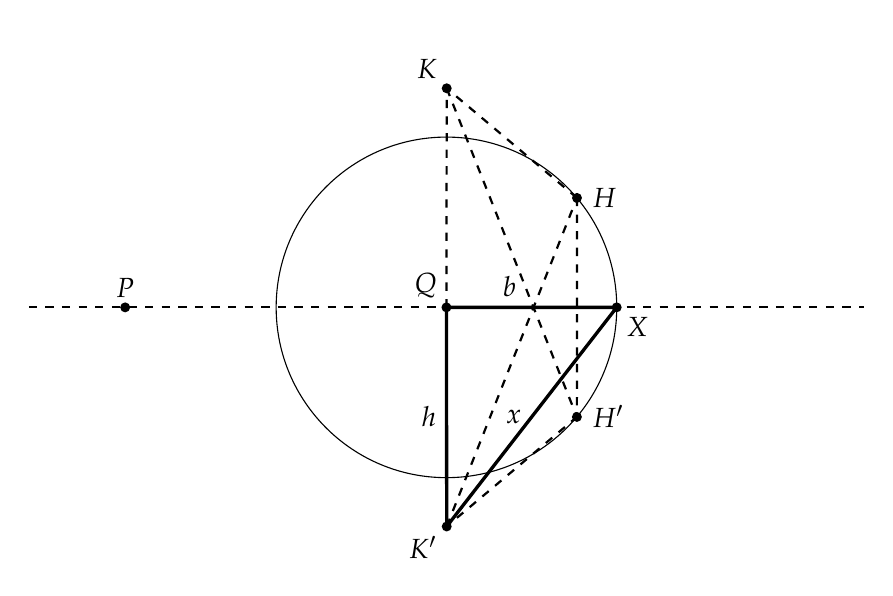
\begin{tikzpicture}[scale=.6]
\coordinate (Q) at (0,0);
\coordinate (P) at (-6.8,0);
\coordinate (B) at (-3,-2);
\draw[thick,dashed,name path=pq] ($(Q)!1.3!(P)$) -- ($(P)!2.3!(Q)$);
\fill (Q) node[above left] {$Q$} circle[radius=3pt];
\fill (P) node[above] {$P$} circle[radius=3pt];
%\fill (B) circle[radius=2pt];
\node[draw,circle through=(B),name path=qb] at (Q) {};
%\draw[thick,dashed] (Q) -- node[left,xshift=-1pt,yshift=2pt] {$b$} (B);
\path[name path=qh] (Q) -- (-40:5cm);
\path[name path=qhp] (Q) -- (40:5cm);
\path [name intersections={of=qb and qh,by={hp}}];
\path [name intersections={of=qb and qhp,by={H}}];
\fill (H) node[right,xshift=2pt] {$H$} circle[radius=3pt];
\fill (hp) node[right,xshift=2pt] {$H'$} circle[radius=3pt];
\draw[thick,dashed] (H) -- (hp);
\path[name path=circleqh] (Q) let
  \p1 = ($ (H) - (hp) $)
in
  circle ({veclen(\x1,\y1)});
\path[name path=circlehb] (H) let
  \p1 = ($ (Q) - (B) $)
in
  circle ({veclen(\x1,\y1)});
\path [name intersections={of=circleqh and circlehb,by={K,k2}}];
\fill (K) node[above left] {$K$} circle[radius=3pt];
\draw[thick,dashed] (Q) -- (K);
\draw[thick,dashed] (H) -- (K);
\draw[thick,dashed] let
  \p1 = ($ (K) - (Q) $)
in
  coordinate (kp) at (\x1,-\y1);
\fill (kp) node[below left] {$K'$} circle[radius=3pt];
\draw[thick,dashed] (Q) -- node[left] {$h$} (kp) -- (hp);
\draw[thick,dashed] (K) -- (hp);
\draw[thick,dashed] (kp) -- (H);
\path [name intersections={of=pq and qb,by={X,x2}}];
\fill (X) node[below right] {$X$} circle[radius=3pt];
\draw[thick,dashed] (kp) -- node[left] {$x$} (X);
\draw[very thick] (Q) -- (kp) -- (X) -- node[above,xshift=-8pt] {$b$} cycle;
\end{tikzpicture}
\vspace*{-8pt}
\end{center}
By Ptolemy's theorem:
\erh{0pt}
\begin{equationarray*}{rcl}
d^2&=&b^2 + 2h^2\\
&=&(x^2-h^2)+2h^2\\
&=&x^2+h^2\,.
\end{equationarray*}
Don't look for a right triangle in the diagram. We are claiming that \emph{it is possible to construct} the triangle with sides $x,h,d$. 

Let us construct the point $S$ as the intersection of the circles 
$c(K,d),c(K',d)$:
\begin{center}
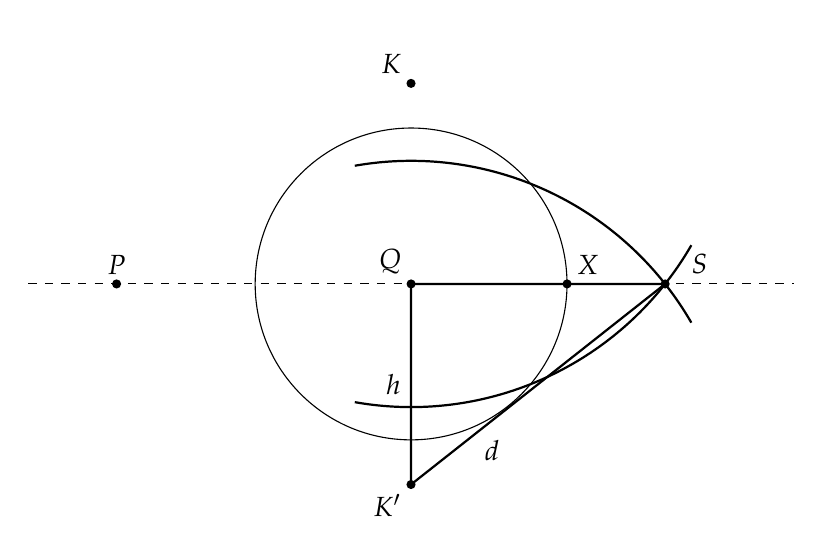
\begin{tikzpicture}[scale=.55]
\coordinate (Q) at (0,0);
\coordinate (P) at (-6.8,0);
\coordinate (B) at (-3,-2);
\draw[dashed,name path=pq] ($(Q)!1.3!(P)$) -- ($(P)!2.3!(Q)$);
\fill (Q) node[above left] {$Q$} circle[radius=3pt];
\fill (P) node[above] {$P$} circle[radius=3pt];
\node[draw,circle through=(B),name path=qb] at (Q) {};
\path[name path=qh] (Q) -- (-40:5cm);
\path[name path=qhp] (Q) -- (40:5cm);
\path [name intersections={of=qb and qh,by={Hp}}];
\path [name intersections={of=qb and qhp,by={H}}];
%\fill (H) node[right,xshift=2pt] {$H$} circle[radius=3pt];
%\fill (Hp) node[right,xshift=2pt] {$H'$} circle[radius=3pt];
\path[name path=circleqh] (Q) let
  \p1 = ($ (H) - (Hp) $)
in
  circle ({veclen(\x1,\y1)});
\path[name path=circlehb] (H) let
  \p1 = ($ (Q) - (B) $)
in
  circle ({veclen(\x1,\y1)});
\path [name intersections={of=circleqh and circlehb,by={K,k2}}];
\fill (K) node[above left] {$K$} circle[radius=3pt];
\draw[thick,dashed] let
  \p1 = ($ (K) - (Q) $)
in
  coordinate (Kp) at (\x1,-\y1);
\fill (Kp) node[below left] {$K'$} circle[radius=3pt];
\draw[thick] (Q) -- node[left] {$h$} (Kp);
\draw[thick,name path=khp] (K) let
  \p1 = ($ (H) - (Kp) $),
  \n2 = {veclen(\x1,\y1)}
in
  (K) ++(-100:\n2) arc (-100:-30:\n2);
\draw[thick,name path=kph] (Kp) let
  \p1 = ($ (H) - (Kp) $),
  \n2 = {veclen(\x1,\y1)}
in
  (Kp) ++(100:\n2) arc (100:30:\n2);
\path [name intersections={of=kph and khp,by={S}}];
\fill (S) node[above right,xshift=6pt] {$S$} circle[radius=3pt];
\draw[thick] (Kp) -- node[right,near start,yshift=-6pt] {$d$} (S);
\draw[thick] (Q) -- (S);
\path [name intersections={of=pq and qb,by={X,Xp}}];
\fill (X) node[above right] {$X$} circle[radius=3pt];
%\fill (Xp) node[above left] {$X'$} circle[radius=3pt];
%\draw (Kp) -- node[left] {$x$} (X);
%\draw (K) -- node[left] {$x$} (X);
%\fill (B) circle[radius=3pt];
%\draw[thick,dashed] (Q) -- node[left,xshift=-1pt,yshift=2pt] {$b$} (B);
\end{tikzpicture}
\end{center}
We obtain a right triangle $\triangle QSK'$. By Pythagoras' theorem 
$QS^2 + h^2 = d^2$, so:
\[
QS^2 = d^2-h^2=x^2\,,
\]
and $QS=x$.

It is possible to construct the point $X$ as the intersection of the circles $c(K,x),$:
\begin{center}
\vspace*{-14pt}
\begin{tikzpicture}[scale=.55]
\coordinate (Q) at (0,0);
\coordinate (P) at (-6.8,0);
\coordinate (B) at (-3,-2);
\draw[dashed,name path=pq] ($(Q)!1.3!(P)$) -- ($(P)!2.3!(Q)$);
\fill (Q) node[above left] {$Q$} circle[radius=3pt];
\fill (P) node[above] {$P$} circle[radius=3pt];
\node[draw,circle through=(B),name path=qb] at (Q) {};
\path[name path=qh] (Q) -- (-40:5cm);
\path[name path=qhp] (Q) -- (40:5cm);
\path [name intersections={of=qb and qh,by={Hp}}];
\path [name intersections={of=qb and qhp,by={H}}];
%\fill (H) node[right,xshift=2pt] {$H$} circle[radius=3pt];
%\fill (Hp) node[right,xshift=2pt] {$H'$} circle[radius=3pt];
\path[name path=circleqh] (Q) let
  \p1 = ($ (H) - (Hp) $)
in
  circle ({veclen(\x1,\y1)});
\path[name path=circlehb] (H) let
  \p1 = ($ (Q) - (B) $)
in
  circle ({veclen(\x1,\y1)});
\path [name intersections={of=circleqh and circlehb,by={K,k2}}];
\fill (K) node[above left] {$K$} circle[radius=3pt];
\path[thick,dashed] let
  \p1 = ($ (K) - (Q) $)
in
  coordinate (Kp) at (\x1,-\y1);
\fill (Kp) node[below left] {$K'$} circle[radius=3pt];
%\draw[thick] (Q) -- node[left] {$h$} (Kp);
\path[name path=khp] (K) let
  \p1 = ($ (H) - (Kp) $),
  \n2 = {veclen(\x1,\y1)}
in
  (K) ++(-100:\n2) arc (-100:-30:\n2);
\path[name path=kph] (Kp) let
  \p1 = ($ (H) - (Kp) $),
  \n2 = {veclen(\x1,\y1)}
in
  (Kp) ++(100:\n2) arc (100:30:\n2);
\path [name intersections={of=kph and khp,by={S}}];
\fill (S) node[above right,xshift=6pt] {$S$} circle[radius=3pt];
%\draw[thick] (Kp) -- node[right,near start,yshift=-6pt] {$d$} (S);
%\draw[thick] (Q) -- (S);
\path [name intersections={of=pq and qb,by={X,Xp}}];
\fill (X) node[above right,xshift=8pt] {$X$} circle[radius=3pt];
\fill (Xp) node[above left] {$X'$} circle[radius=3pt];
\draw (Kp) -- node[left] {$x$} (X);
\draw (K) -- node[left] {$x$} (X);
%\fill (B) circle[radius=3pt];
%\draw[thick,dashed] (Q) -- node[left,xshift=-1pt,yshift=2pt] {$b$} (B);
\draw[name path=kx] (K) let
  \p1 = ($ (X) - (Kp) $),
  \n2 = {veclen(\x1,\y1)}
in
  (K) ++(-100:\n2) arc (-100:-30:\n2);
\draw[name path=kpx] (Kp) let
  \p1 = ($ (X) - (Kp) $),
  \n2 = {veclen(\x1,\y1)}
in
  (Kp) ++(100:\n2) arc (100:30:\n2);
\path (Xp) -- node[below] {$b$} (Q);
\path (Q) -- node[below] {$b$} (X);
\node at (-5,2) {\mbox{\boldmath $PQ=a$}};
\draw[thick,dashed] (Q) -- node[left] {$h$} (Kp);
\draw[thick,dashed] (Q) -- (X);
\end{tikzpicture}
\vspace*{-10pt}
\end{center}
Recall that we want to extend $PQ$ of length $a$ by a length $b$, or decrease its length by $b$. Since the length of $QX$ is $\sqrt{x^2-h^2}=b$, the length of $PX$ is $a+b$ and the length of $PX'$ is $a-b$.

%%%%%%%%%%%%%%%%%%%%%%%%%%%%%%%%%%%%%%%%%%%%%%%%%%%%%%%%%%%%%%%

\section{Construction of a line segment whose length is defined relative to three other line segments}\label{s.three}

\textbf{Given line segments of length $n,m,s$ it is possible to construct a line segment of length $x = \disfrac{n}{m}s$.}

Construct two concentric circles $c_1 = c(Z,m)$ and $c_2 = c(Z,n)$, and chord $AB = s$ on $c_1$. (A chord can be constructed using only a compass as shown in Section~\ref{s.circle}.)

We assume that $m>n$. If not, exchange the notation.
\begin{center}
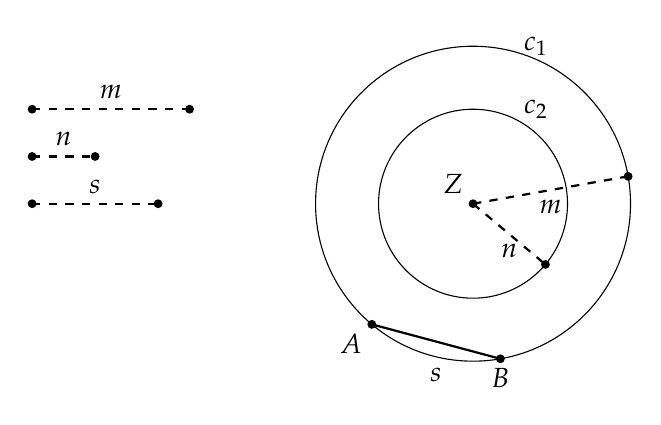
\begin{tikzpicture}[scale=.4]
\coordinate (Z) at (0,0);
\coordinate (A) at (-130:5cm);
\coordinate (B) at (-80:5cm);
\fill (Z) node[above left] {$Z$} circle[radius=4pt];
\fill (A) node[below left] {$A$} circle[radius=4pt];
\fill (B) node[below] {$B$} circle[radius=4pt];
\draw[name path=c1] (Z) circle[radius=5cm];
\draw[name path=c2] (Z) circle[radius=3cm];
\node at (2,5) {$c_1$};
\node at (2,3) {$c_2$};
\draw[thick] (A) -- node[below,yshift=-6pt] {$s$} (B);
\draw[thick,dashed] (Z) -- node[below] {$m$} ++(10:5cm);
\draw[thick,dashed] (Z) -- node[below] {$n$} ++(-40:3cm);
\fill (Z) ++ (10:5cm) circle[radius=4pt];
\fill (Z) ++ (-40:3cm) circle[radius=4pt];
\begin{scope}[xshift=-14cm,yshift=3cm]
\coordinate (m) at (0,0);
\coordinate (n) at (0,-1.5);
\coordinate (s) at (0,-3);
\coordinate (mp) at (5,0);
\coordinate (np) at (2,-1.5);
\coordinate (sp) at (4,-3);
\fill (m) circle[radius=4pt];
\fill (n) circle[radius=4pt];
\fill (s) circle[radius=4pt];
\fill (mp) circle[radius=4pt];
\fill (np) circle[radius=4pt];
\fill (sp) circle[radius=4pt];
\draw[thick,dashed] (m) -- node[above] {$m$} (mp);
\draw[thick,dashed] (n) -- node[above] {$n$} (np);
\draw[thick,dashed] (s) -- node[above] {$s$} (sp);
\end{scope}
\end{tikzpicture}
\end{center}

\vspace{-2ex}

We also assume that $s$ does not intersect $c_2$. If not, use the construction in Section~\ref{s.add-subtract} to multiply $m,n$ by a number $k$ so that the chord does not intersect the circle. Note that this does not change the value that we are trying to construct since $x=\disfrac{kn}{km}s=\disfrac{n}{m}s$.

Choose any point $H$ on circle $c_2$. Label the length of $AH$ by $w$. Construct point $K$ on $c_2$ such that the length of $BK$ is $w$.
\begin{center}
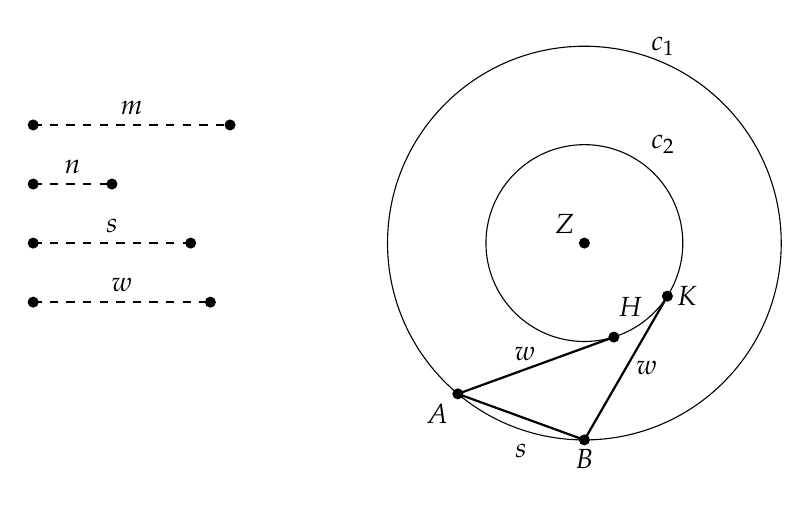
\begin{tikzpicture}[scale=.5]
\coordinate (Z) at (0,0);
\coordinate (A) at (-130:5cm);
\coordinate (B) at (-90:5cm);
\fill (Z) node[above left] {$Z$} circle[radius=4pt];
\fill (A) node[below left] {$A$} circle[radius=4pt];
\fill (B) node[below] {$B$} circle[radius=4pt];
\draw[name path=c1] (Z) circle[radius=5cm];
\draw[name path=c2] (Z) circle[radius=2.5cm];
\node at (2,5) {$c_1$};
\node at (2,2.5) {$c_2$};
\draw[thick] (A) -- node[below,yshift=-6pt] {$s$} (B);
\draw[thick] (A) -- node[above,xshift=-4pt,yshift=-2pt] {$w$} +(20:120pt) coordinate (H);
\fill (H) node[above right,xshift=-2pt,yshift=4pt] {$H$} circle[radius=4pt];
\draw[thick] (B) -- node[right] {$w$} +(60:120pt) coordinate (K);
\fill (K) node[right] {$K$} circle[radius=4pt];
\begin{scope}[xshift=-14cm,yshift=3cm]
\coordinate (m) at (0,0);
\coordinate (n) at (0,-1.5);
\coordinate (s) at (0,-3);
\coordinate (w) at (0,-4.5);
\coordinate (mp) at (5,0);
\coordinate (np) at (2,-1.5);
\coordinate (sp) at (4,-3);
\coordinate (wp) at (4.5,-4.5);
\fill (m) circle[radius=4pt];
\fill (n) circle[radius=4pt];
\fill (s) circle[radius=4pt];
\fill (w) circle[radius=4pt];
\fill (mp) circle[radius=4pt];
\fill (np) circle[radius=4pt];
\fill (sp) circle[radius=4pt];
\fill (wp) circle[radius=4pt];
\draw[thick,dashed] (m) -- node[above] {$m$} (mp);
\draw[thick,dashed] (n) -- node[above] {$n$} (np);
\draw[thick,dashed] (s) -- node[above] {$s$} (sp);
\draw[thick,dashed] (w) -- node[above] {$w$} (wp);
\end{scope}
\end{tikzpicture}
\end{center}

$\triangle AHZ\cong\triangle BZK$ by SSS: $ZA=ZB=m$, the radius of $c_1$, $ZH=ZK=n$, the radius of $c_2$, and $AH=BK=w$ by construction.

\begin{center}
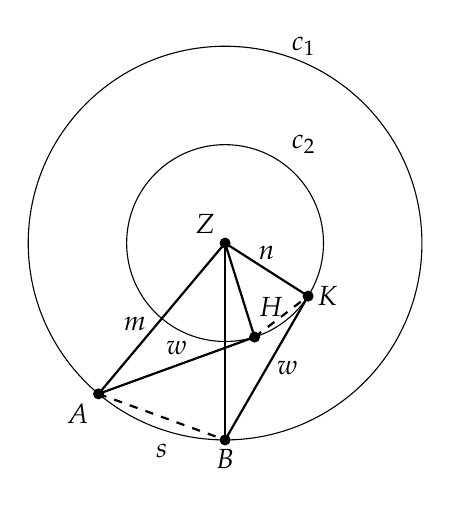
\begin{tikzpicture}[scale=.5]
\coordinate (Z) at (0,0);
\coordinate (A) at (-130:5cm);
\coordinate (B) at (-90:5cm);
\fill (Z) node[above left] {$Z$} circle[radius=4pt];
\fill (A) node[below left] {$A$} circle[radius=4pt];
\fill (B) node[below] {$B$} circle[radius=4pt];
\draw[name path=c1] (Z) circle[radius=5cm];
\draw[name path=c2] (Z) circle[radius=2.5cm];
\node at (2,5) {$c_1$};
\node at (2,2.5) {$c_2$};
\draw[thick,dashed] (A) -- node[below,yshift=-6pt] {$s$} (B);
\draw[thick] (A) -- node[above] {$w$} +(20:120pt) coordinate (H);
\fill (H) node[above right,xshift=-2pt,yshift=4pt] {$H$} circle[radius=4pt];
\draw[thick] (B) -- node[right] {$w$} +(60:120pt) coordinate (K);
\fill (K) node[right] {$K$} circle[radius=4pt];
\draw[thick] (Z) -- node[left,xshift=-2pt,yshift=-2pt] {$m$} (A);
\draw[thick] (Z) -- (B);
\draw[thick] (Z) -- (H);
\draw[thick] (Z) -- node[above] {$n$} (K);
\draw[thick,dashed] (H) -- (K);
\end{tikzpicture}
\end{center}
From $\triangle AHZ\cong\triangle BZK$, we get $\angle AZB = \angle HZK$. It is difficult to see this equality from the diagram, but the following diagram clarifies the relation among the angles. Define $\alpha = \angle AZH = \angle BZK$ and $\beta = \angle BZH$. It is easy to see that $\angle AZB = \angle HZK = \alpha - \beta$.
\begin{center}
\vspace*{-10pt}
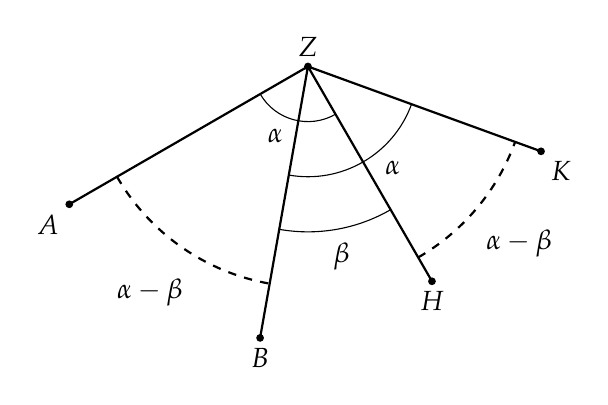
\begin{tikzpicture}[scale=.7]
\coordinate (Z) at (0,0);
\coordinate (A) at (-150:5cm);
\coordinate (B) at (-100:5cm);
\coordinate (H) at (-60:4.5cm);
\coordinate (K) at (-20:4.5cm);
\fill (Z) circle[radius=2pt];
\fill (A) circle[radius=2pt];
\fill (B) circle[radius=2pt];
\fill (H) circle[radius=2pt];
\fill (K) circle[radius=2pt];
\draw[thick] (A) node[below left] {$A$} -- (Z) node[above] {$Z$} -- (B) node[below] {$B$};
\draw[thick] (H) node[below] {$H$} -- (Z) -- (K) node[below right] {$K$};
\draw (-150:1cm) arc (-150:-60:1);
\draw (-100:2cm) arc (-100:-20:2);
\draw (-100:3cm) arc (-100:-60:3);
\draw[thick,dashed] (-150:4cm) arc (-150:-100:4);
\draw[thick,dashed] (-60:4cm) arc (-60:-20:4);
\node at (-115:1.4) {$\alpha$};
\node at (-50:2.4) {$\alpha$};
\node at (-80:3.5) {$\beta$};
\node at (-40:5) {$\alpha - \beta$};
\node at (-125:5) {$\alpha - \beta$};
\end{tikzpicture}
\vspace*{-10pt}
\end{center}

$\triangle ZAB\sim\triangle ZHK$ by SAS, since both are isosceles triangles and we have shown that they have the same vertex angle.

\vspace{-2ex}

\begin{center}
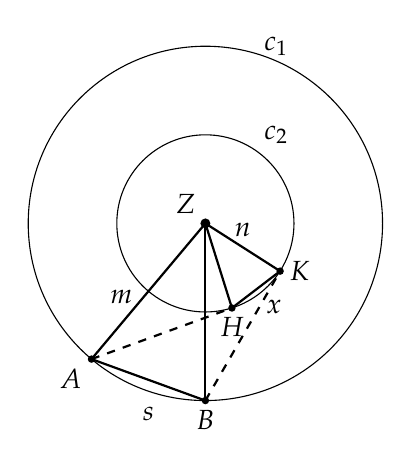
\begin{tikzpicture}[scale=.45]
\coordinate (Z) at (0,0);
\coordinate (A) at (-130:5cm);
\coordinate (B) at (-90:5cm);
\fill (Z) node[above left] {$Z$} circle[radius=4pt];
\fill (A) node[below left] {$A$} circle[radius=3pt];
\fill (B) node[below] {$B$} circle[radius=3pt];
\draw[name path=c1] (Z) circle[radius=5cm];
\draw[name path=c2] (Z) circle[radius=2.5cm];
\node at (2,5) {$c_1$};
\node at (2,2.5) {$c_2$};
\draw[thick] (A) -- node[below,yshift=-6pt] {$s$} (B);
\path[thick,dashed] (A) -- +(20:120pt) coordinate (H);
\fill (H) node[below] {$H$} circle[radius=3pt];
\path[thick,dashed] (B) -- +(60:120pt) coordinate (K);
\fill (K) node[right] {$K$} circle[radius=3pt];
\draw[thick] (Z) -- node[left,xshift=-2pt,yshift=-2pt] {$m$} (A);
\draw[thick] (Z) -- (B);
\draw[thick] (Z) -- (H);
\draw[thick] (Z) -- node[above] {$n$} (K);
\draw[thick] (H) -- node[below right] {$x$} (K);
\draw[thick,dashed] (A) -- (H);
\draw[thick,dashed] (B) -- (K);
\end{tikzpicture}
\end{center}

\vspace{-2ex}

Label $HK$ by $x$. Then:

\vspace{-2ex}

\erh{10pt}
\begin{equationarray*}{rcl}
\frac{m}{s} &=& \frac{n}{x}\\
x&=&\frac{n}{m}s\,.
\end{equationarray*}

%%%%%%%%%%%%%%%%%%%%%%%%%%%%%%%%%%%%%%%%%%%%%%%%%%%%%%%%%%%%%%%

\vspace{-2ex}


\section{Finding the intersection of two lines}\label{s.two-lines}

\textbf{Given two lines containing the line segments $AB,CD$, it is possible to construct their intersection using only a compass.}

$S$, the point of intersection of the two lines, lies on $AB$, because $\triangle CZS\cong \triangle C'ZS$ by SAS: $CZ=C'Z$, $\angle CZS=\angle C'ZS=90^\circ$ and $ZS$ is a common side. Therefore, $C'S=CS$ and similarly $D'S=DS$.


\begin{center}
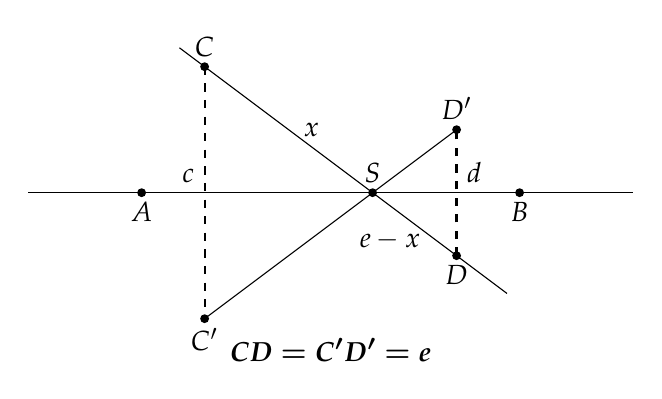
\begin{tikzpicture}[scale=.8]
\coordinate (A) at (-4,0);
\coordinate (B) at (2,0);
\coordinate (C) at (-3,2);
\coordinate (D) at (1,-1);
\coordinate (Cp) at (-3,-2);
\coordinate (Dp) at (1,1);
\fill (A) node[below] {$A$} circle[radius=2pt];
\fill (B) node[below] {$B$} circle[radius=2pt];
\fill (C) node[above] {$C$} circle[radius=2pt];
\fill (D) node[below] {$D$} circle[radius=2pt];
\fill (Cp) node[below] {$C'$} circle[radius=2pt];
\fill (Dp) node[above] {$D'$} circle[radius=2pt];
\draw[name path=ab] ($(A)!1.3!(B)$) -- ($(B)!1.3!(A)$);
\draw[name path=cd] ($(C)!1.2!(D)$) -- ($(D)!1.1!(C)$);
\path [name intersections={of=ab and cd,by={S}}];
\fill (S) node[above] {$S$} circle[radius=2pt];
\draw (Cp) -- (Dp);
\draw[thick,dashed] (C) -- node[above left] {$c$} (Cp);
\draw[thick,dashed] (D) -- node[above right] {$d$} (Dp);
\path (C) -- node[right,xshift=2pt] {$x$} (S);
\path (S) -- node[left,near end,xshift=-2pt] {$e-x$} (D);
\node at (-1,-2.5) {\mbox{\boldmath $CD=C'D'=e$}};
\end{tikzpicture}
\end{center}

Label $x=CS, c=CC', d=DD',e=CD$. $\triangle CSC'\sim\triangle DSD'$ are similar so $\disfrac{x}{e-x} = \frac{c}{d}$. Solving the equation for $x$ gives $x=\disfrac{c}{c+d}e$.

If $C,D$ are on the same side of $AB$:
\begin{center}
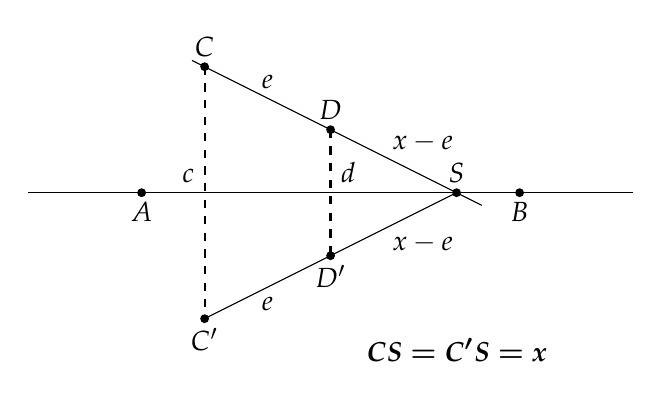
\begin{tikzpicture}[scale=.8]
\coordinate (A) at (-4,0);
\coordinate (B) at (2,0);
\coordinate (C) at (-3,2);
\coordinate (D) at (-1,1);
\coordinate (Cp) at (-3,-2);
\coordinate (Dp) at (-1,-1);
\fill (A) node[below] {$A$} circle[radius=2pt];
\fill (B) node[below] {$B$} circle[radius=2pt];
\fill (C) node[above] {$C$} circle[radius=2pt];
\fill (D) node[above] {$D$} circle[radius=2pt];
\fill (Cp) node[below] {$C'$} circle[radius=2pt];
\fill (Dp) node[below] {$D'$} circle[radius=2pt];
\draw[name path=ab] ($(A)!1.3!(B)$) -- ($(B)!1.3!(A)$);
\draw[name path=cd] ($(C)!2.2!(D)$) -- ($(D)!1.1!(C)$);
\path [name intersections={of=ab and cd,by={S}}];
\fill (S) node[above] {$S$} circle[radius=2pt];
\draw (Cp) -- (S);
\draw[thick,dashed] (C) -- node[above left] {$c$} (Cp);
\draw[thick,dashed] (D) -- node[above right] {$d$} (Dp);
\path (C) -- node[above] {$e$} (D);
\path (Cp) -- node[below] {$e$} (Dp);
\path (D) -- node[above right,xshift=-4pt] {$x-e$} (S);
\path (Dp) -- node[below right,xshift=-4pt] {$x-e$} (S);
\node at (1,-2.5) {\mbox{\boldmath $CS=C'S=x$}};
\end{tikzpicture}
\end{center}
$\triangle CSC'\sim\triangle DSD'$ gives $\disfrac{x}{x-e}=\disfrac{c}{d}$. Solving for $x$ gives $x=\disfrac{c}{c-d}e$.

Construct the circles $c(C',d), c(D,e)$ and label their intersection by $H$. The sum of the line segments $CC',C'H$ is $c + d$. We have to show that $H$ is on the extension of $CC'$ so that $CH$ is a line segment of length $c+d$. ($CH = c - d$ in case $D$ is on the same side of $AB$ as $C$.) 

\vspace{-3ex}

\begin{center}
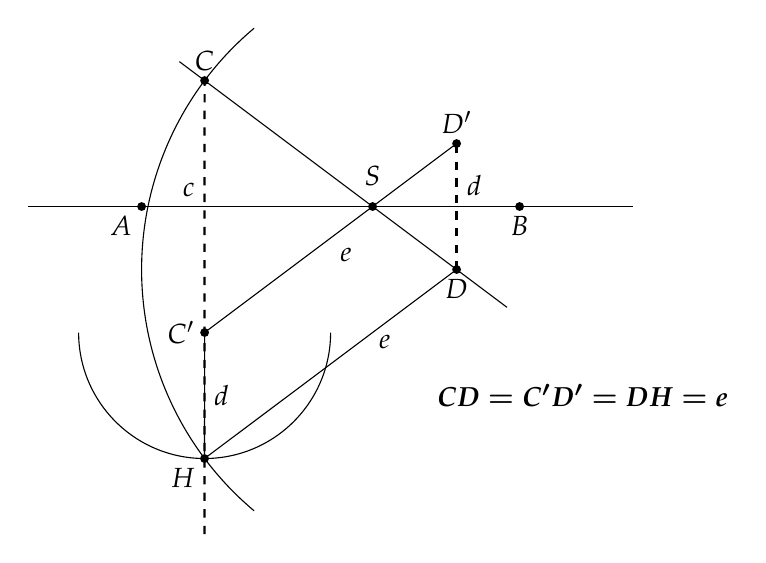
\begin{tikzpicture}[scale=.8]
\coordinate (A) at (-4,0);
\coordinate (B) at (2,0);
\coordinate (C) at (-3,2);
\coordinate (D) at (1,-1);
\coordinate (Cp) at (-3,-2);
\coordinate (Dp) at (1,1);
\fill (A) node[below left] {$A$} circle[radius=2pt];
\fill (B) node[below] {$B$} circle[radius=2pt];
\fill (C) node[above] {$C$} circle[radius=2pt];
\fill (D) node[below] {$D$} circle[radius=2pt];
\fill (Cp) node[left] {$C'$} circle[radius=2pt];
\fill (Dp) node[above] {$D'$} circle[radius=2pt];
\draw[name path=ab] ($(A)!1.3!(B)$) -- ($(B)!1.3!(A)$);
\draw[name path=cd] ($(C)!1.2!(D)$) -- ($(D)!1.1!(C)$);
\path [name intersections={of=ab and cd,by={S}}];
\fill (S) node[above,yshift=4pt] {$S$} circle[radius=2pt];
\draw (Cp) -- node[below right] {$e$} (Dp);
\path (C) -- node[above left] {$c$} (Cp);
\draw[thick,dashed] (D) -- node[above right] {$d$} (Dp);
\node at (3,-3) {\mbox{\boldmath $CD=C'D'=DH=e$}};
\draw[name path=circled] (D) let
  \p1 = ($ (D) - (C) $),
  \n2 = {veclen(\x1,\y1)}
in
  ++(130:\n2) arc (130:230:\n2);

\draw[name path=circlecp] (Cp) let
  \p1 = ($ (D) - (Dp) $),
  \n2 = {veclen(\x1,\y1)}
in
  ++(-180:\n2) arc (-180:0:\n2);
\path [name intersections={of=circled and circlecp,by={H}}];
\fill (H) node[below left] {$H$} circle[radius=2pt];
\draw[thick,dashed] ($(C)!1.2!(H)$) -- (C);
\draw (H) -- node[right] {$d$} (Cp);
\draw (D) -- node[right,xshift=14pt,yshift=8pt] {$e$} (H);
\end{tikzpicture}
\end{center}

\vspace{-3ex}

From the definition of $H$ as the intersection of $c(C',d)$,$c(D,e)$, we get $DH=e$, $C'H=d$, but $C'D' = e$, $D'D=d$, so the quadrilateral $C'D'DH$ is a parallelogram, since the lengths of both pairs of opposite sides are equal. By construction, the line segment $DD'$ is parallel to $CC'$, so $C'H$ is parallel to $DD'$ is also parallel to $CC'$. Since one of its end points is $C'$, it must be on the line containing $CC'$.

The lengths $c,d,e$ are given and we proved in Section~\ref{s.add-subtract} that a line segment of length $c+d$ can be construction and in Section~\ref{s.three} that a line segment of length $x=\disfrac{c}{c+d}e$ can be constructed. $S$ is the intersection of $c(C',x)$ and $c(C,x)$.

\begin{center}
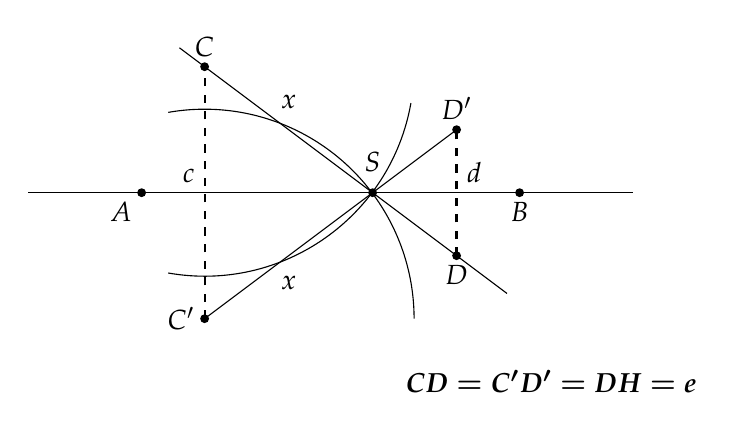
\begin{tikzpicture}[scale=.8]
\coordinate (A) at (-4,0);
\coordinate (B) at (2,0);
\coordinate (C) at (-3,2);
\coordinate (D) at (1,-1);
\coordinate (Cp) at (-3,-2);
\coordinate (Dp) at (1,1);
\fill (A) node[below left] {$A$} circle[radius=2pt];
\fill (B) node[below] {$B$} circle[radius=2pt];
\fill (C) node[above] {$C$} circle[radius=2pt];
\fill (D) node[below] {$D$} circle[radius=2pt];
\fill (Cp) node[left] {$C'$} circle[radius=2pt];
\fill (Dp) node[above] {$D'$} circle[radius=2pt];
\draw[name path=ab] ($(A)!1.3!(B)$) -- ($(B)!1.3!(A)$);
\draw[name path=cd] ($(C)!1.2!(D)$) -- ($(D)!1.1!(C)$);
\path [name intersections={of=ab and cd,by={S}}];
\fill (S) node[above,yshift=4pt] {$S$} circle[radius=2pt];
\draw (Cp) -- (Dp);
\path (C) -- node[above,yshift=4pt] {$x$} (S);
\path (Cp) -- node[below,yshift=-4pt] {$x$} (S);
\path (C) -- node[above left] {$c$} (Cp);
\draw[thick,dashed] (D) -- node[above right] {$d$} (Dp);
\node at (2.5,-3) {\mbox{\boldmath $CD=C'D'=DH=e$}};
\draw[name path=circled] (C) let
  \p1 = ($ (S) - (C) $),
  \n2 = {veclen(\x1,\y1)}
in
  ++(-10:\n2) arc (-10:-100:\n2);

\draw[name path=circlecp] (Cp) let
  \p1 = ($ (S) - (C) $),
  \n2 = {veclen(\x1,\y1)}
in
  ++(100:\n2) arc (100:0:\n2);
\draw[thick,dashed] (Cp) -- (C);
\end{tikzpicture}
\end{center}

%%%%%%%%%%%%%%%%%%%%%%%%%%%%%%%%%%%%%%%%%%%%%%%%%%%%%%%%%%%%%%%

\section{Finding the intersection of a line and a circle}\label{s.line-circle}

\textbf{Given a circle $k=C(M,r)$ and a line $AB$, it is possible to construct their intersections using only a compass.}

Construct $M'$, be the reflection of $M$ about $AB$ and the circle $k'=c(M',r)$. The points of intersection of $k,k'$ are the points of intersection of the line $AB$ and the circle $k$.

\begin{center}
\begin{tikzpicture}[scale=.5]
\coordinate (A) at (-7,0);
\coordinate (B) at (8,0);
\coordinate (M) at (0,-2);
\coordinate (Mp) at (0,2);
\fill (A) node[below] {$A$} circle[radius=3pt];
\fill (B) node[below] {$B$} circle[radius=3pt];
\fill (M) node[below left] {$M$} circle[radius=3pt];
\fill (Mp) node[above left] {$M'$} circle[radius=2pt];
\draw[name path=c1] (M) circle[radius=3cm];
\draw[name path=c2] (Mp) circle[radius=3cm];
\draw[name path=ab] ($(A)!1.2!(B)$) -- ($(B)!1.2!(A)$);
\path [name intersections={of=c1 and c2,by={S1,S2}}];
\fill (S1) circle[radius=3pt];
\fill (S2) circle[radius=3pt];
\path[name path=radius1] (M) -- ++(15:4cm);
\path [name intersections={of=c1 and radius1,by={R1}}];
\draw[thick,dashed] (M) -- node[below] {$r$} (R1);
\path[name path=radius2] (Mp) -- ++(40:4cm);
\path [name intersections={of=c2 and radius2,by={R2}}];
\draw[thick,dashed] (Mp) -- node[above] {$r$} (R2);
\fill (R1) circle[radius=3pt];
\fill (R2) circle[radius=3pt];
\end{tikzpicture}
\end{center}

This construction cannot be done if $M$ is on the line $AB$. In this case, extend and shorten $AM$ by length $r$ as described in Section~\ref{s.add-subtract}. The end points of the extended and shortened segments are the intersections of $k$ with $AB$.


\begin{center}
\begin{tikzpicture}[scale=.5]
\coordinate (A) at (-7,0);
\coordinate (B) at (8,0);
\coordinate (M) at (0,0);
\fill (A) node[below] {$A$} circle[radius=3pt];
\fill (B) node[below] {$B$} circle[radius=3pt];
\fill (M) node[below left] {$M$} circle[radius=3pt];
\draw[name path=c1] (M) circle[radius=3cm];
\draw[name path=ab] ($(A)!1.2!(B)$) -- ($(B)!1.2!(A)$);
\path[name path=radius1] (M) -- ++(-30:4cm);
\path [name intersections={of=c1 and radius1,by={R1}}];
\draw[thick,dashed] (M) -- node[below] {$r$} (R1);
\path [name intersections={of=c1 and ab,by={S1,S2}}];
\fill (S1) node[above right] {$AM+r$} circle[radius=3pt];
\fill (S2) node[above left] {$AM-r$} circle[radius=3pt];
\fill (R1) circle[radius=3pt];
\end{tikzpicture}
\end{center}



\tikzsetfigurename{straightedge-only}
% !TeX root = construct.tex

\selectlanguage{hebrew}

\chapter{אני מסתפק בסרגל )ועוד משהו(}

%%%%%%%%%%%%%%%%%%%%%%%%%%%%%%%%%%%%%%%%%%%%%%%%%%%%%%%%%%%%%%%


האם כל בנייה בסרגל ומחוגה ניתנת לבנייה עם סרגל בלבד? התשובה היא שלילית. ב-%
$1822$
המתיטיקאי הצרפתי
\L{Jean-Victor Poncelet}
שיער שכן ניתן להסתפק בסרגל בלבד, בתנאי שקיים במישור מעגל
\textbf{%
אחד%
}.
המשפט הוכח ב-
$1833$
על ידי המתימטיקאי השוויצרי
\L{Jakob Steiner}.
בפרק זה אביא את הוכחת המשפט המבוססת על ההוכחה שמופיעה כבעייה
$34$
ב-%
\L{\cite{dorrie1}},
ועובדה על ידי
\L{Michael Woltermann} \L{\cite{dorrie2}}.%
\footnote{%
ברצוני להודות לו על הרשות להתשמש בעבודתו.
}

%%%%%%%%%%%%%%%%%%%%%%%%%%%%%%%%%%%%%%%%%%%%%%%%%%%%%%%%%%%%%%%


במאה ה-
$19$
הוכח שאם נתחיל עם קטע קו שאורכו 
$1$
)המידות לא משנות, פשוט קובעים שאורך הקטע הוא אחד(, ניתן לבנות קטעי קו באורכים המתקבלים מהמספרים הרציונליים על ידי פעולות החשבון 
$+,-,\times,\div$
ועוד פעולת שורש ריבועי 
$\rule[-5pt]{0pt}{20pt}\sqrt{}$,
\textbf{%
ורק%
}
מספרים אלה. עם סרגל בלבד ניתן למצוא את נקודת החיתוך של שני קווים, פעולה לשמעשה פותרת משוואה מסדר ראשון, כלומר, אי אפשר לחשב שורש ריבועי. הבנייה של
\L{Poncelet-Steiner}
מראה שאם קיים מעגל אחד, ניתן להשתמש בו כדי לחשב שורש ריבועי וכך לבניות כל בנייה עםf סרגל ומחוגה.

%%%%%%%%%%%%%%%%%%%%%%%%%%%%%%%%%%%%%%%%%%%%%%%%%%%%%%%%%%%%%%%

כל צעד בבנייה על סרגל ומחוגה הוא אחת משלושת פעולות האלו:
\begin{itemize}
\setlength{\itemsep}{0pt}
\item
מציאת נקודת החיתוך של שני קווים ישרים.
\item
מציאת נקודות החיתוך של קו ישר עם מעגל.
\item
מציאת נקודות החיתוך של שני מעגלים.
\end{itemize}
ברור שניתן לבצע את הפעולה הראשונה עם סרגל בלבד. עלינו להראות שעבור שתי הפעולות הראשונות ניתן למוצא בנייה שקולה המשתמשת רק בסרגל עם מעגל אחד.

%%%%%%%%%%%%%%%%%%%%%%%%%%%%%%%%%%%%%%%%%%%%%%%%%%%%%%%%%%%%%%%

מה המשמעות של בנייה עם סרגל בלבד? מעגל מוגדר על ידי נקודה
$O$,
שהיא מרכז המעגל, וקטע קו באורך
$r$,
הרדיוס, שאחת מהנקודות הקצה שלה היא
$O$.
אם נצליח לבנות את הנקודות
$X,Y$
המסומנות בהתרשים שלהלן, נוכל לטעון שהצלחנו לבנות את נקודות החיתוך של מעגל נתון עם קו נתון ושל שני מעגלים. המעגלים המצויירים בקו מקווקוו לא ממש מפיעים בבנייה. בהמשך, המעגל היחיד הנתון יצוייר בקו רגיל, ומעגלים המשמשים רק להדגמת הבנייה והוכחתה יהיו מקווקווים.


\begin{center}
\selectlanguage{english}
\begin{tikzpicture}[scale=.9]
\fill (0,0) node[above right] {$O$} circle[radius=1.5pt];
\draw[thick,dashed,name path=circle] (0,0) circle[radius=2cm];
\draw (0,0) -- node[left] {$r$} ++(-60:2cm);
\fill (0,0) ++(-60:2cm) circle[radius=1.5pt];
\draw[name path=line] (-3,-.5) -- ++(20:6cm);
\path [name intersections={of=circle and line,by={X,Y}}];
\fill (X) node[above right,xshift=-2pt,yshift=4pt] {$X$} circle[radius=1.5pt];
\fill (Y) node[above left] {$Y$} circle[radius=1.5pt];
\begin{scope}[xshift=6cm]
\fill (0,0) node[above right] {$O_1$} circle[radius=1.5pt];
\fill (3,0) node[above right] {$O_2$} circle[radius=1.5pt];
\draw[thick,dashed,name path=circle1] (0,0) circle[radius=2cm];
\draw[thick,dashed,name path=circle2] (3,0) circle[radius=2cm];
\draw (0,0) -- node[left] {$r_1$} ++(-70:2cm);
\draw (3,0) -- node[left,below] {$r_2$} ++(-20:2cm);
\fill (0,0) ++(-70:2cm) circle[radius=1.5pt];
\fill (3,0) ++(-20:2cm) circle[radius=1.5pt];
\path [name intersections={of=circle1 and circle2,by={X,Y}}];
\fill (X) node[above,yshift=4pt] {$X$} circle[radius=1.5pt];
\fill (Y) node[below,yshift=-4pt] {$Y$} circle[radius=1.5pt];
\end{scope}
\end{tikzpicture}
\selectlanguage{hebrew}
\end{center}


%%%%%%%%%%%%%%%%%%%%%%%%%%%%%%%%%%%%%%%%%%%%%%%%%%%%%%%%%%%%%%%


תחילה נביא חמש בניות עזר נחוצות )סעיפים
\L{\ref{s.parallel}--\ref{s.root}}%
(,
ואחר כך נראה איך למצוא נקודות חיתוך של קו עם מעגל )סעיף
\L{\ref{s.line-circle-straight}}%
( ושל שני מעלגים )סעיף
\L{\ref{s.circle-circle}}%
(.

\np
%%%%%%%%%%%%%%%%%%%%%%%%%%%%%%%%%%%%%%%%%%%%%%%%%%%%%%%%%%%%%%%

\section{%
בניית קו המקביל לקו נתון%
}\label{s.parallel}

\textbf{%
נתון קו
$l$
המוגדר על ידי שתי נקודות
$A,B$,
ונקודה 
$P$
)שאיננה על הקו(, ניתן לבנות קו דרך
$P$
המקביל ל-%
$AB$.%
}

נפריד את הבנייה לשני מקרים:
\begin{itemize}
\item
"קו מכוון": נתונה הנקודה 
$M$
\textbf{%
החוצה
}
את
$AB$.
\item
כל קו אחר.
\end{itemize}

\vspace{-2ex}

\textbf{%
קו מכוון:
}
נבנה קרן הממשיכה את
$AP$,
ונבחר
$S$,
נקודה כלשהי על הקרן מעבר ל-%
$AP$.
נבנה את הקווים
$SB$, $SM$, $BP$.
נסמן ב-%
$O$
את נקודת החיתוך של 
$BP$
עם
$SM$.
נבנה קרן הממשיכה את
$AO$
ונסמן ב-%
$Q$
את החיתוך של הקרן
$AO$
עם
$SB$.
\begin{center}
\selectlanguage{english}
\vspace*{-4pt}
\begin{tikzpicture}
\draw[name path=pq] (-4,0) -- (4,0);
\draw (-2,-2) node[below left] {$A$} coordinate (A) -- (2,-2) node[below right] {$B$} coordinate (B);
\fill (A) circle[radius=1.5pt];
\fill (B) circle[radius=1.5pt];
\draw[name path=as] (A) -- ++(50:4cm) node[above] {$S$} coordinate (S);
\fill (S) circle[radius=1.5pt];
\draw[name path=sb] (S) -- (B);
\path [name intersections={of=pq and as,by={P}}];
\path [name intersections={of=pq and sb,by={Q}}];
\fill (P) node[above left] {$P$} circle[radius=1.5pt];
\fill (Q) node[above right] {$Q$} circle[radius=1.5pt];
\draw[name path=pb] (P) -- (B);
\draw[name path=qa] (Q) -- (A);
\path [name intersections={of=pb and qa,by={O}}];
\fill (O) node[right,xshift=2pt] {$O$} circle[radius=1.5pt];
\fill (0,-2) coordinate (M) node[below right] {$M$} circle[radius=1.5pt];
\draw (S) -- (M);
\end{tikzpicture}
\vspace*{-4pt}
\selectlanguage{hebrew}
\end{center}

\textbf{%
טענה:
$PQ$
מקביל ל-%
$AB$.}

\textbf{הוכחה:}
נשתמש במשפט של
\L{Ceva}
שנוכיח בהמשך.

\textbf{משפט:}
נתונים שלושה קווים מקודקודי משולש לצלעות הנגדיים שנפגשים בנקודה )כמו בתרשים, אבל 
$M$
לא בהכרח חוצה הצלע(, קטעי הצלעות מקיימים את היחס:
\[
\frac{AM}{MB}\cdot\frac{BQ}{QS}\cdot\frac{SP}{PA} = 1\,.
\]
$M$
חוצה את
$AB$
ולכן
$\disfrac{AM}{MB}=1$.
הגורם הראשון של המכלפה מצטמצם ונקבל את המשוואה:
\selectlanguage{english}
\begin{equation}
\frac{BQ}{QS}=\frac{PA}{SP}=\frac{AP}{PS}\,.\label{eq.ceva}
\end{equation}
\selectlanguage{hebrew}

\vspace{-3ex}

נוכיח שהמשולש
$\triangle ABS$
דומה ל-%
$\triangle PQS$,
ולכן הקו
$PQ$
מקביל לקו
$AB$
כי
$\angle ABS = \angle PQS$.
ההוכחה שהמשולשים דומים היא:
\vspace*{-10pt}
\erh{12pt}
\selectlanguage{english}
\begin{equationarray*}{rcl}
BS&=&BQ+QS\\
\disfrac{BS}{QS}&=&\disfrac{BQ}{QS}+\disfrac{QS}{QS} = \disfrac{BQ}{QS}+1\\
AS&=&AP+PS\\
\disfrac{AS}{PS} &=& \disfrac{AP}{PS} + \disfrac{PS}{PS} = \disfrac{AP}{PS} + 1\\
\end{equationarray*}
\erh{12pt}
\selectlanguage{english}
\begin{equationarray*}{rcl}
\disfrac{BS}{QS}=\disfrac{BQ}{QS}+1&=&\disfrac{AP}{PS} + 1=\disfrac{AS}{PS}\,,
\end{equationarray*}
\selectlanguage{hebrew}
כאשר המשוואה האחרונה מתקבלת מ-%
\L{\ref{eq.ceva}}.


\textbf{הוכחה של משפט \L{Ceva}:}
נתבונן בתרשימים שלהן:
\begin{center}
\selectlanguage{english}
\vspace*{-4pt}
\begin{tikzpicture}
\path[name path=pq] (-4,0) -- (4,0);
\draw (-2,-2) node[below left] {$A$} coordinate (A) -- (2,-2) node[below right] {$B$} coordinate (B);
\coordinate (M) at (0,-2);
\draw[name path=as] (A) -- ++(50:4cm) node[above] {$S$} coordinate (S);
\draw[name path=sb] (S) -- (B);
\path [name intersections={of=pq and as,by={P}}];
\path [name intersections={of=pq and sb,by={Q}}];
\path[name path=pb] (P) -- (B);
\path[name path=qa] (Q) -- (A);
\path [name intersections={of=pb and qa,by={O}}];
\draw[fill=gray!40] (B) -- (O) -- (Q);
\draw[fill=gray!70] (S) -- (O) -- (Q);
\draw (B) -- (O) -- (A);
\draw (S) -- (O) -- (A);
\draw (A) -- (B) -- (S) -- cycle;
\draw (S) -- (O);
\draw (B) -- (O);
\fill (A) circle[radius=1.5pt];
\fill (B) circle[radius=1.5pt];
\fill (S) circle[radius=1.5pt];
\fill (Q) node[above right] {$Q$} circle[radius=1.5pt];
\fill (O) node[above left] {$O$} circle[radius=1.5pt];
\path[name path=al1] (O) -- ($(Q)!(O)!(B)$);
\draw[rotate=-155] ($(Q)!(O)!(B)$) rectangle +(7pt,7pt);
\path [name intersections={of=al1 and sb,by={A1}}];
\draw[thick,dashed] (O) -- (A1);
\begin{scope}[xshift=6cm]
\path[name path=pq] (-4,0) -- (4,0);
\draw (-2,-2) node[below left] {$A$} coordinate (A) -- (2,-2) node[below right] {$B$} coordinate (B);
\coordinate (M) at (0,-2);
\draw[name path=as] (A) -- ++(50:4cm) node[above] {$S$} coordinate (S);
\draw[name path=sb] (S) -- (B);
\path [name intersections={of=pq and as,by={P}}];
\path [name intersections={of=pq and sb,by={Q}}];
\draw[name path=pb] (P) -- (B);
\draw[name path=qa] (Q) -- (A);
\path [name intersections={of=pb and qa,by={O}}];
\draw (B) -- (O) -- (Q);
\draw (A) -- (Q) -- (B);
\draw[fill=gray!40] (B) -- (Q) -- (A);
\draw[fill=gray!70] (S) -- (Q) -- (A);
\draw (A) -- (B) -- (S) -- cycle;
\draw (S) -- (O);
\draw (B) -- (O);
\fill (A) circle[radius=1.5pt];
\fill (B) circle[radius=1.5pt];
\fill (S) circle[radius=1.5pt];
\fill (Q) node[above right] {$Q$} circle[radius=1.5pt];
\fill (O) node[above left] {$O$} circle[radius=1.5pt];
\path[name path=al2] (A) -- ($(Q)!(A)!(B)$);
\draw[rotate=-155] ($(Q)!(A)!(B)$) rectangle +(7pt,7pt);
\path [name intersections={of=al2 and sb,by={A2}}];
\draw[thick,dashed] (A) -- (A2);
\end{scope}
\end{tikzpicture}
\vspace*{-6pt}
\selectlanguage{hebrew}
\end{center}
אם הגבהים של שני משולשים שוואים, יחס השטחים שווה ליחס הבסיסים.
%\[
%A_1 = \frac{1}{2}hb_1,\quad A_2 = \frac{1}{2}hb_2, \quad \frac{A_1}{A_2}=\frac{b_1}{b_2}\,.
%\]
בכל אחד מהתרשימים, הגבהים של זוג המשולשים המסומנים באפור שווים. לכן:%
\footnote{%
נשתמש בשם המשולש כקיצור לשטחו.%
}
\[\frac{\triangle BQO}{\triangle SQO} = \frac{BQ}{QS}\;,\quad\quad \frac{\triangle BQA}{\triangle SQA} = \frac{BQ}{QS}\;.
\]
על ידי חיסור של המשולשים המסומנים, נקבל יחס בין המשולשים המסומנים באפור:
\begin{center}
\selectlanguage{english}
\vspace*{-4pt}
\begin{tikzpicture}
\path[name path=pq] (-4,0) -- (4,0);
\draw (-2,-2) node[below left] {$A$} coordinate (A) -- (2,-2) node[below right] {$B$} coordinate (B);
\coordinate (M) at (0,-2);
\draw[name path=as] (A) -- ++(50:4cm) node[above] {$S$} coordinate (S);
\draw[name path=sb] (S) -- (B);
\path [name intersections={of=pq and as,by={P}}];
\path [name intersections={of=pq and sb,by={Q}}];
\path[name path=pb] (P) -- (B);
\draw[thick,name path=qa] (Q) -- (A);
\path [name intersections={of=pb and qa,by={O}}];
\draw[fill=gray!50] (B) -- (O) -- (A);
\draw[fill=gray!70] (S) -- (O) -- (A);
\draw (B) -- (O) -- (A);
\draw (S) -- (O) -- (A);
\draw (A) -- (B) -- (S) -- cycle;
\draw (S) -- (O);
\draw (B) -- (O);
\fill (A) circle[radius=1.5pt];
\fill (B) circle[radius=1.5pt];
\fill (S) circle[radius=1.5pt];
\fill (Q) node[above right] {$Q$} circle[radius=1.5pt];
\fill (O) node[right,xshift=2pt] {$O$} circle[radius=1.5pt];
\end{tikzpicture}
\vspace*{-4pt}
\selectlanguage{hebrew}
\end{center}
\[
\frac{BQ}{QS} = \frac{\triangle BQA - \triangle BQO}{\triangle SQA-\triangle SQO} = \frac{\triangle BOA}{\triangle SOA}\,.
\]
החישוב עלול להיראות חשוד. נסביר אותו תוך שימוש בסימונים פשוטים יותר:
\erh{10pt}
\begin{equationarray*}{rcl}
 \disfrac{c}{d} &=&\disfrac{a}{b}\\
 \disfrac{e}{f} &=&\disfrac{a}{b}\\
c-e &=& \disfrac{ad}{b} - \disfrac{af}{b}= \disfrac{a}{b}(d-f)\\
\disfrac{c-e}{d-f} &=& \disfrac{a}{b}\,.
\end{equationarray*}

\np

באופן דומה ניתן להוכיח:
\[
\frac{AM}{MB} = \frac{\triangle AOS}{\triangle BOS}\;,\quad\quad \frac{SP}{PA} =\frac{\triangle SOB}{\triangle AOB}\;,
\]
ומכאן:
\[
\frac{AM}{MB}\cdot\frac{BQ}{QS}\cdot\frac{SP}{PA} = \frac{\triangle AOS}{\triangle BOS}\frac{\triangle BOA}{\triangle SOA}\frac{\triangle SOB}{\triangle AOB}=1\,,
\]
כי
$\triangle AOS=\triangle SOA$, $\triangle BOA=\triangle AOB$, $\triangle SOB=\triangle BOS$.

\textbf{סוף הוכחה של משפט \L{Ceva}}.
%%%%%%%%%%%%%%%%%%%%%%%%%%%%%%%%%%%%%%%%%%%%%%%%%%%%%%%%%%%%%%%

\medskip

\textbf{%
כל קו אחר:
}

נסמן את הקו ב-%
$l$,
נסמן ב-%
$c$
את
\textbf{%
המעגל הקבוע%
}
שמרכזו בנקודה
$O$
והרדיוס שלו הוא
$r$,
ונסמן ב-%
$P$
את הנקודה שלא נמצאת על הקו שיש לבנות דרכו קו המקביל ל-%
$l$.
עליך להשתכנע שהבנייה לא תלוייה במיקום המעגל במישור או ברדיוס שלו.

נבחר 
$M$,
נקודה כלשהי על הקו 
$l$,
ונבנה קרן הממשיכה את
$MO$
והחותך את המעגל ב-%
$U,V$.
\begin{center}
\selectlanguage{english}
\begin{tikzpicture}[scale=.8]
\coordinate (O) at (0,0);
\fill (O) node[below right] {$O$} circle[radius=1.5pt];
\draw[name path=circle] (O) circle[radius=2cm];
\draw[name path=l] (-4,-3) -- node[above, near end] {$l$} +(9,0);
\path[name path=mo] (-2,-3) coordinate (M) -- ($(-2,-3)!1.65!(O)$);
\fill (M) node[below] {$M$} circle[radius=1.5pt];
\path [name intersections={of=circle and mo,by={V,U}}];
\fill (U) node[below,xshift=2pt,yshift=-4pt] {$U$} circle[radius=1.5pt];
\fill (V) node[right,xshift=4pt] {$V$} circle[radius=1.5pt];
\draw (M) -- (V);
\node at (-1.6,1.6) {$c$};
\fill (-4,1) node[above left] {$P$} circle[radius=1.5pt];
\end{tikzpicture}
\vspace*{-8pt}
\selectlanguage{hebrew}
\end{center}
קו זה הוא
\textbf{%
קו מכוון%
}
כי 
$O$,
מרכז המעגל, חוצה את הקוטר
$UV$.
נבחר נקודה שנייה 
$A$
על 
$l$
ונשתמש בבבנייה עבור קו מכוון כדי לבנות קו המקביל ל-%
$UV$.
הקו חותך את המעגל
$X,Y$.
\begin{center}
\selectlanguage{english}
\begin{tikzpicture}[scale=.9]
\coordinate (O) at (0,0);
\fill (O) node[below right] {$O$} circle[radius=1.5pt];
\draw[name path=circle] (O) circle[radius=2cm];
\draw[name path=l] (-4,-3) -- node[above,near end,xshift=24pt] {$l$} +(9,0);
\path[name path=mo] (-2,-3) coordinate (M) -- ($(-2,-3)!1.65!(O)$);
\fill (M) node[below] {$M$} circle[radius=1.5pt];
\path [name intersections={of=circle and mo,by={V,U}}];
\fill (U) node[below,xshift=2pt,yshift=-4pt] {$U$} circle[radius=1.5pt];
\fill (V) node[right,xshift=4pt] {$V$} circle[radius=1.5pt];
\draw (M) -- (V);
\path[name path=ax] (-3,-3) coordinate (A) -- ($(-3,-3)!1.8!(-1,0)$);
\fill (A) node[below] {$A$} circle[radius=1.5pt];
\path [name intersections={of=circle and ax,by={Y,X}}];
\fill (X) node[left] {$X$} circle[radius=1.5pt];
\fill (Y) node[above] {$Y$} circle[radius=1.5pt];
\node at (-1.6,1.6) {$c$};
\draw (A) -- (Y);
\fill (-4,1) node[above left] {$P$} circle[radius=1.5pt];
\end{tikzpicture}
\vspace*{-6pt}
\selectlanguage{hebrew}
\end{center}
נבנה קוטר
$XX'$
וקוטר
$YY'$.
נבנה קרן מ-%
$X'Y'$
ונסמן ב-%
$B$
את נקודת החיתוך שלה עם 
$l$.

\np

\begin{center}
\selectlanguage{english}
\begin{tikzpicture}[scale=.9]
\coordinate (O) at (0,0);
\fill (O) node[below right] {$O$} circle[radius=1.5pt];
\draw[name path=circle] (O) circle[radius=2cm];
\draw[name path=l] (-4,-3) -- node[above,near end,xshift=24pt] {$l$} +(9,0);
\path[name path=mo] (-2,-3) coordinate (M) -- ($(-2,-3)!1.65!(O)$);
\fill (M) node[below] {$M$} circle[radius=1.5pt];
\path [name intersections={of=circle and mo,by={V,U}}];
\fill (U) node[below,xshift=2pt,yshift=-4pt] {$U$} circle[radius=1.5pt];
\fill (V) node[right,xshift=4pt] {$V$} circle[radius=1.5pt];
\draw (M) -- (V);
\path[name path=ax] (-3,-3) coordinate (A) -- ($(-3,-3)!1.8!(-1,0)$);
\fill (A) node[below] {$A$} circle[radius=1.5pt];
\path [name intersections={of=circle and ax,by={Y,X}}];
\fill (X) node[left] {$X$} circle[radius=1.5pt];
\fill (Y) node[above] {$Y$} circle[radius=1.5pt];
\node at (-1.6,1.6) {$c$};
\draw (A) -- (Y);
\fill (-4,1) node[above left] {$P$} circle[radius=1.5pt];
\path[name path=xo] (X) -- ($(X)!2.2!(O)$);
\path[name intersections={of=circle and xo,by={Xp}}];
\fill (Xp) node[right,xshift=2pt,yshift=-2pt] {$X'$} circle[radius=1.5pt];
\draw (X) -- (Xp);
\path[name path=yo] (Y) -- ($(Y)!2.4!(O)$);
\path[name intersections={of=circle and yo,by={Yp,y}}];
\fill (Yp) node[below right] {$Y'$} circle[radius=1.5pt];
\draw (Y) -- (Yp);
\path[name path=xy] (Xp) -- ($(Xp)!1.6!(Yp)$);
\path[name intersections={of=l and xy,by={B}}];
\fill (B) node[below] {$B$} circle[radius=1.5pt];
\draw (Xp) -- (B);
\draw[thick,dashed,name path=z] (-4,0) -- (4,0) node[above,near end,xshift=40pt] {$l'$};
\path[name intersections={of=ax and z,by={Z}}];
\path[name intersections={of=xy and z,by={Zp}}];
\fill (Z) node[above left] {$Z$} circle[radius=1.5pt];
\fill (Zp) node[below right] {$Z'$} circle[radius=1.5pt];
\end{tikzpicture}
\vspace*{-10pt}
\selectlanguage{hebrew}
\end{center}
\textbf{%
טענה:%
}
$l$
הוא
\textbf{%
קו מכוון%
}
כי
$M$
חוצה את
$AB$.

מהטענה אפשר לבנות קו דרך 
$P$
מקביל ל-%
$AB$
לפי הבנייה עבור קו מכוון.

\textbf{%
הוכחה:%
}
$OX,OX',OY,OY'$
הם כולם רדיוסים של המעגל, ו-%
$\angle XOY = \angle X'OY'$
כי הן זוויות נגדיות. לכן,
$\triangle XOY\cong \triangle X'OY'$
לפי צ.ז.צ. נגדיר )לא נבנה!(
$l'$,
קו מקביל ל-%
$l$,
החותך את 
$XY$
ב-%
$Z$
והחותך את 
$X',Y'$
ב-%
$Z'$.
$\angle XOZ=\angle X'OZ'$
כי הן זוויות נגדיות, ולכן
$\triangle XOZ\cong \triangle X'OZ'$
לפי ז.צ.ז. ו-%
$ZO=OZ'$. 
$AMOZ$
ו-%
$BMOZ'$
מקביליות )מרובעים עם צלעות נגדיות מקבילות(, ולכן
$AM=ZO=OZ'=MB$.

\textbf{%
מסקנה:%
}
נתון קטע קו 
$AB$
ונקודה
$P$
שאיננה על הקו. ניתן לבנות קטע קו
$PQ$
המקביל ל-%
$AB$,
שאורכו שווה לאורכו של
$AB$.
במילים אחרות: ניתן להעתיק את
$AB$
מקביל לעצמו כך שקצה אחד יהיה נקודה כלשהי
$P$.

\textbf{%
הוכחה:%
}
בסעיף זה הוכחנו שניתן לבנות קו 
$m$
דרך 
$P$
המקביל ל-%
$AB$,
וקו
$n$
דרך 
$B$
המקביל ל-%
$AP$.
המרובע 
$ABQP$
הוא מקבילית, ולכן הצלעות הנגדיות שוות:
$AB=PQ$.
\begin{center}
\selectlanguage{english}
\begin{tikzpicture}[scale=.7]
\coordinate (A) at (0,0);
\coordinate (B) at (3,0);
\coordinate (P) at (-2,2.5);
\coordinate (Q) at (1,2.5);
\draw ($(P)!-.6!(Q)$) -- node[above,near end,xshift=36pt] {$m$} ($(P)!1.8!(Q)$);
\fill (P) node[above] {$P$} circle[radius=1.5pt];
\fill (Q) node[above right] {$Q$} circle[radius=1.5pt];
\draw ($(A)!-.6!(B)$) -- node[above,near end,xshift=40pt] {$l$} ($(A)!2.5!(B)$);
\fill (A) node[below] {$A$} circle[radius=1.5pt];
\fill (B) node[below left] {$B$} circle[radius=1.5pt];
\draw (A) -- (P);
\draw ($(B)!-.3!(Q)$) -- node[above,near end,xshift=24pt,yshift=-24pt] {$n$} ($(B)!1.4!(Q)$);
\end{tikzpicture}
\selectlanguage{hebrew}
\end{center}

%%%%%%%%%%%%%%%%%%%%%%%%%%%%%%%%%%%%%%%%%%%%%%%%%%%%%%%%%%%%%%%

\section{%
בניית אנך לקו נתון%
}\label{s.perpendicular}

\textbf{%
נתון קו
$l$
ונקודה
$P$
)שאיננה על הקו( ניתן לבנות אנך ל-%
$l$
דרך
$P$.%
}

נבנה )לפי סעיף
\L{\ref{s.parallel}}(
קו
$l'$
מקביל ל-%
$l$
החותך את
\textbf{%
המעגל הקבוע%
}
ב-%
$U,V$.
נבנה את הקוטר
$UOU'$
והמיתר
$U'V$.

\np

\begin{center}
\selectlanguage{english}
\begin{tikzpicture}[scale=.8]
\coordinate (O) at (0,0);
\coordinate (P) at (3.5,.6);
\node at (-1.6,1.6) {$c$};
\draw[name path=circle] (O) circle[radius=2cm];
\draw[name path=l] (-4,-3) -- node[above,near end,xshift=45pt] {$l$} ++(9.5,0);
\draw[name path=lp] (-3,-1) -- node[above,near end,xshift=45pt] {$l'$} ++(7.5,0);
\fill (O) node[above left] {$O$} circle[radius=1.5pt];
\fill (P) node[right] {$P$} circle[radius=1.5pt];
\path[name intersections={of=circle and lp,by={U,V}}];
\fill (U) node[below left] {$U$} circle[radius=1.5pt];
\fill (V) node[below right] {$V$} circle[radius=1.5pt];
\path[name path=d] (U) -- ($(U)!2.3!(O)$);
\path[name intersections={of=circle and d,by={Up}}];
\draw (U) -- (Up);
\fill (Up) node[above right] {$U'$} circle[radius=1.5pt];
\draw (Up) -- (V);
\path[name path=p] (P) -- ++(0,-4);
\draw[name intersections={of=p and l,by={X}}];
\fill (X) circle[radius=1.5pt];
\draw[thick,dashed] (P) -- (X);
\draw ($(U)!.9!(V)$) -- ++(0,.3) -| (V);
\end{tikzpicture}
\vspace*{-8pt}
\selectlanguage{hebrew}
\end{center}
$\angle UVU'$
היא זווית ישרה כי היא נשענת על מחצית המעגל. מכאן ש-%
$U'V$
הוא אנך ל-%
$UV$
ו-%
$l'$.
נבנה קו מקביל ל-%
$U'V$
 דרך 
$P$
)לפי סעיף
\L{\ref{s.parallel}}(.



%%%%%%%%%%%%%%%%%%%%%%%%%%%%%%%%%%%%%%%%%%%%%%%%%%%%%%%%%%%%%%%

\section{%
העתקת קטע קו נתון בכיוון נתון%
}\label{s.direction}

\textbf{%
נתון נקודה
$A$,
קטע קו
$PQ$
וכיוון, ניתן לבנות קטע קו
$AS$
כך ש-%
$AS=PQ$.%
}

המסקנה בסוף סעיף
\L{\ref{s.parallel}}
מראה שאפשר להעתיק קטע קו מקביל לעצמו. כאן נוכיח שניתן להנתיק קטע קו בכיוון של כל קו אחר. הכוונה של "כיוון" היא שקו המוגדר על ידי שתי נקודות
$A',H'$
מגדיר זווית
$\theta$
יחסית לציר כלשהו. המשימה היא להעתיק את קטע הקו
$PQ$
ל-%
$AS$,
כך ש-%
$AS$
יהיה באותה זווית
$\theta$
יחסית לאותו ציר. בתרשים
$PQ$
נמצא על ציר ה-%
$x$
אבל אין לזה חשיבות.
\begin{center}
\selectlanguage{english}
\vspace*{-8pt}
\begin{tikzpicture}[scale=.8]
\coordinate (A) at (0,0);
\coordinate (P) at (1,-1.5);
\coordinate (Q) at (2.5,-1.5);
\draw (P) -- (Q);
\fill (P) node[left] {$P$} circle[radius=1.5pt];
\fill (Q) node[right] {$Q$} circle[radius=1.5pt];
\coordinate (A1) at (-4,1);
\draw[thick,dashed] (A1) -- ++(60:3cm) coordinate (H1);
\draw[thick,dashed] (A1) -- ++(0:3cm);
\fill (A1) node[left] {$A'$} circle[radius=1.5pt];
\fill (H1) node[left] {$H'$} circle[radius=1.5pt];
\draw (A) -- ++(60:1.5cm) coordinate (S);
\fill (S) node[above right] {$S$} circle[radius=1.5pt];
\draw[thick,dashed] (A) -- ++(3,0);
\fill (A) node[left] {$A$} circle[radius=1.5pt];
\node[above right,xshift=4pt] at (A1) {$\theta$};
\node[above right,xshift=4pt] at (A) {$\theta$};
\end{tikzpicture}
%\vspace*{-12pt}
\selectlanguage{hebrew}
\end{center}
לפי
\L{\ref{s.parallel}}
ניתן לבנות קטע הקו
$AH$
כך ש-%
$AH\|A'H'$,
וגם לבנות קטע קו
$AK$
כך ש-%
$AK\|PQ$.
\begin{center}
\selectlanguage{english}
\vspace*{-4pt}
\begin{tikzpicture}[scale=.8]
\coordinate (A) at (0,0);
\coordinate (P) at (1,-1.5);
\coordinate (Q) at (2.5,-1.5);
\draw (P) -- (Q);
\fill (P) node[left] {$P$} circle[radius=1.5pt];
\fill (Q) node[right] {$Q$} circle[radius=1.5pt];
\coordinate (A1) at (-3,1);
\draw (A1) -- ++(60:3cm) coordinate (H1);
\draw[thick,dashed] (A1) -- ++(0:1.5cm);
\fill (A1) node[left] {$A'$} circle[radius=1.5pt];
\fill (H1) node[left] {$H'$} circle[radius=1.5pt];
\draw (A) -- ++(60:3cm) coordinate (H);
\fill (H) node[left] {$H$} circle[radius=1.5pt];
\draw (A) -- ++(1.5,0) coordinate (K);
\fill (K) node[below right] {$K$} circle[radius=1.5pt];
\draw (A) -- (K);
\fill (A) node[left] {$A$} circle[radius=1.5pt];
\node[above right,xshift=4pt] at (A1) {$\theta$};
\node[above right,xshift=4pt] at (A) {$\theta$};
\end{tikzpicture}
\vspace*{-8pt}
\selectlanguage{hebrew}
\end{center}
הזווית
$\angle HAK$
שווה ל-%
$\theta$,
לכן כל מה שנשאר הוא למצוא נקודה
$S$
על
$AH$
כך ש-%
$AS=AK$.

\np

\textbf{%
במעגל הקבוע%
}
$c$
נבנה שני רדיוסים
$OU$
ו-%
$OV$
מקביליים ל-%
$AH$
ו-%
$AK$,
בהתאמה, ונבנה קרן דרך
$K$
המקבילה ל-%
$UV$.
נסמן את נקודת החיתוך של הקו עם
$AH$
ב-%
$S$.

\textbf{%
טענה:
}
$AS=PQ$.
\begin{center}
\selectlanguage{english}
\begin{tikzpicture}[scale=.8]
\coordinate (A) at (0,0);
\coordinate (P) at (1,-1.5);
\coordinate (Q) at (2.5,-1.5);
\draw (P) -- (Q);
\fill (P) node[left] {$P$} circle[radius=1.5pt];
\fill (Q) node[right] {$Q$} circle[radius=1.5pt];
\coordinate (A1) at (-3,1);
\draw (A1) -- ++(60:3cm) coordinate (H1);
\fill (A1) node[left] {$A'$} circle[radius=1.5pt];
\fill (H1) node[left] {$H'$} circle[radius=1.5pt];
\draw (A) -- ++(60:3cm) coordinate (H);
\fill (A) node[left] {$A$} circle[radius=1.5pt];
\fill (H) node[left] {$H$} circle[radius=1.5pt];
\coordinate (O) at (6,1);
\node at (4.8,3.4) {$c$};
\draw[name path=circle] (O) circle[radius=2.5cm];
\fill (O) node[above left] {$O$} circle[radius=1.5pt];
\draw (A) -- ++(1.5,0) coordinate (K);
\fill (K) node[below right] {$K$} circle[radius=1.5pt];
\draw (A) -- (K);
\path[name path=u] (O) -- ++(60:2.5cm);
\path[name path=v] (O) -- ++(2.5,0);
\path[name intersections={of=circle and u,by={U}}];
\path[name intersections={of=circle and v,by={V}}];
\fill (U) node[above right] {$U$} circle[radius=1.5pt];
\fill (V) node[right] {$V$} circle[radius=1.5pt];
\draw (O) -- (U) -- (V) -- cycle;
\path (A) -- ++(60:1.5cm) coordinate (S);
\fill (S) node[right] {$S$} circle[radius=1.5pt];
\draw (K) -- ($(K)!1.8!(S)$);
\draw (A) -- (S);
\node[above right,xshift=4pt] at (A) {$\theta$};
\node[above right,xshift=4pt] at (O) {$\theta$};
\node[above right,xshift=4pt] at (A1) {$\theta$};
\draw[thick,dashed] (A1) -- ++(1.5,0);
\end{tikzpicture}
%\vspace*{-4pt}
\selectlanguage{hebrew}
\end{center}
\textbf{%
הוכחה:
}
לפי הבנייה,
$AH\|OU$
ו-%
$AK\|OV$,
ולכן
$\angle SAK=\theta=\angle UOV$.
$SK\|UV$,
ו-%
$\triangle SAK\sim \triangle UOV$
לפי ז.ז.ז.
$\triangle UOV$
הוא משולש שווה שוקיים כי
$OU$, $OV$
הם רדיוסים של אותו מעגל. מכאן,
$\triangle SAK$
הוא משולש שווה שוקיים ו-%
$AS=AK=PQ$.



%%%%%%%%%%%%%%%%%%%%%%%%%%%%%%%%%%%%%%%%%%%%%%%%%%%%%%%%%%%%%%%

\section{%
בניית קטע קו שאורכו מוגדר יחסית לשלושה קטעי קו אחרים%
}\label{s.relative-straight}

\textbf{%
נתון קטעי קו באורכים
$n, m, s$,
ניתן לבנות קטע קו באורך
$x=\disfrac{n}{m}s$.%
}

קטעי הקו הנתונים נמצאים במיקומים כלשהם במישור ובכיוונים כלשהם.
\begin{center}
\selectlanguage{english}
\begin{tikzpicture}[scale=.9]
\draw (0,0) -- node[above] {$s$} ++(30:1.5cm);
\draw (2,1.2) -- node[above] {$m$} ++(-10:2.5cm);
\draw (-2,1.5) -- node[above] {$n$} ++(5:2cm);
\fill (0,0) circle[radius=1.5pt];
\fill (2,1.2) circle[radius=1.5pt];
\fill (-2,1.5) circle[radius=1.5pt];
\fill (0,0) ++(30:1.5cm) circle[radius=1.5pt];
\fill (2,1.2) ++(-10:2.5cm) circle[radius=1.5pt];
\fill (-2,1.5) ++(5:2cm) circle[radius=1.5pt];
\end{tikzpicture}
\vspace*{-8pt}
\selectlanguage{hebrew}
\end{center}
נבחר נקודה כלשהי
$A$
ונבנה שתי קרנות 
$AB,AC$.
לפי
\L{\ref{s.direction}}
ניתן לבנות נקודות
$M,N,S$
כך ש-%
$AM= m$, $AN =n$
ו-%
$AS=s$.
נבנה דרך
$N$
קו המקביל ל-%
$MS$
החותך את
$AC$
ב-%
$X$,
ונסמן את אורכו ב-%
$x$.
$\triangle MAS\sim \triangle NAX$
לפי ז.ז.ז., ולכן:
\[
\frac{m}{n}=\frac{s}{x}, \quad\quad x=\disfrac{n}{m}s\,.
\]
\begin{center}
\selectlanguage{english}
\vspace*{-10pt}
\begin{tikzpicture}
\coordinate (A) at (0,0);
\draw[name path=ac] (A) node[left] {$A$} -- ++(7,0) node[right] {$C$};
\draw (A) -- ++(40:5cm) node[right] {$B$};
\fill (A) circle[radius=1.5pt];
\fill (A) ++(40:5cm) circle[radius=1.5pt];
\fill (A) ++(7,0) circle[radius=1.5pt];
\path (A) -- node[above,xshift=-2pt] {$m$} ++(40:3cm) coordinate (M) node[above left] {$M$};
\path (A) -- ++(40:4cm) coordinate (N) node[above left] {$N$};
\fill (M) circle[radius=1.5pt];
\fill (N) circle[radius=1.5pt];
\path[name path=ms] (M) -- ++(-50:3.5cm);
\path[name path=nx] (N) -- ++(-50:4cm);
\path[name intersections={of=ac and ms,by={S}}];
\path[name intersections={of=ac and nx,by={X}}];
\fill (S) circle[radius=1.5pt] node[below] {$S$};
\fill (X) circle[radius=1.5pt] node[below] {$X$};
\path (A) -- node[below] {$s$} (S);
\draw (S) -- (M);
\draw (X) -- (N);
\node at (7,2.5) {$AN=n$};
\node at (7,2) {$AX=x$};
\end{tikzpicture}
\selectlanguage{hebrew}
\end{center}

\np

%%%%%%%%%%%%%%%%%%%%%%%%%%%%%%%%%%%%%%%%%%%%%%%%%%%%%%%%%%%%%%%

\section{%
בניית שורש ריבועי%
}\label{s.root}

\textbf{%
נתון קטעי קו באורכים
$a,b$,
ניתן לבעות קטע קו שאורכו
$\rule[-5pt]{0pt}{10pt}\sqrt{ab}$.}

אנו שואפים לבטא את
$\rule[-5pt]{0pt}{20pt}x=\sqrt{ab}$
בצורה
$x=\disfrac{n}{m}s$
כדי להשתמש בבנייה מ-%
\L{\ref{s.relative-straight}}.
\vspace*{-1ex}
\begin{itemize}
\setlength{\itemsep}{0pt}
\item עבור
$n$
נשתמש ב-%
$d$,
הקוטר של
\textbf{%
המעגל הקבוע%
}.
\item עבור
$m$
נשתמש ב-%
$t=a+b$
שניתן לבנות מהאורכים הנתונים
$a,b$
לפי
\L{\ref{s.direction}}.
\item 
נגדיר
$s=\sqrt{hk}$
כאשר 
$h,k$
מוגדרים כביטויים מעל האורכים
$a,b,t,d$,
ונראה איך ניתן לבנות קטע קו באורך 
$\sqrt{hk}$.
\end{itemize}
\vspace{-1ex}
נגדיר
$h=\disfrac{d}{t}a$, $k=\disfrac{d}{t}b$,
ונחשב:
\vspace{-2ex}

\[
x=\sqrt{ab}=\sqrt{\frac{th}{d}\frac{tk}{d}}=\sqrt{\left(\frac{t}{d}\right)^2hk}=\frac{t}{d}hk=\frac{t}{d}s\,.
\]
\vspace{-2ex}

נחשב גם: 
\[
h+k = \frac{d}{t}a + \frac{d}{t}b = \frac{d(a+b)}{t} = \frac{dt}{t} = d\,.
\]

\vspace{-2ex}

לפי
\L{\ref{s.direction}}
נבנה
$HA= h$
על הקוטר
$HK$
של
\textbf{%
המעגל הקבוע%
}.
מ-%
$h+k=d$, $AK=k$.
\begin{center}
\selectlanguage{english}
\vspace*{-4pt}
\begin{tikzpicture}[scale=.8]
\coordinate (O) at (0,0);
\coordinate (H) at (-3,0);
\coordinate (K) at (3,0);
\node at (-2.4,2.4) {$c$};
\draw (H) -- (K);
\draw[name path=circle] (O) circle[radius=3cm];
\fill (O) node[below] {$O$} circle[radius=1.5pt];
\fill (H) node[left] {$H$} circle[radius=1.5pt];
\fill (K) node[right] {$K$} circle[radius=1.5pt];
\path[name path=as] (1,0) coordinate (A) -- ++(0,3.2);
\fill (A) node[below] {$A$} circle[radius=1.5pt];
\path[name intersections={of=circle and as,by={S}}];
\fill (S) node[above] {$S$} circle[radius=1.5pt];
\draw (A) -- node[right,yshift=-6pt] {$\sqrt{hk}$} node[right,near end,yshift=-6pt] {$s=$} (S);
\path (H) -- node[below] {$h$} (A);
\path (A) -- node[below] {$k$} (K);
\draw[thick,dashed] (O) -- node[left,xshift=-4pt] {$\disfrac{d}{2}$} (S);
\node at (.5,-1.5) {$\disfrac{d}{2}-k$};
\draw[->] (.5, -1.2) -- ++(0,1);
\draw (.8,0) -- ++(0,.2) -- ++(.2,0);
\end{tikzpicture}
\vspace*{-8pt}
\selectlanguage{hebrew}
\end{center}
לפי
\L{\ref{s.perpendicular}}
ניתן לבנות דרך
$A$
אנך ל-%
$HK$,
ונסמן ב-%
$S$
את החיתוך של האנך עם
\textbf{%
המעגל הקבוע%
}.
$OS=OK=\disfrac{d}{2}$
כי הם רדיוסים של המעגל, ו-%
$OA=\disfrac{d}{2}-k$.
לפי משפט פיתגורס:
\erh{16pt}
\begin{equationarray*}{rcl}
s^2=SA^2 &=& \left(\disfrac{d}{2}\right)^2 - \left(\disfrac{d}{2}-k\right)^2\\
&=& \left(\disfrac{d}{2}\right)^2 - \left(\disfrac{d}{2}\right)^2 + 2\disfrac{dk}{2} - k^2\\
&=& k(d-k)=kh\\
s&=&\sqrt{hk}\,.
\end{equationarray*}
כעת ניתן לבנות
$x=\disfrac{t}{d}s$
לפי
\L{\ref{s.relative-straight}}.

\np

%%%%%%%%%%%%%%%%%%%%%%%%%%%%%%%%%%%%%%%%%%%%%%%%%%%%%%%%%%%%%%%

\section{%
בניית נקודות חיתוך של קו עם מעגל%
}\label{s.line-circle-straight}
\textbf{%
נתון קו
$l$
ומעגל
$c$
שמרכזו
$O$
והרדיוס שלו
$r$.
ניתן לבנות את נקודות החיתוך של הקו עם המעגל.%
}

לא מדובר על המעגל הקבוע, אלא על מעגל המוגדר על ידי מרכזו וקטע קו שהוא הרדיוס.
\begin{center}
\selectlanguage{english}
\begin{tikzpicture}[scale=.7]
\coordinate (O) at (0,0);
\node at (2.6,-2) {$c$};
\draw[thick,dashed] (O) circle[radius=3cm];
\fill (O) node[below right] {$O$} circle[radius=1.5pt];
\draw (O) -- node[right] {$r$} ++(-110:3cm) coordinate (R);
\fill (R) circle[radius=1.5pt] node[above right,xshift=2pt] {$R$};
\draw (O) +(170:4cm) -- node[below, near end,xshift=40pt,yshift=8pt] {$l$} ++(30:4.5cm);
\end{tikzpicture}
\vspace*{-8pt}
\selectlanguage{hebrew}
\end{center}
לפי
\L{\ref{s.perpendicular}}
ניתן לבנות אנך ממרכז המעגל
$O$
לקו
$l$.
נסמן ב-%
$M$
את נקודת החיתוך של
$l$
עם האנך. 
$M$
חוצה של המיתר 
$XY$,
כאשר 
$X,Y$
הן נקודות החיתוך של הקו עם המעגל. שימו לב שבתרשים
$X$, $Y$, $s$
הם רק סימונים. טרם בנינו את נקודות החיתוך.
\begin{center}
\selectlanguage{english}
\begin{tikzpicture}[scale=.7]
\coordinate (O) at (0,0);
\node at (2.6,-2) {$c$};
\draw[thick,dashed,name path=circle] (O) circle[radius=3cm];
\fill (O) node[below right] {$O$} circle[radius=1.5pt];
\draw (O) -- node[right] {$r$} ++(-110:3cm) coordinate (R);
\fill (R) node[above right,xshift=2pt] {$R$} circle[radius=1.5pt];
\draw[name path=l] (O) ++(170:4cm) -- node[below, near end,xshift=40pt,yshift=12pt] {$l$} ++(20:8cm);
\path[name intersections={of=circle and l,by={Y,X}}];
\fill (X) node[above left] {$X$} circle[radius=1.5pt];
\fill (Y) node[above right,yshift=2pt] {$Y$} circle[radius=1.5pt];
\draw (O) -- node[below] {$r$} (X);
\path (X) -- ($(X)!.5!(Y)$) coordinate (M);
\fill (M) node[above] {$M$} circle[radius=1.5pt];
\draw (O) -- node[right] {$t$} (M);
\path (X) -- node[above] {$s$} (M);
\path (M) -- node[above] {$s$} (Y);
\draw (O) ++(170:4cm) -- ++(20:3.1cm) -- ++(-70:10pt) -- ++(20:10pt);
\end{tikzpicture}
\vspace*{-6pt}
\selectlanguage{hebrew}
\end{center}
$\triangle OMX$
הוא מעגל ישר זווית, ולכן
$\rule[-5pt]{0pt}{30pt}s^2=r^2-t^2=\sqrt{(r+t)(r-t)}$.
$r$
נתון כרדיוס המעגל, ו-%
$t$
הוגדר כאורך של
$OM$,
קטע קו שבנינו. לפי
\L{\ref{s.direction}}
ניתן לבנות קטעי קו באורך
$t$
מהנקודה 
$O$
בשני הכיוונים
$RO$
ו-%
$OR$,
כלומר, ניתן לבנות קטעי קו באורכים
$r+t,r-t$.

לפי 
\L{\ref{s.root}}
ניתן לבנות קטע קו באורך
$\rule[-5pt]{0pt}{30pt}s=\sqrt{(r+t)(r-t)}$.
שוב לפי
\L{\ref{s.direction}},
ניתן לבנות קטעי קו באורך 
$s$
על הקו הנתון
$l$
מהנקודה
$M$
בשני הכיוונים. הקצה השני של כל אחד מקטעי הקו האלה הוא נקודת חיתוך של הקו עם המעגל.

%%%%%%%%%%%%%%%%%%%%%%%%%%%%%%%%%%%%%%%%%%%%%%%%%%%%%%%%%%%%%%%

\section{%
בניית נקודות חיתוך של שני מעגלים%
}\label{s.circle-circle}

\textbf{%
נתון שני מעגלים עם מרכזים
$O_1,O_2$
והדיוסים
$r_1,r_2$.
ניתן לבנות את נקודות החיתוך שלהם
$X,Y$.%
}

עם סרגל ניתן לבנות את קטע הקו
$O_1O_2$
המחבר את שני המרכזים. נסמן את אורכו ב-%
$t$.

\np

\begin{center}
\selectlanguage{english}
\begin{tikzpicture}[scale=1.1]
\coordinate (O1) at (0,0);
\coordinate (O2) at (2.5,0);
\fill (O1) node[below left] {$O_1$} circle[radius=1.5pt];
\fill (O2) node[below right] {$O_2$} circle[radius=1.5pt];
\draw[thick,dashed,name path=circle1] (O1) circle[radius=2cm];
\draw[thick,dashed,name path=circle2] (O2) circle[radius=1.6cm];
\path [name intersections={of=circle1 and circle2,by={X,Y}}];
\draw (O1) -- node[above] {$r_1$} ++(160:2cm);
\draw (O2) -- node[above] {$r_2$} ++(30:1.6cm);
\fill (O1) ++(160:2cm) circle[radius=1.5pt];
\fill (O2) ++(30:1.6cm) circle[radius=1.5pt];
\draw (O1) -- (O2);
\node at (-1.7,1.6) {$c_1$};
\node at (3.8,1.4) {$c_2$};
\draw[<->] (0,-1) -- node[fill=white] {$t$} (2.5,-1);
\node at (6,0) {$t=O_1O_2$};
\end{tikzpicture}
\selectlanguage{hebrew}
\end{center}

\vspace{-1ex}

נסמן ב-%
$A$
את נקודת החיתוך של
$O_1O_2$
עם
$XY$,
ונסמן את האורכים
$q=O_1A,x=XA$.

\vspace{-1ex}

\begin{center}
\selectlanguage{english}
\begin{tikzpicture}[scale=1.1]
\coordinate (O1) at (0,0);
\coordinate (O2) at (2.5,0);
\fill (O1) node[below left] {$O_1$} circle[radius=1.5pt];
\fill (O2) node[below right] {$O_2$} circle[radius=1.5pt];
\draw[thick,dashed,name path=circle1] (O1) circle[radius=2cm];
\draw[thick,dashed,name path=circle2] (O2) circle[radius=1.6cm];
\path [name intersections={of=circle1 and circle2,by={X,Y}}];
\fill (X) node[above,yshift=4pt] {$X$} circle[radius=1.5pt];
\fill (Y) node[below,yshift=-4pt] {$Y$} circle[radius=1.5pt];
\draw[thick,dashed] (O1) -- node[above,xshift=-4pt] {$r_1$} (X);
\draw[thick,dashed] (O2) -- node[above,xshift=4pt] {$r_2$} (X);
\draw[name path=oo] (O1) -- (O2);
\node at (-1.7,1.6) {$c_1$};
\node at (3.8,1.4) {$c_2$};
\draw[name path=xy] (X) -- (Y);
\path[name intersections={of=xy and oo,by={A}}];
\fill (A) node[below left] {$A$} circle[radius=1.5pt];
\path (O1) -- node[below,xshift=-2pt] {$q$} (A);
\path (X) -- node[left,yshift=-2pt] {$x$} (A);
\draw[<->] (0,-1) -- node[fill=white] {$t$} (2.5,-1);
\node at (6,.5) {$t=O_1O_2$};
\node at (6,0) {$q=O_1A$};
\node at (6,-.5) {$x=XA$};
\end{tikzpicture}
\selectlanguage{hebrew}
\end{center}

\vspace{-1ex}

שימו לב שלא בנינו את הנקודה
$A$,
אבל אם נצליח לבנות את האורכים
$q,x$,
לפי 
\L{\ref{s.direction}}
נוכל לבנות את 
$A$
באורך
$q$
מהנקודה
$O_1$
לכיוון
$O_1O_2$.
לפי 
\L{\ref{s.perpendicular}}
ניתן לבנות את האנך ל-%
$O_1O_2$
בנקודה
$A$,
ושוב לפי
\L{\ref{s.direction}}
ניתן לבנות קטעי קו באורך
$x$
מהנקודה
$A$
בשני הכיוונים לאורך האנך. הקצה השני של כל קטע קו
$X,Y$
הוא נקודת חיתוך של שני המעגלים.

\textbf{%
בניית האורך
$q$:}
נסמן
$\rule[-5pt]{0pt}{30pt}d=\sqrt{r_1^2+t^2}$.
$d$
הוא אורך היתר של משולש ישר זווית. ניתן לבנות אותו מ-%
$r_1,t$,
האורכים הידועים של שני הצלעות האחרים: על קו כלשהי נבנה קטע קו
$RS$
באורך
$r_1$,
אחר כך אנך ל-%
$RS$
דרך
$R$,
ולבסוף קטע קו
$RT$
באורך 
$t$
מ-%
$R$
על האנך. אורך היתר
$ST$
שווה ל-%
$d$.
ניתן לבנות את המשולש בכל מקום במישור, לאו דווקא בקירבת המעגלים.

לפי חוק הקוסינוסים במשולש
$\triangle O_1O_2X$:
\erh{12pt}
\begin{equationarray*}{rcl}
r_2^2 &=& t^2 + r_1^2 - 2r_1t\cos\angle XO_1O_2\\
&=& t^2 + r_1^2 - 2tq\\
%2tq &=& (r_1^2+t^2) - r_2^2\\
q&=&\disfrac{(d+r_2)(d-r_2)}{2t}\,.
\end{equationarray*}
נסמן:
\[
n= d+ r_2, \quad\quad m= 2t,\quad\quad s =d -r_2\,.
\]
לפי סעיף
\L{\ref{s.direction}}
ניתן לבנות את כל האורכים האלה, ואז לפי
\L{\ref{s.relative-straight}}
ניתן לבנות
$q=\disfrac{n}{m}s$.

\textbf{%
בניית האורך
$x$:}
$\triangle AO_1X$
הוא משולש ישר זווית, ולכן
$\rule[-5pt]{0pt}{30pt}x^2=r_1^2-q^2 =\sqrt{(r_1+q)(r_1-q)}$.
לפי
\L{\ref{s.direction}}
ניתן לבנות
$h =r_1+ q$
ו-%
$k= r_1 - q$,
ולפי
\L{\ref{s.root}}
ניתן לבנות
$\rule[-5pt]{0pt}{20pt}x= \sqrt{hk}$. 

\selectlanguage{english}



\tikzsetfigurename{congruent-triangles}
% !TeX root = construct.tex

\chapter{Are Triangles with the Equal Area and Perimeter Congruent?}\label{c.congruent}

Are triangles with the equal area and equal perimeter congruent? Not necessarily: the triangles with sides $(17,25,28)$ and $(20,21,27)$ both have perimeter $70$ and area $210$. Barabash [1] shows that given a equilateral triangle, there are non-congruent triangles with the same area and perimeter; however, her proof is not constructive. This document (based on [2]) shows that given a triangle with rational sides, it is possible to construct a non-congruent triangle with \emph{rational} sides and the same area and perimeter.

As a bonus, an elegant proof of Heron's formula is obtained.

\vspace{-2ex}

\section{From triangles to elliptic curves}

The following diagram shows $O$, the \emph{incenter} of an arbitrary triangle $\triangle ABC$, which is the intersection of the bisectors of the three angles.  Drop altitudes from $O$ to the sides. The altitudes have length $r$, the raidus of the inscribed circle. The altitudes and angle bisectors create three pairs of congruent \emph{right} triangles:
\[
\triangle AOB'\cong \triangle AOC',\quad \triangle BOA'\cong \triangle BOC',\quad \triangle COA'\cong \triangle COB'\,.
\]

\vspace*{-6ex}

\begin{center}
\begin{tikzpicture}[baseline=-6mm,scale=1.8]
% Draw base and path two lines at known angles
\draw (0,0) coordinate (a) node[xshift=-6pt] {$A$} -- (0:6) coordinate (b) node[xshift=6pt] {$B$};
\path[name path=ac] (a) -- +(50:4);
\path[name path=bc] (b) -- +(150:5);
% Get their intersection and draw lines between vertices
\path[name intersections={of=ac and bc,by=c}];
\node[above] at (c) {$C$};
\draw (a) -- (c) -- (b) -- (a);
% Label angles with tick marks
\draw (a) ++(0:5mm) arc (0:50:5mm);
\draw (a) ++(10:4.5mm) -- +(10:1mm);
\draw (a) ++(15:4.5mm) -- +(15:1mm);
\draw (a) ++(35:4.5mm) -- +(35:1mm);
\draw (a) ++(40:4.5mm) -- +(45:1mm);
\draw (b) ++(150:7mm) arc (150:180:7mm);
\draw (b) ++(157.5:6.5mm) -- +(157.5:1mm);
\draw (b) ++(172.5:6.5mm) -- +(172.5:1mm);
\draw (c) ++(230:5mm) arc (230:330:5mm);
\draw (c) ++(250:4.5mm) -- +(250:1mm);
\draw (c) ++(255:4.5mm) -- +(255:1mm);
\draw (c) ++(260:4.5mm) -- +(260:1mm);
\draw (c) ++(300:4.5mm) -- +(300:1mm);
\draw (c) ++(305:4.5mm) -- +(305:1mm);
\draw (c) ++(310:4.5mm) -- +(310:1mm);
% Path bisectors of two lines
\path[name path=bia] (a) -- +(25:3.5);
\path[name path=bib] (b) -- +(165:5);
% Intersection of angle bisectors
\path [name intersections={of=bia and bib,by=center}];
% Draw angle bisectors to center
\draw (a) -- (center);
\draw (c) -- (center);
\draw (b) -- (center);
% Draw radii
\draw (center) -- node[left] {$r$} ($(a)!(center)!(b)$) node[below,yshift=-2pt] {$C'$} coordinate (ap);
\draw (center) -- node[left,yshift=-4pt] {$r$} ($(a)!(center)!(c)$) node[above left] {$B'$} coordinate (bp);
\draw (center) -- node[right] {$r$} ($(b)!(center)!(c)$) node[above right] {$A'$} coordinate (cp);
% Draw dots
\fill (center) circle (1pt) node[right,xshift=4pt,yshift=4pt] {$O$};
\fill (a) circle (1pt);
\fill (b) circle (1pt);
\fill (c) circle (1pt);
\fill (ap) circle (1pt);
\fill (bp) circle (1pt);
\fill (cp) circle (1pt);
% Draw right angle squares
\draw (ap) -- ++(90:4pt) -- ++(0:4pt) -- ++(-90:4pt);
\draw (bp) -- ++(-40:4pt) -- ++(-130:4pt) -- ++(-220:4pt);
\draw (cp) -- ++(-30:4pt) -- ++(-120:4pt) -- ++(-210:4pt);
\end{tikzpicture}
\end{center}

\vspace*{-3ex}


The following diagram shows the sides $a,b,c$ divided into segments $u,v,w$, and the angles $\alpha/2,\beta/2,\gamma/2$:

\vspace*{-3ex}

\begin{center}
\begin{tikzpicture}[baseline=-6mm,scale=1.8]
% Draw base and path two lines at known angles
\draw (0,0) coordinate (a) node[xshift=-8pt] {$A$} -- (0:6) coordinate (b) node[xshift=6pt] {$B$};
\path[name path=ac] (a) -- +(50:4);
\path[name path=bc] (b) -- +(150:5);
% Get their intersection and draw lines between vertices
\path[name intersections={of=ac and bc,by=c}];
\node[above] at (c) {$C$};
\draw (a) -- node[right] {$b$} (c) -- node[below] {$a$} (b) -- node[above] {$c$} (a);
% Path bisectors of two lines
\path[name path=bia] (a) -- +(25:3.5);
\path[name path=bib] (b) -- +(165:5);
% Intersection of angle bisectors
\path [name intersections={of=bia and bib,by=center}];
% Draw angle bisectors to center
\draw (a) -- (center);
\draw (c) -- (center);
\draw (b) -- (center);
% Labels of angles
\node[above,xshift=5pt,yshift=21pt] at (center) {$\gamma/2$};
\node[above left,xshift=-4pt,yshift=21pt] at (center) {$\gamma/2$};
\node[above right,xshift=4pt,yshift=-5pt] at (center) {$\beta/2$};
\node[below right,yshift=-6pt] at (center) {$\beta/2$};
\node[left,xshift=-8pt,yshift=3pt] at (center) {$\alpha/2$};
\node[below left,xshift=2pt,yshift=-6pt] at (center) {$\alpha/2$};
% Draw radii
\draw (center) -- node[near end,left] {$r$} ($(a)!(center)!(b)$) coordinate (cp) node[below,yshift=-2pt] {$C'$};
\draw (center) -- node[left,near end,yshift=-4pt] {$r$} ($(a)!(center)!(c)$) coordinate (bp) node[above left] {$B'$};
\draw (center) -- node[right,near end] {$r$} ($(b)!(center)!(c)$) coordinate (ap) node[above right] {$A'$};
\fill (ap) circle (1pt);
\fill (bp) circle (1pt);
\fill (cp) circle (1pt);
\fill (a) circle (1pt);
\fill (b) circle (1pt);
\fill (c) circle (1pt);
% Draw dot at center
\fill (center) circle (1pt);
% Labels of line segments
\path (a) -- node[below,yshift=-2pt] {$u$} (cp);
\path (a) -- node[left,xshift=-2pt]  {$u$} (bp);
\path (b) -- node[below,yshift=-2pt] {$v$} (cp);
\path (b) -- node[above,xshift=2pt] {$v$} (ap);
\path (c) -- node[above,xshift=-2pt] {$w$} (bp);
\path (c) -- node[above,xshift=2pt] {$w$} (ap);
\end{tikzpicture}
\end{center}

The area of $\triangle ABC$ is the sum of the areas of $\triangle AOC, \triangle BOC, \triangle AOB$:
\begin{equation}
A = \frac{1}{2}(w+v)r + \frac{1}{2}(v+u)r + \frac{1}{2}(u+w)r = \frac{1}{2}\cdot 2(u+v+w)r = rs\,, \label{eq.area1}
\end{equation}
where the semi-perimeter is: $s=u+v+w$. The lengths of $u,v,w$ can be computed from the angles and $r$:
\erh{12pt}
\begin{equationarray}{rlc}
\tan \frac{\alpha}{2} &=& \frac{u}{r}\label{eq.alpha}\\
\tan \frac{\beta}{2} &=& \frac{v}{r}\label{eq.beta}\\
\tan \frac{\gamma}{2} &=& \frac{w}{r}\label{eq.gamma}\,.
\end{equationarray}
$s$ can now be expressed in terms of the tangents:
\[
s = u+v+w = r\tan \frac{\alpha}{2}+r\tan \frac{\beta}{2}+r\tan \frac{\gamma}{2} = r\left(\tan \frac{\alpha}{2}+\tan \frac{\beta}{2}+\tan \frac{\gamma}{2}\right)\,,
\]
and by Equation~\ref{eq.area1} the area is:
\begin{equation}
A = rs = r^2\left(\tan \frac{\alpha}{2}+\tan \frac{\beta}{2}+\tan \frac{\gamma}{2}\right)\,.\label{eq.area2}
\end{equation}
From $A=rs$ we have $r=A/s$, so Equation~\ref{eq.area2} can be written as:
\begin{equation}
\tan \frac{\alpha}{2}+\tan \frac{\beta}{2}+\tan \frac{\gamma}{2} = \frac{A}{r^2} = \frac{A}{(A/s)^2} = \frac{s^2}{A}\,.\label{eq.area3}
\end{equation}
Since the sum of the angles $\alpha,\beta,\gamma$ is $2\pi$:
\begin{eqnarray}
%\gamma &=& 2\pi - (\alpha + \beta)\\
\gamma/2 &=& \pi - (\alpha/2 + \beta/2)\\
\tan\gamma/2 &=& \tan(\pi - (\alpha/2 + \beta/2))\\
 &=& -\tan (\alpha/2 + \beta/2)\\
&=& \frac{\tan\alpha/2 + \tan\beta/2}{\tan\alpha/2 \, \tan\beta/2-1}\,.\label{eq.tangent1}
\end{eqnarray}
Here is proof of the formula for the tangent of the sum of two angles:
\begin{eqnarray}
\tan (\theta+\phi) &=& \frac{\sin(\theta+\phi)}{\cos(\theta+\phi)}\\
&=&\frac{\sin\theta\cos\phi+\cos\theta\sin\phi}{\cos\theta\cos\phi-\sin\theta\sin\phi}\\
%\tan (\theta+\phi) &=&\frac{\displaystyle\frac{\sin\theta}{\cos\theta}+\frac{\sin\phi}{\cos\phi}}{\displaystyle 1-\frac{\sin\theta\sin\phi}{\cos\theta\cos\phi}}\label{eq.tangent2}\\
&=&\frac{\tan\theta + \tan \phi}{1-\tan\theta\tan\phi}\,,\label{eq.tangent3}
\end{eqnarray}
where Equation~\ref{eq.tangent3} is obtained by dividing by $\cos\theta\cos\phi$.

\newpage

Let us simplify the notation by defining variables for the tangents:

\vspace{-4ex}

\erh{12pt}
\begin{equationarray*}{rcl}
x&=&\tan \frac{\alpha}{2}\\
y&=&\tan \frac{\beta}{2}\\
z&=&\tan \frac{\gamma}{2}\,.
\end{equationarray*}
By Equation~\ref{eq.tangent1} we can replace $z=\tan\gamma/2$ by an expression in $x,y$:
\begin{equation}
z = \frac{x+y}{xy-1}\,.\label{eq.xy1}
\end{equation}
With this notation, Equation~\ref{eq.area3} becomes:
\begin{equation}
x+y+\frac{x+y}{xy-1}=\frac{s^2}{A}\,.\label{eq.xy2}
\end{equation}
Given fixed values of $A$ and $s$, are there multiple solutions to Equation~\ref{eq.xy2}?

For the right triangle $(3,4,5)$:
\begin{equation}
\frac{s^2}{A} = \frac{\left(\frac{1}{2}(3+4+5)\right)^2}{\frac{1}{2}\cdot 3\cdot 4} = \frac{6^2}{6}=6\,.
\end{equation}
If there is another solution Equation~\ref{eq.xy2}, it can be written as:
\begin{equation}
x^2y + xy^2 -6xy + 6 = 0\,.\label{eq.elliptic}
\end{equation}
This is an equation for an \emph{elliptic curve}. Elliptic curves were used by Andrew Wiles' in his proof of Fermat's last theorem. They have also been used in public-key cryptography.

\section{Solving the equation for the elliptic curve}

A portion of the graph of Equation~\ref{eq.elliptic} is shown in the diagram below. Any point on the closed curve in the first quadrant is a solution to the equation because the lengths of the sides of the triangle must be positive. $A,B,D$ correspond to the triangle $(3,4,5)$ as we shall show below. To find additional (\emph{rational}) solutions, the \emph{method of two secants} is used.\footnote{McCallum [2] notes that there are an infinite number of rational solutions.}

Draw a secant through the points $A=(2,3)$ and $B=(1,2)$. It intersects the curve at $C=(-1.5,-0.5)$, but this does not give a solution because the values are negative. If we draw a second secant from $C$ to $D=(3,2)$, the intersection with the curve at $E$ does give a new solution.\footnote{$(1.5,1.2)$ is an approximation displayed by GeoGebra. We will compute the exact coordinates of $E$ below.}

\begin{center}
\includegraphics[width=.7\textwidth]{elliptic1}
\end{center}

The equation of the (red) line through $A,B$ is $y=x+1$. Substitute for $y$ in Equation~\ref{eq.elliptic}:
\[
x^2(x+1) + x(x+1)^2 -6x(x+1) +6 =0\,
\]
and simplify:
\[
2x^3 -3x^2 -5x +6 =0\,.
\]
From $A,B$, we know two roots $x=2,x=1$, so we can factor the cubic polynomial as:
\[
(x-2)(x-1)(ax+b)=0\,,
\]
where only the third root is unknown. Multiply the factors and we immediately see that $a$, the coefficient of the cubic term $x^3$, must be $2$, and $2b$, the constant term, must be $6$. Therefore, the third factor is $2x+3$ which gives the third root $x=-\frac{3}{2}$ and $y=x+1=-\disfrac{1}{2}$. This is the point $C=(-\disfrac{3}{2},-\disfrac{1}{2})$ in the graph.

The equation of the second secant (blue) is:
\begin{equation}
y = \frac{5}{9}x + \frac{1}{3}\,.\label{eq.second-secant}
\end{equation}
Substitute for $y$ in Equation~\ref{eq.elliptic}:
\[
x^2\left(\frac{5}{9}x + \frac{1}{3}\right) + x\left(\frac{5}{9}x + \frac{1}{3}\right)^2 -6x\left(\frac{5}{9}x + \frac{1}{3}\right) +6 =0\,,
\]
and simplify:
\[
\frac{70}{81}x^3 - \frac{71}{27}x^2 - \frac{17}{9}x +6 =0\,.
\]
Again, we have two roots $x=3,x=-\disfrac{3}{2}$, so we can factor the cubic polynomial as:
\[
(x-3)(x+\frac{3}{2})(ax+b)=0\,.
\]
Equating the coefficient of the cubic term and equating the constant term give:
\[
\frac{70}{81}x - \frac{4}{3}=0\,,
\]
so:
\[
x=\frac{81}{70}\cdot \frac{4}{3}= \frac{27\cdot 4}{70} = \frac{54}{35}\,.
\]
$y$ can be computed from Equation~\ref{eq.second-secant} and the coordinates of $E$ are:
\[
\left(\frac{54}{35}, \frac{25}{21}\right)\,.
\]
Finally, compute $z$ from Equation~\ref{eq.xy1}:
\[
z=\frac{x+y}{xy-1}=%
\displaystyle\left(\frac{54}{35} + \frac{25}{21}\right)%
 \, / \,%
\displaystyle\left(\frac{54}{35}\frac{25}{21}-1\right)=%
\frac{2009}{615} = \frac{49}{15}\,.
\]

\section{From solutions to the elliptic curve to triangles}

From $x,y,z$, $a,b,c$, the sides of the triangle $\triangle ABC$ can be computed:
\begin{eqnarray*}
a&=&w+v = r(z+y)=(z+y)\\
b&=&u+w= r(x+z)=(x+z)\\
c&=&u+v=r(x+y)=(x+y)\,,
\end{eqnarray*}
since $\displaystyle r=\frac{A}{s}=\frac{6}{6}=1$.

For the solution $A=(2,3)$ of the elliptic curve, the value of $z$ is:
\[
z=\frac{x+y}{xy-1}=\frac{2+3}{2\cdot 3-1}=1\,,
\]
and the sides of the triangle are:
\begin{eqnarray*}
a &=& z+y = 1+3 = 4\\
b &=& x+z = 2+1=3\\
c &=& x+y = 2+3=5\,,
\end{eqnarray*}
the right triangle with $s=A=6$. Computing the sides corresponding to $B$ and $D$ gives the same triangle.

For $E$:
\begin{eqnarray*}
a &=& z+y = \frac{49}{15} + \frac{25}{21} = \frac{156}{35}\\
b &=& x+z = \frac{54}{35} + \frac{49}{15} = \frac{101}{21}\\
c &=& x+y = \frac{54}{35} + \frac{25}{21}  = \frac{41}{15}\,.
\end{eqnarray*}

Let us check the result. The semi-perimeter is:
\[
s=\frac{1}{2}\left(\frac{156}{35} + \frac{101}{21}+\frac{41}{15}\right) = \frac{1}{2}\left(\frac{468+505+287}{105}\right) = \frac{1}{2}\left(\frac{1260}{105}\right)= 6\,,
\]
and the area can be computed using Heron's formula:
\begin{eqnarray*}
A &=& \sqrt{s(s-a)(s-b)(s-c)}\\
&=& \sqrt{6 \left(6-\frac{156}{35}\right) \left(6-\frac{101}{21}\right) \left(6-\frac{41}{15}\right)}\\
&=& \sqrt{6 \cdot \frac{54}{35}\cdot \frac{25}{21} \cdot \frac{49}{15}}\\
&=& \sqrt{\frac{396900}{11025}}\\
&=& \sqrt{36} = 6\,.
\end{eqnarray*}

\section{A proof of Heron's formula}

The triple tangent formula states that if $\phi+\theta+\psi=\pi$ then:
\begin{equation}
\tan\phi+\tan\theta+\tan\psi = \tan\phi\tan\theta\tan\psi\,. \label{eq.triple}
\end{equation}
The proof follows immediately from Equation~\ref{eq.tangent3}:
\begin{eqnarray*}
\tan\psi &=& \tan (\pi-(\phi+\theta))\\
&=& -\tan (\phi+\theta)\\
&=& \frac{\tan\phi+\tan\theta}{\tan\phi\tan\theta-1}\\
\tan\phi\tan\theta\tan\psi-\tan\psi&=& \tan\phi+\tan\theta\\
\tan\phi\tan\theta\tan\psi &=&\tan\phi+\tan\theta+\tan\psi\,.
\end{eqnarray*}
From Equations~\ref{eq.alpha}--\ref{eq.area2}, and $r=A/s$:
\begin{eqnarray*}
A &=& r^2\left(\tan \frac{\alpha}{2}+\tan \frac{\beta}{2}+\tan \frac{\gamma}{2}\right)\\
&=&r^2\left(\tan \frac{\alpha}{2}\tan \frac{\beta}{2}\tan \frac{\gamma}{2}\right)\\
&=&r^2\left(\frac{u}{r}\frac{v}{r}\frac{w}{r}\right)\\
&=&\frac{u\,v\,w}{r}\\
&=&\frac{s}{A}\,u\,v\,w\\
A^2&=&s\,u\,v\,w\,.
\end{eqnarray*}
$s=u+v+w$, so:
\begin{eqnarray*}
s - a &=& (u+v+w) - (w+v) = u\\
s - b &=& (u+v+w) - (u+w) = v\\
s - c &=& (u+v+w) - (u+v) = w\,,
\end{eqnarray*}
and Heron's formula follows:
\begin{eqnarray*}
A^2 &=& s\,u\,v\,w\\
&=& s(s-a)(s-b)(s-c)\\
A &=& \sqrt{s(s-a)(s-b)(s-c)}\,.
\end{eqnarray*}




% !TeX root = origami-activities-en.tex

%%%%%%%%%%%%%%%%%%%%%%%%%%%%%%%%%%%%%%%%%%%%%%%%%%%%%%%%%%%%%%%%%%
%%%%%%%%%%%%%%%%%%%%%%%%%%%%%%%%%%%%%%%%%%%%%%%%%%%%%%%%%%%%%%%%%%
%%%%%%%%%%%%%%%%%%%%%%%%%%%%%%%%%%%%%%%%%%%%%%%%%%%%%%%%%%%%%%%%%%

\section*{Further reading}

Applications of origami \cite{lang-ted}. Mathematical theory of origami \cite{alperin,moti-origami}. History of origami \cite{history}. Paper folding \cite{lang,newton}.


\bibliographystyle{plain}
\bibliography{origami-activities-en}


\end{document}
